% Curated standalone cut, copied from the complete deck on 2026-09-06.
% Edit this file independently; do not overwrite the complete presentation.
% Selection and timing: INTRO-JAPAN-2026.md. Shared theme, metadata and image assets.

\section{Opening}

% Selected from slides.tex
\begin{frame}[plain]
  \titlepage
  
  \note{[00:00--00:30] Thank the organizers. The central question is how a community turns curiosity into sustained participation, student projects, and eventually founders. This is a selective introduction, not a tour of every technology in the full deck.}
\end{frame}

\section{My background}

% Restored first biography slide; regulatory experience supplied by Morgan.
\begin{frame}{From Simple Systems Neurobiology\newline to HD-EEG \& Neuroimaging}
  \begin{columns}[c,onlytextwidth]
    \column{.61\textwidth}
      \fontsize{9}{10}\selectfont
      \textbf{A dual academic background}\par
      Biochemistry and molecular biology, alongside experimental psychology.\par\smallskip
      \textbf{Crustacean Behavioral Neurobiology Research Group}\par
      Started a student lab; built our own equipment to study operant conditioning in green crabs.\par\smallskip
      \textbf{After college: Karl Pribram}\par
      Worked on a novel high-density EEG system.\par\smallskip
      \textbf{Electrical Geodesics, Inc.}\par
      Worked under Don Tucker; became software engineering manager.\par
      Successfully led the product through FDA approval and CE marking.\par
    \column{.35\textwidth}
      \centering
      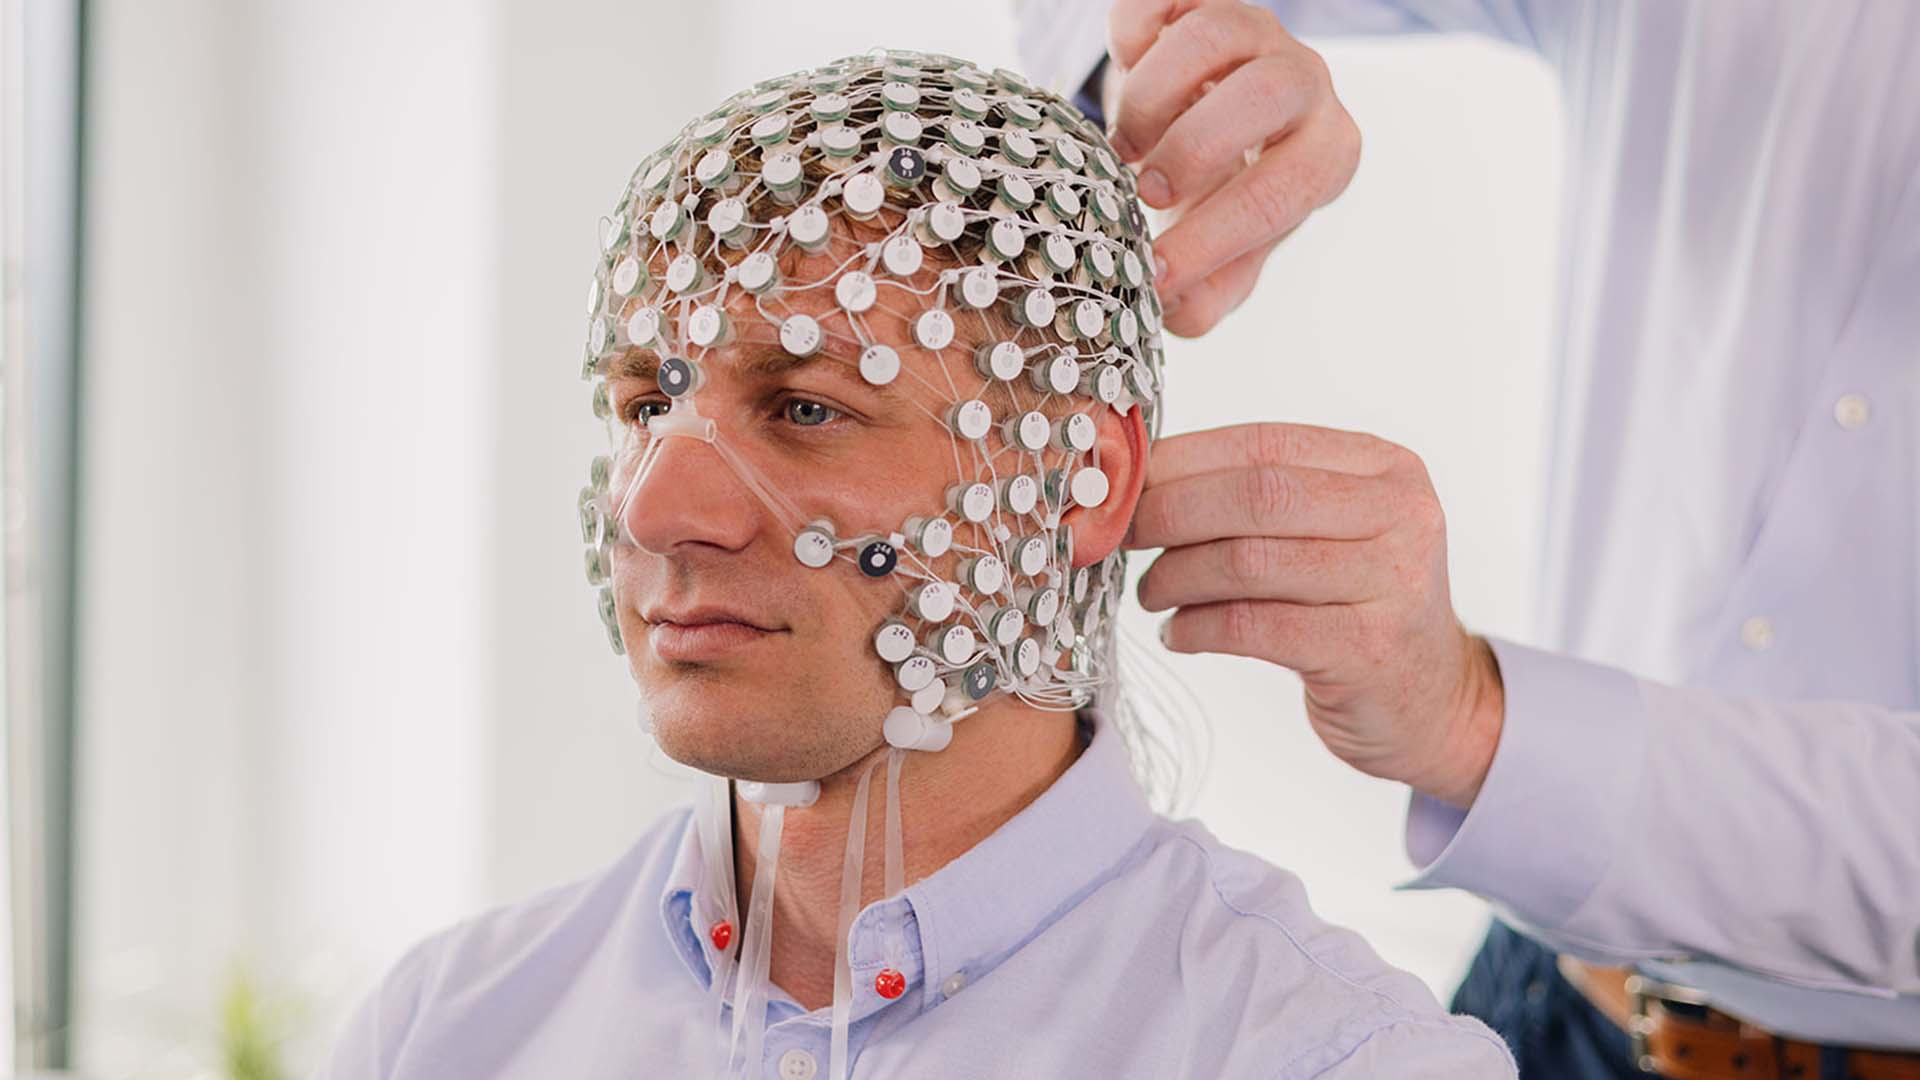
\includegraphics[width=\linewidth,height=20mm,keepaspectratio]{assets/history/egi-hd-eeg-sensor-net.jpg}
      \par{\tiny HD-EEG Geodesic Sensor Net\par}\smallskip
      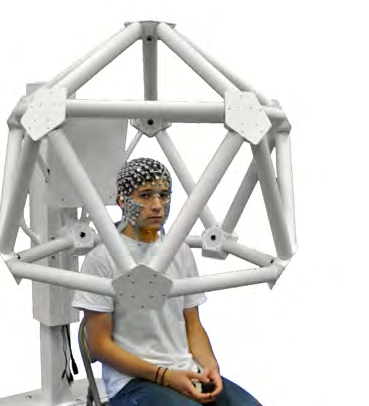
\includegraphics[width=\linewidth,height=20mm,keepaspectratio]{assets/history/egi-geodesic-camera-dome.png}
      \par{\tiny Geodesic Photogrammetry System\par}
  \end{columns}
  \smallskip{\tiny\color{NTXMuted}Equipment illustrations: \href{https://www.magstim.com/ges-500/}{Magstim EGI}; \href{https://www.egi.com/research-division/electrical-source-imaging/photogrammetry-sensor-digitization}{EGI sensor-digitization brochure}\par}
  
  
  \note{[00:30--01:15] Briefly connect my dual background in biochemistry/molecular biology and experimental psychology with building equipment in a student research lab. I then worked with Karl Pribram on HD-EEG, and at Electrical Geodesics under Don Tucker, becoming software engineering manager. Morgan reports successfully leading the product through FDA approval and CE marking. This is his firsthand career account; no product model, date, regulatory submission number or specific FDA pathway has been independently established. Do not infer PMA versus 510(k), sole responsibility, or clearance of all later products. The equipment images are later official illustrations, not the specific product or generation taken through regulation. This experience connects hands-on engineering to translating a product beyond a research lab.}
\end{frame}

% Selected from biography.tex
\begin{frame}{About Me}
  \begin{columns}[c,onlytextwidth]
    \column{.55\textwidth}
      \small
      \textbf{Biopunk Lab}\par
      Founding Member --- synthetic neurobiology\par\smallskip
      \textbf{Neurotech@Frontier Tower}\par
      Lead\par\smallskip
      \textbf{Other Minds Lab}\par
      Co-founder\par\smallskip
      \textbf{Orthogonal Research \& DevoWorm Group}\par
      Lab Member\par\smallskip
      \textbf{NeuroTechX}\par
      Executive Director
    \column{.41\textwidth}
      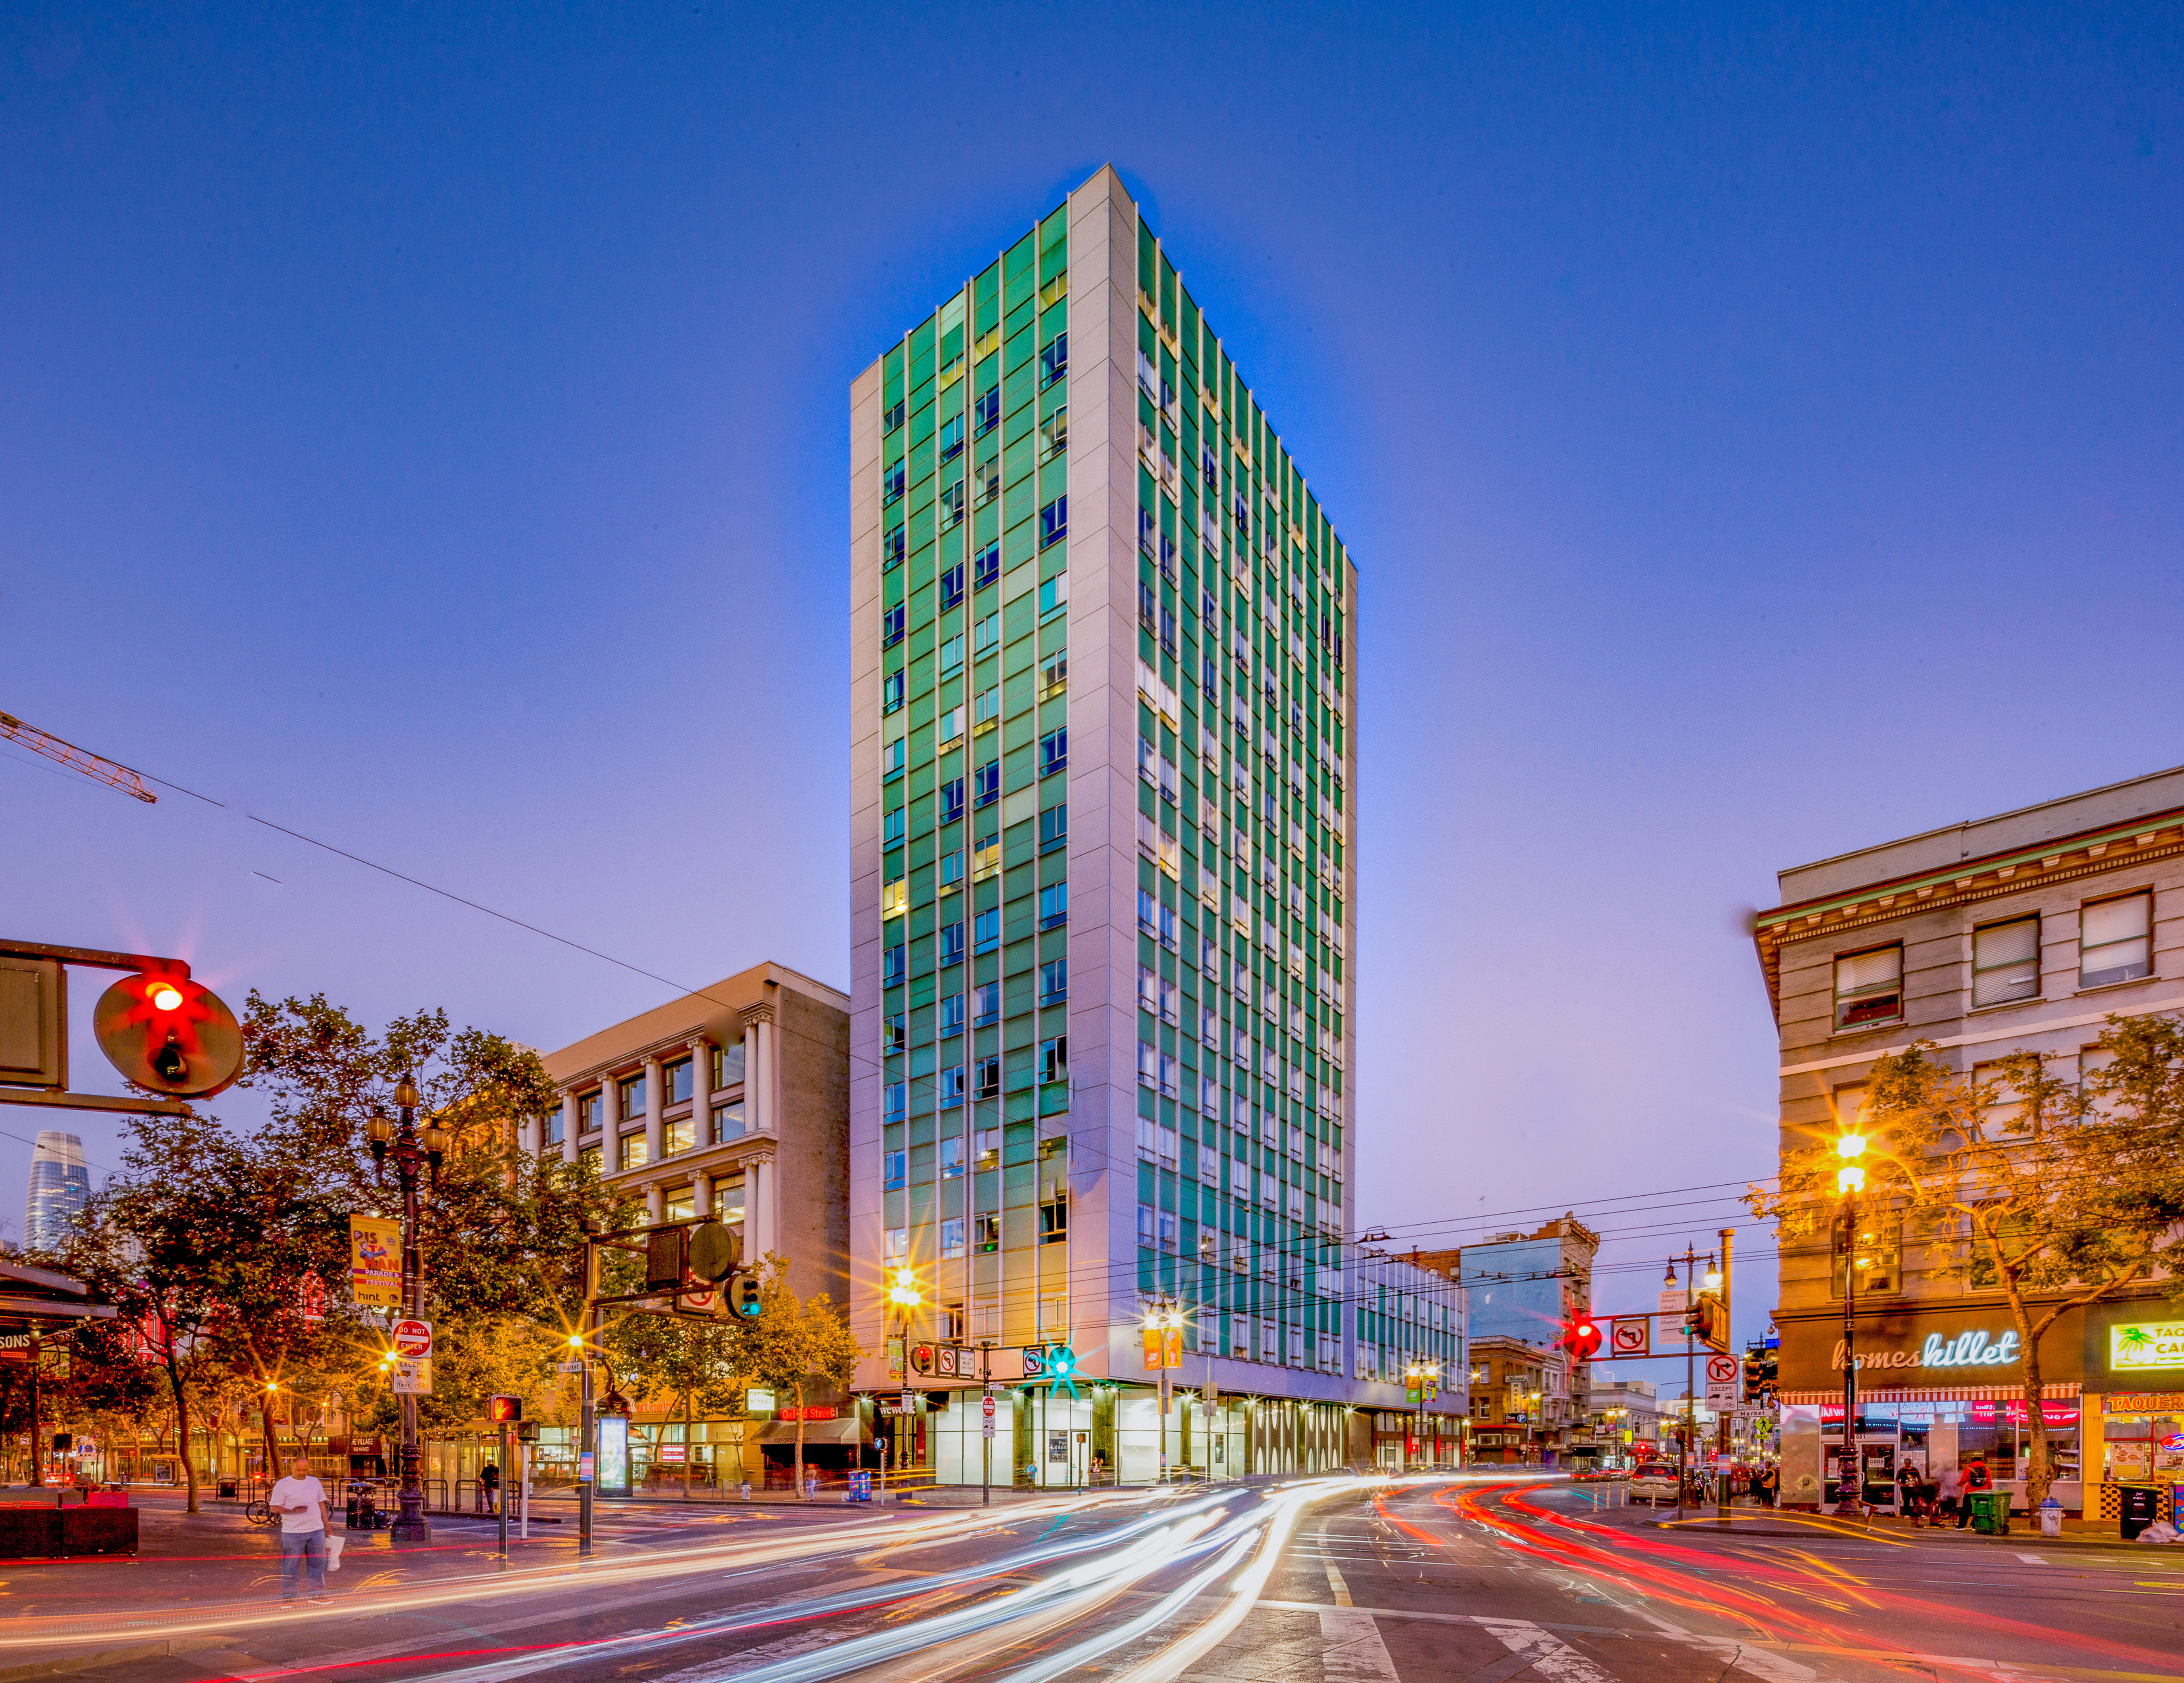
\includegraphics[width=\linewidth,height=52mm,keepaspectratio]{assets/history/frontier-tower-exterior.jpg}
      \par\smallskip
      {\tiny Frontier Tower, 995 Market Street\par
      Earlier exterior photo: \href{https://www.995market.com/}{Colliers / 995 Market listing}}
  \end{columns}
  
  \note{[01:15--01:45] Briefly introduce the current roles on screen. These are Morgan's own biographical details. The tower image is an earlier property-listing photograph. Move quickly from my background to what we build together.}
\end{frame}

\section{NeuroTechX}

% Selected from slides.tex
\begin{frame}{What is NeuroTechX?}
  \begin{columns}[T,onlytextwidth]
    \column{.52\textwidth}
      \NTXPoint{A nonprofit community}{Connecting neuroscience and technology.}
      \NTXPoint{Founded in Montr\'eal in 2015}{City chapters, student groups, and open projects.}
      \NTXPoint{Three pillars}{Community, education, and professional development.}
    \column{.43\textwidth}
      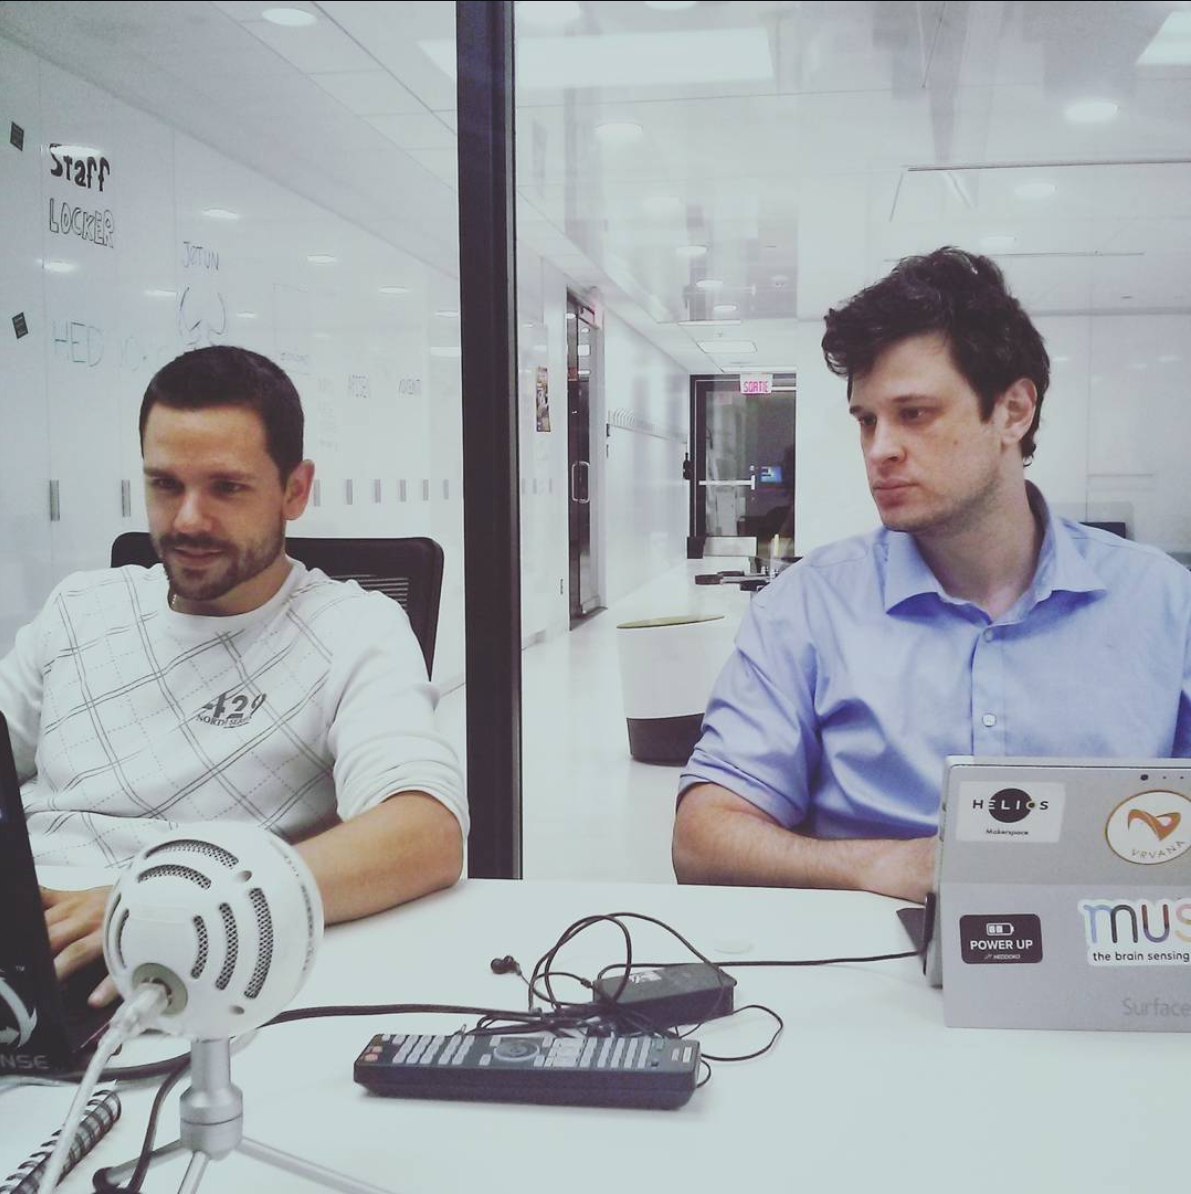
\includegraphics[width=\linewidth,height=47mm,keepaspectratio]{assets/people/neurotechx-instagram-1.png}
      \par\smallskip{\scriptsize Sydney Swaine-Simon and Yannick Roy\par}
  \end{columns}
  \NTXSource{https://www.neurotechx.org/about}{NeuroTechX: Our Story; photo from NeuroTechX's Instagram archive}
  
  \note{[01:45--02:45] Introduce the nonprofit and the three pillars. The point is to connect people across disciplines, not just to distribute devices. Avoid membership totals: this slide does not establish how many people or chapters are active today.}
\end{frame}

% Selected from slides.tex
\begin{frame}{What do we do?}
  \begin{columns}[c,onlytextwidth]
    \column{.43\textwidth}
      \small
      \NTXPoint{Community building}{Chapter meetings, hacknights, student chapters, hackathons, and student competitions.}
      \NTXPoint{Make learning accessible}{The NeuroTech Primer, workshops, webinars, and open science.}
      \NTXPoint{Build and share tools}{EEG-ExPy, MOABB, and contributions across open neurotechnology.}
    \column{.53\textwidth}
      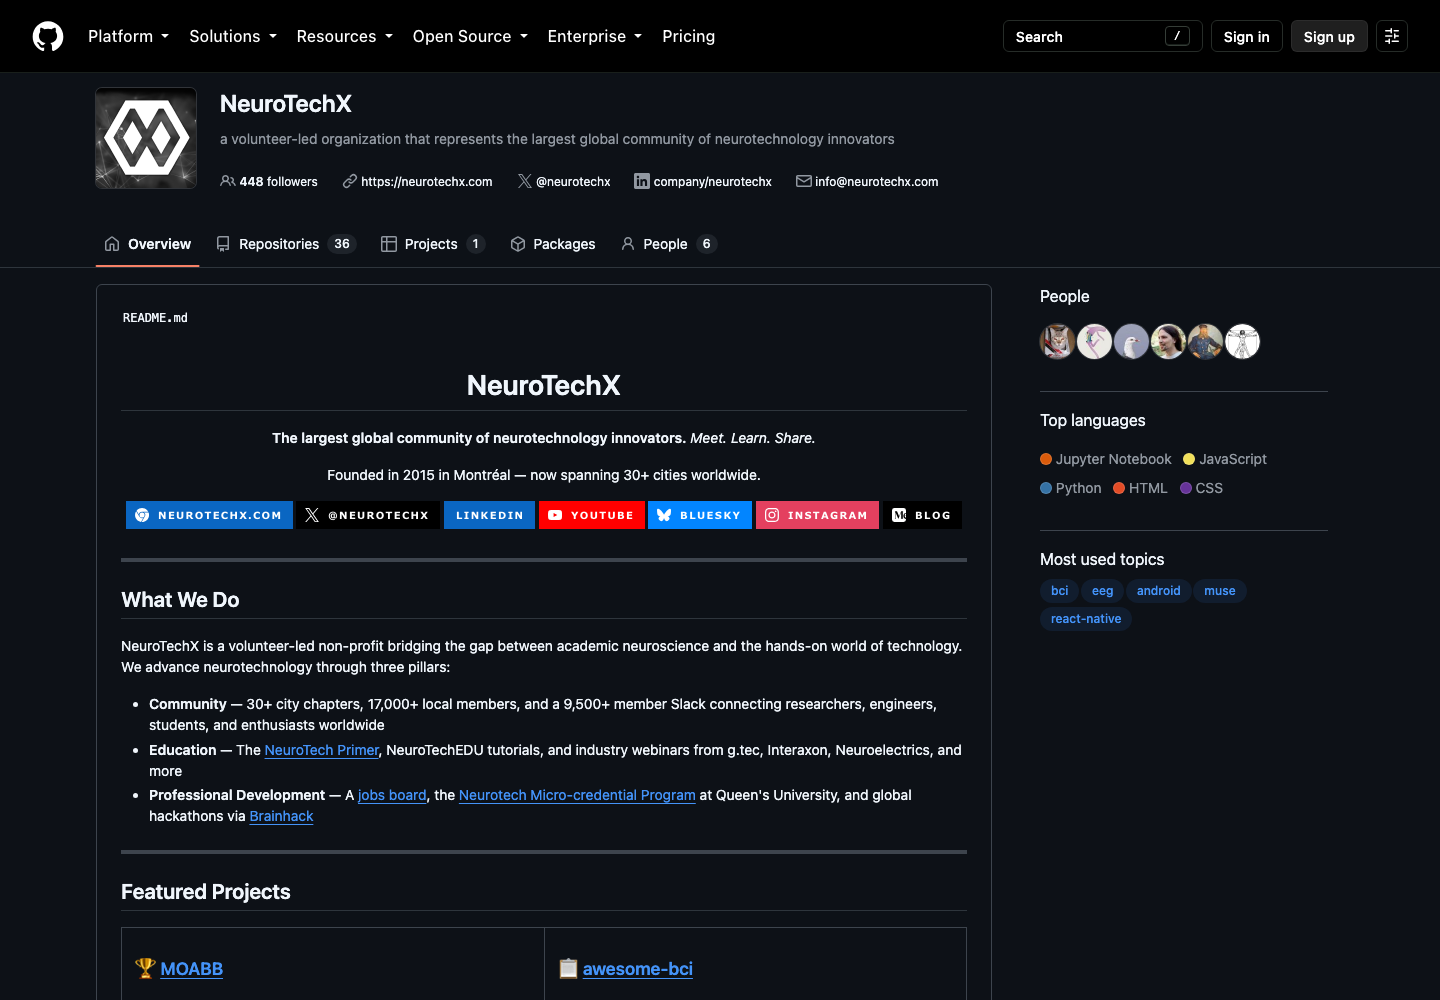
\includegraphics[width=\linewidth,height=49mm,keepaspectratio]{assets/history/neurotechx-github-org.png}
      \par\smallskip{\scriptsize \href{https://github.com/NeuroTechX}{github.com/NeuroTechX}\par}
  \end{columns}
  {\tiny\color{NTXMuted}Sources: \href{https://www.neurotechx.org/education}{NeuroTechX education}; GitHub organization homepage, captured September 6, 2026\par}
  
  \note{[02:45--03:45] Preview the participation routes: local gatherings, education and shared tools. Not everyone starts by writing code. Hardware builders, researchers, writers, organizers and students all have ways to contribute. The GitHub image is a dated snapshot, not an audited activity total.}
\end{frame}

\section{Community Building}
\NTXDivider{Community Building}

% Selected from first-wave-bci.tex
\begin{frame}{The first wave of BCI: control your world}
  \begin{columns}[c,onlytextwidth]
    \column{.61\textwidth}
      \small
      \NTXPoint{Consumer headsets opened the door}{Games, feedback, and device-control experiments made brain signals something people could explore outside a lab.}
      \NTXPoint{The promise brought people together}{Hardware to try, software to write, and results to compare: a starting point for hacknights and community building.}
      {\small\textbf{Early entry points}\par}
      {\small Muse \enspace EMOTIV \enspace NeuroSky \enspace OpenBCI\par}
      \medskip
      {\small\textbf{The ecosystem kept growing}\par}
      {\small Neurosity \enspace BrainBit \enspace Bitbrain \enspace MindAffect\par}
    \column{.35\textwidth}
      \centering
      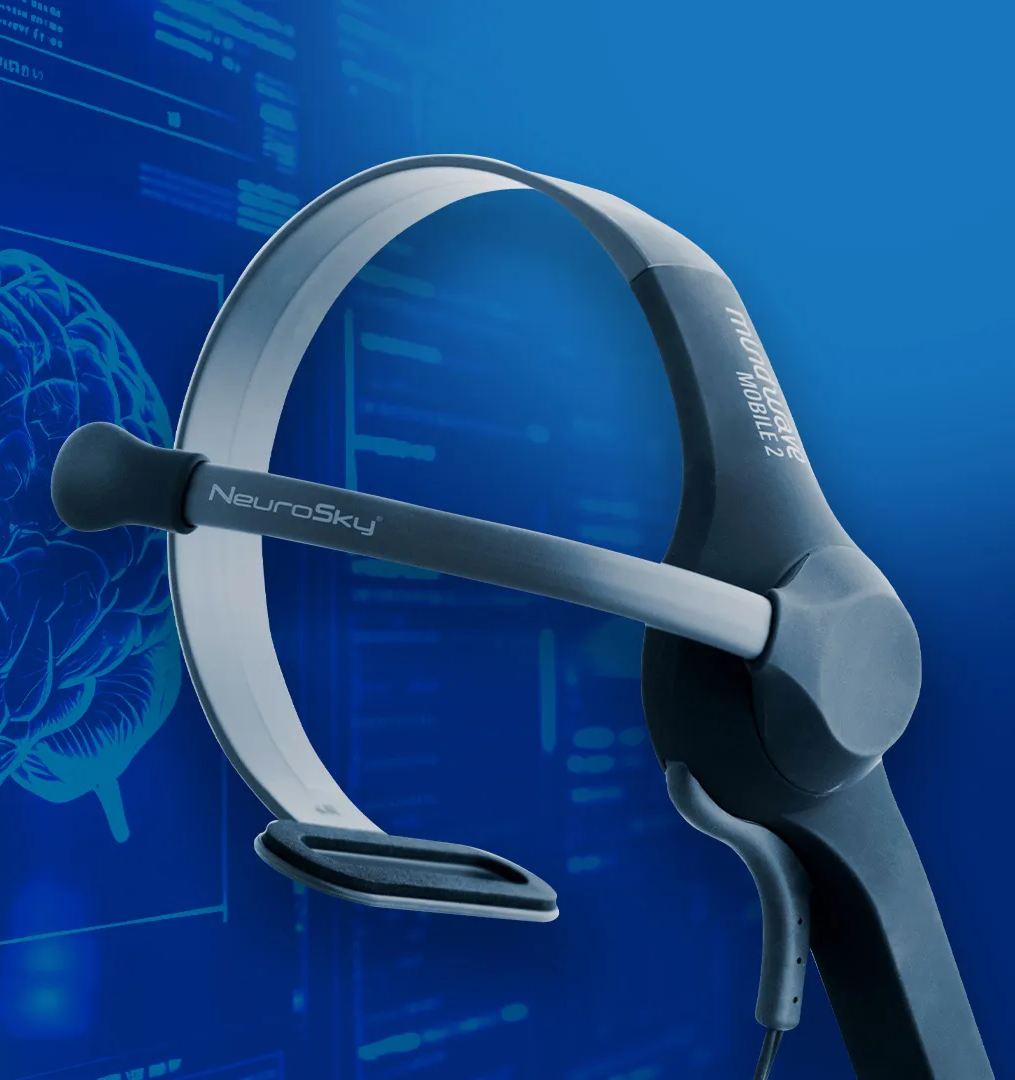
\includegraphics[width=\linewidth,height=40mm,keepaspectratio]{assets/history/neurosky-mindwave-mobile2.png}\par\smallskip
      {\tiny NeuroSky MindWave Mobile 2\newline Later model illustrating the headset lineage\newline Photo: NeuroSky\par}
  \end{columns}
  {\tiny\color{NTXMuted}Morgan's community-history framing. Sources: \href{https://www.emotiv.com/blog/how-emotiv-epoc-changed-the-world-of-neurotechnology}{EMOTIV}; \href{https://choosemuse.com/pages/team}{Muse}; \href{https://neurosky.com/neurosky-products/mindwave-headset/}{NeuroSky}; \href{https://openbci.com/community/openbci-on-kickstarter/}{OpenBCI}\par}
  
  \note{[03:45--05:00] Use Morgan's first-wave framing: consumer and accessible headsets gave people something tangible to explore together. The promise attracted curiosity; learning to understand and use signals created shared work. The listed products arrived at different times and served different purposes. This is not the invention of BCI or a claim of unrestricted thought reading.}
\end{frame}

% Selected from slides.tex
\begin{frame}{A community across the world}
  \centering
  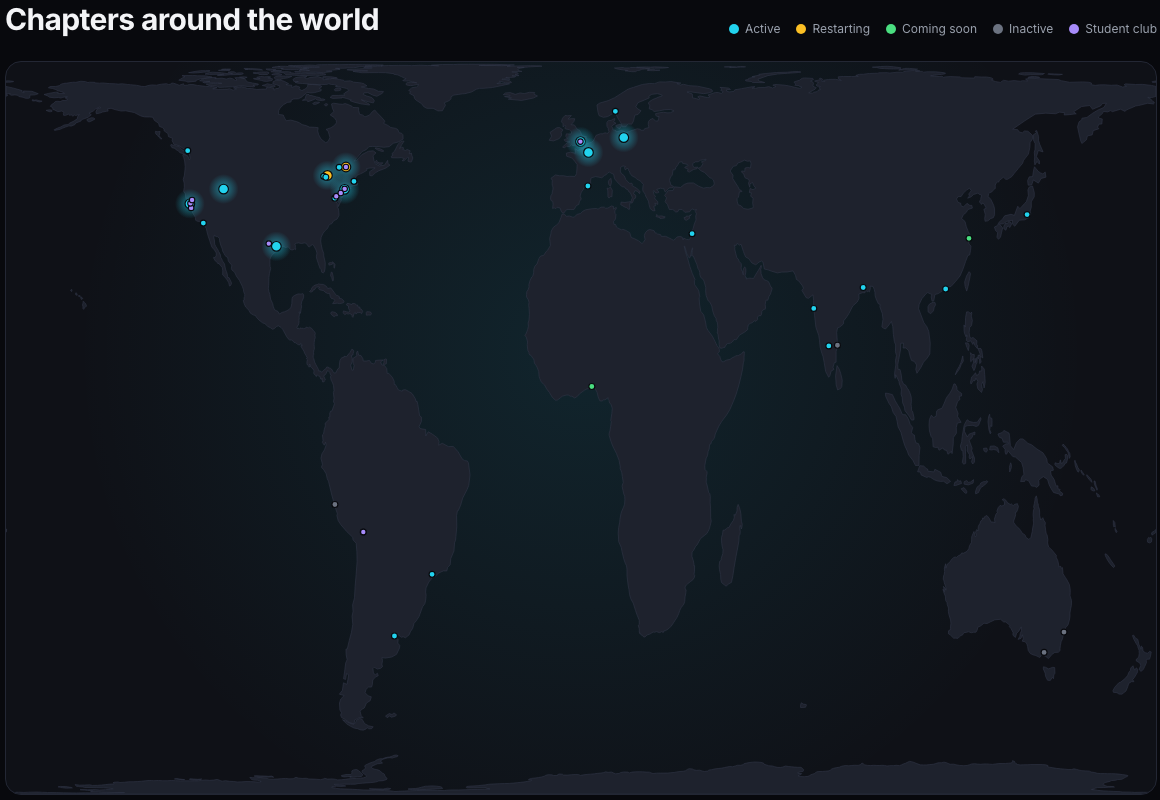
\includegraphics[width=\linewidth,height=55mm,keepaspectratio]{assets/chapters/neurotechx-community-map.png}
  \par\smallskip
  {\tiny\color{NTXMuted}\href{https://www.neurotechx.org/community}{NeuroTechX Community \& Chapters} --- website snapshot, September 6, 2026\par}
  
  \note{[05:00--05:30] Orient the audience, then move on. This is the September 6 website map, including multiple chapter statuses and student listings; it is not a census of active chapters. The lesson is that the network connects locally organized communities.}
\end{frame}

% Selected from slides.tex
\begin{frame}{Dans le vent}
  \framesubtitle{Local communities before NeuroTechX}
  \begin{columns}[T,onlytextwidth]
    \column{.47\textwidth}
      \textbf{San Francisco}\par\smallskip
      {\small Cognitive Technology Group\par}
      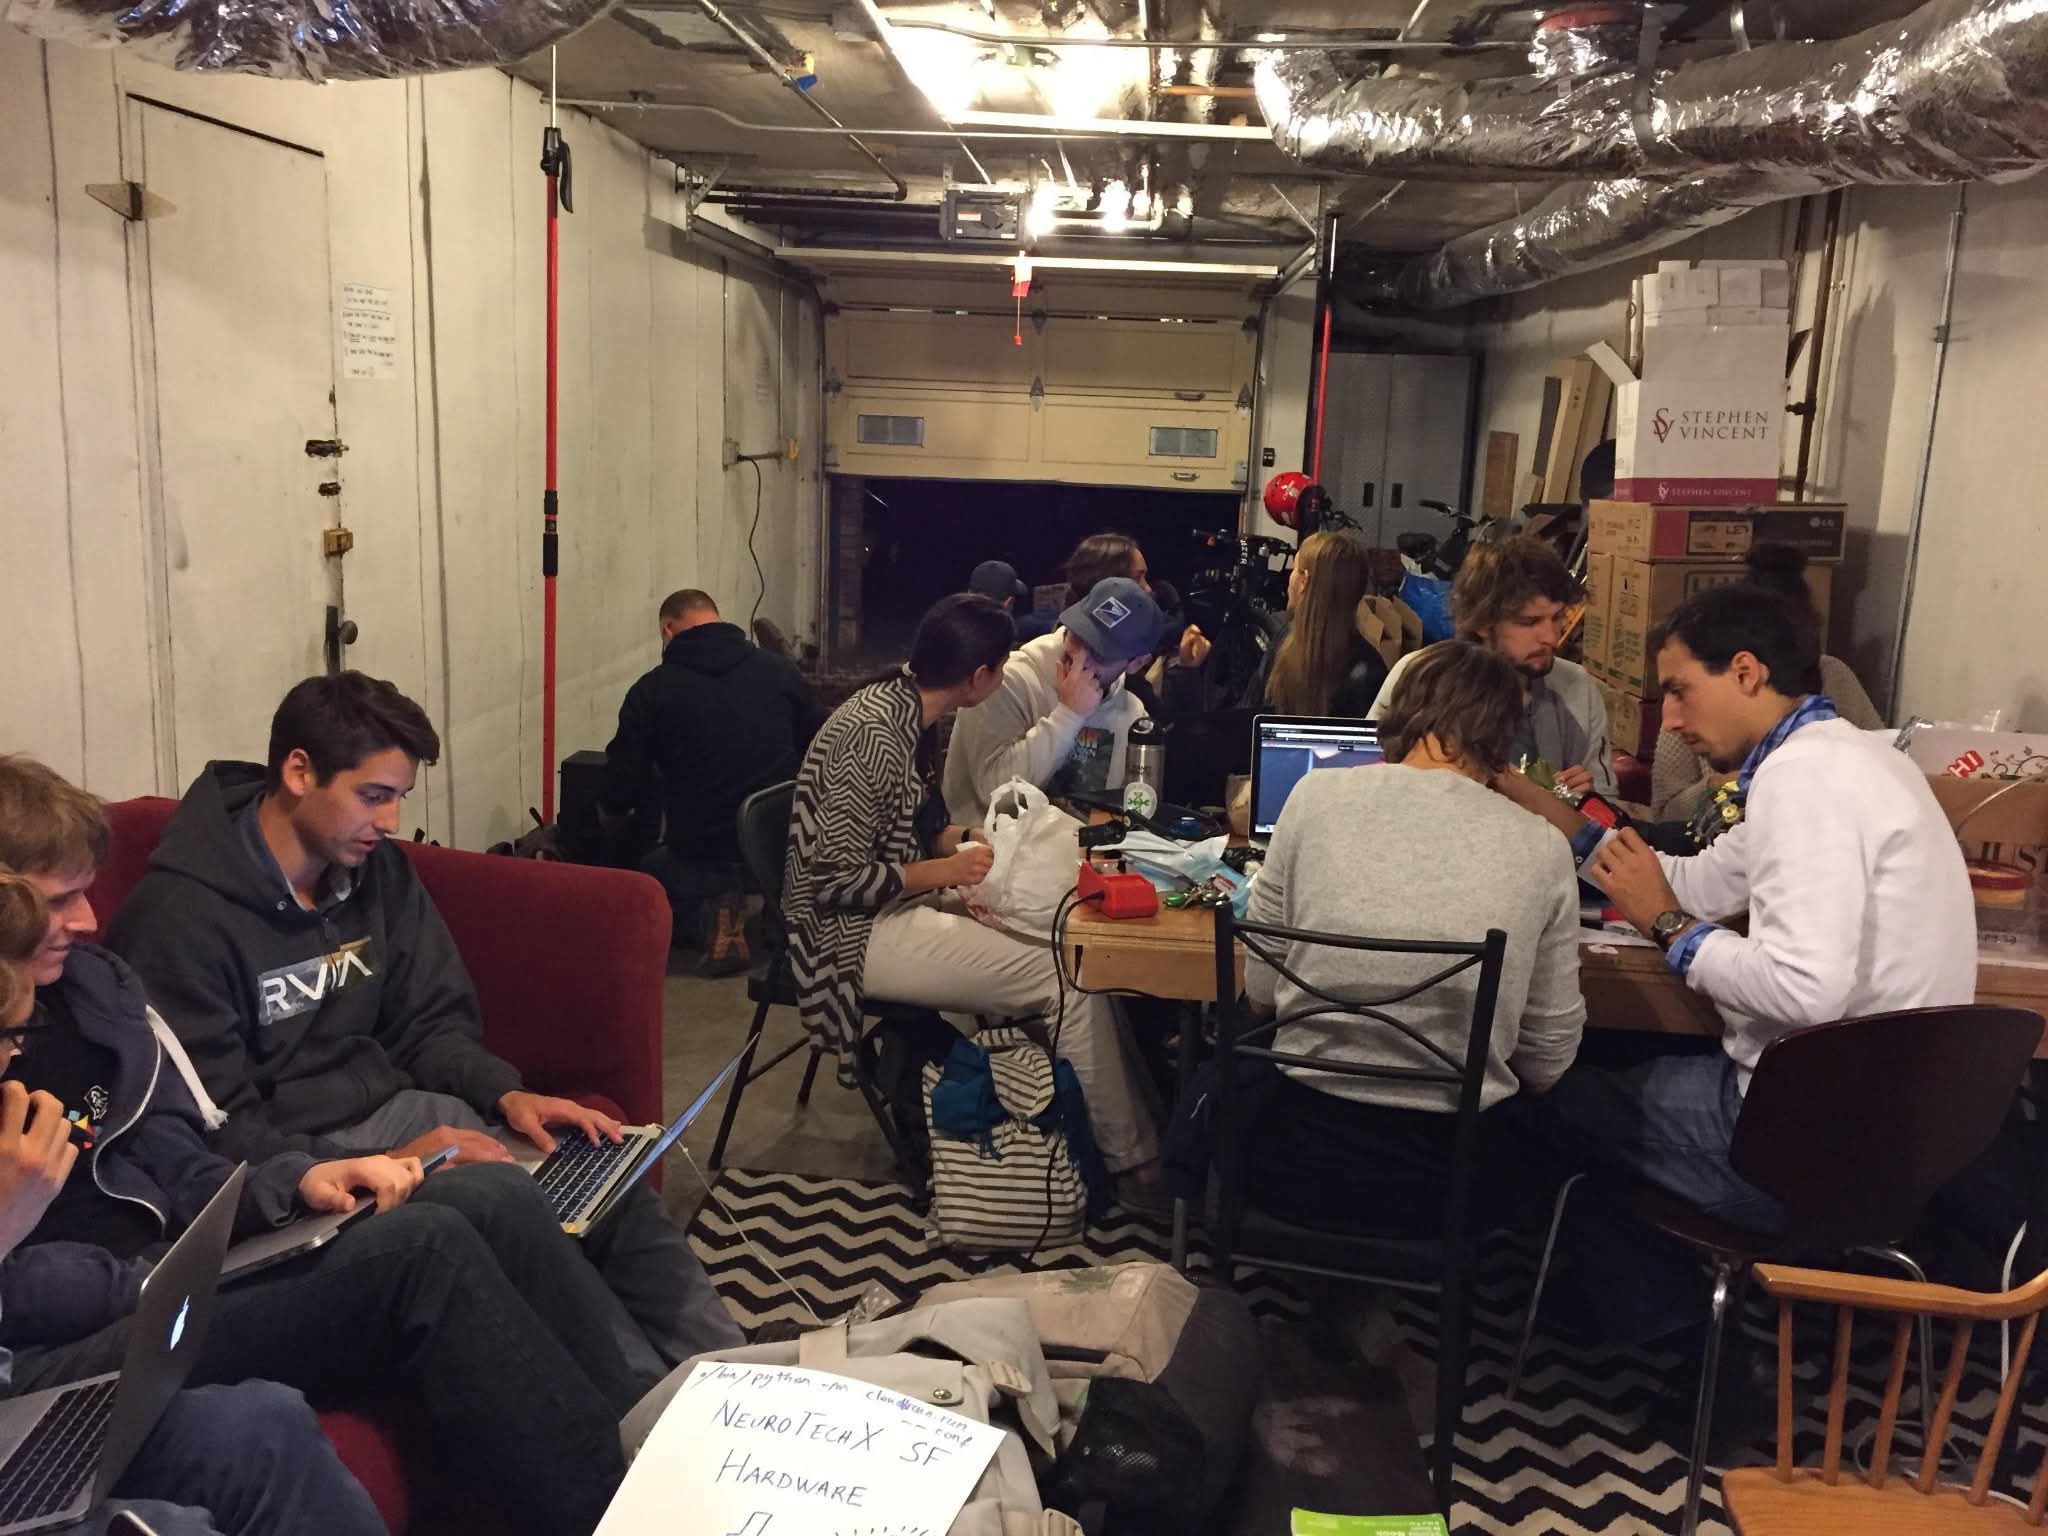
\includegraphics[width=\linewidth,height=28mm,keepaspectratio]{assets/chapters/san-francisco-original-hacknight.jpg}\par\smallskip
      {\small An existing community that became part of NeuroTechX\par}
      {\tiny Original SF Hacknights --- photo supplied by Morgan\par}
    \column{.47\textwidth}
      \textbf{Paris}\par\smallskip
      {\small CogLab --- September 2013\par}
      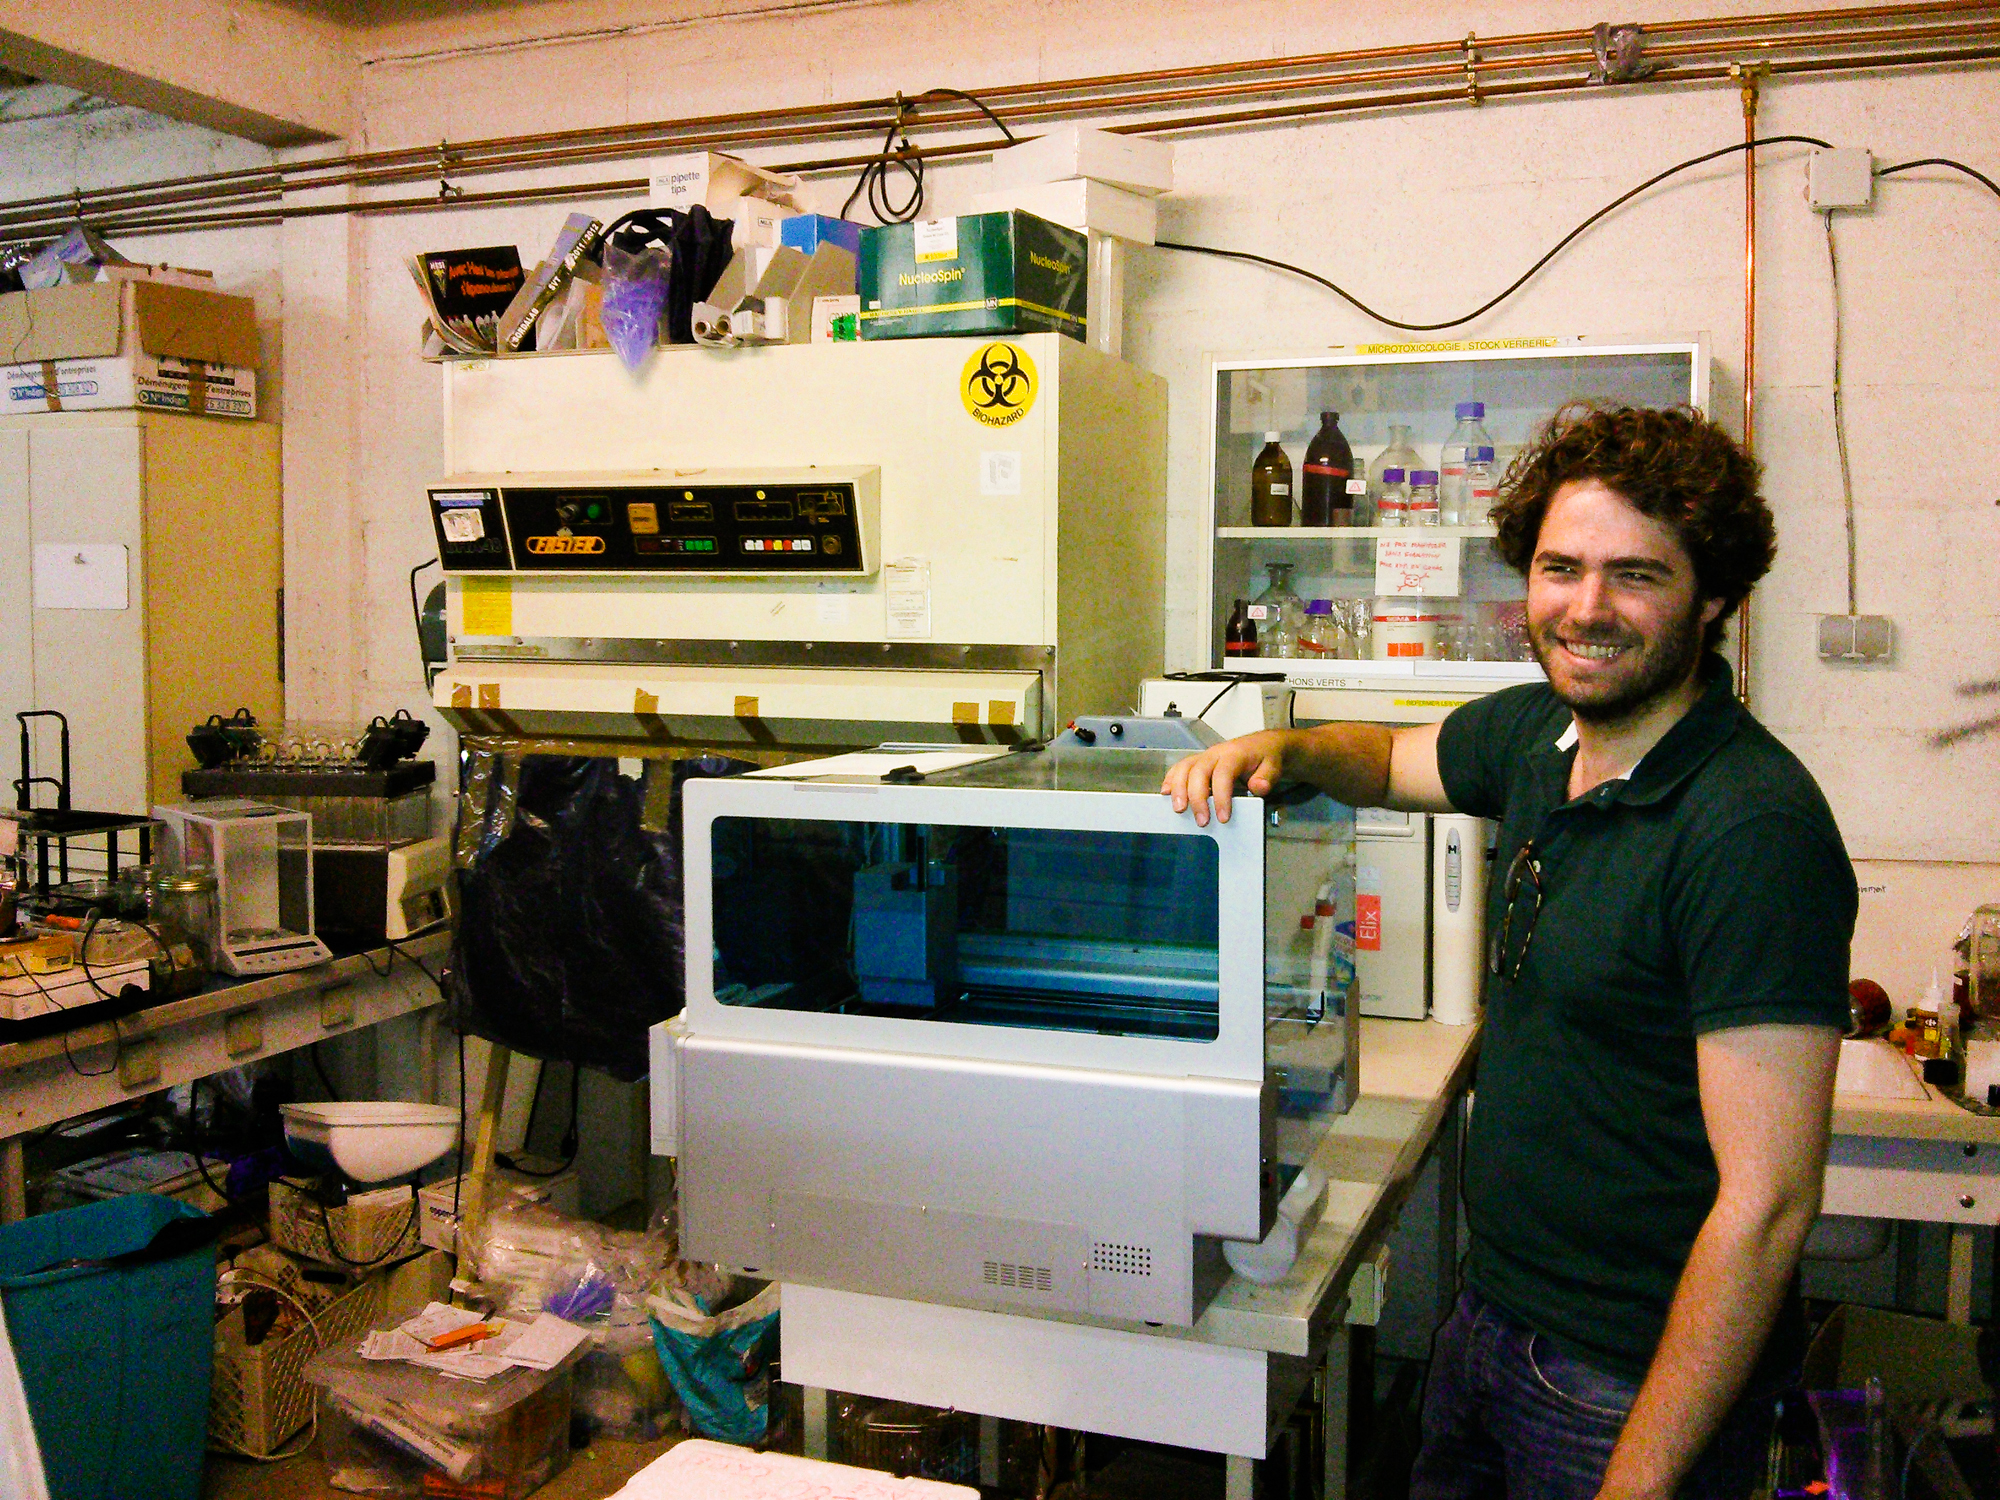
\includegraphics[width=\linewidth,height=28mm,keepaspectratio]{assets/chapters/la-paillasse-mitch-altman-2013.jpg}\par\smallskip
      {\small Launched by Romain Rouyer; incubated at La Paillasse\par}
      {\tiny La Paillasse, July 2013 --- \href{https://www.flickr.com/photos/maltman23/9379676390/}{Mitch Altman}, \href{https://creativecommons.org/licenses/by-sa/2.0/}{CC BY-SA 2.0}\par}
  \end{columns}
  {\tiny\color{NTXMuted}Sources: \href{https://github.com/Cognitive-Technology-Group}{Cognitive Technology Group archive}; \href{https://coglab.fr/about/coglab/}{CogLab: Gen\`ese}; Morgan Hough\par}
  
  \note{[05:30--07:00] Use San Francisco and Paris as the two examples of chapter development. Cognitive Technology Group and CogLab already had local identities, projects and gathering places. Morgan identifies their relationship to NeuroTechX. CogLab's history dates its launch to September 2013; the La Paillasse photograph is July 2013, not a picture of a NeuroTechX meeting. The lesson: work with existing local communities and organizers rather than assuming every chapter starts from zero. Invite Japan's existing groups to see themselves as collaborators.}
\end{frame}

% Selected from slides.tex
\begin{frame}{NeuroTechX Hacknights}
  \begin{columns}[T,onlytextwidth]
    \column{.52\textwidth}
      \NTXPoint{A recurring place to meet}{Newcomers and people already working on projects.}
      \NTXPoint{Across chapters}{San Francisco, Paris, and other local communities.}
      \NTXPoint{Work together}{Hardware, open science, software, and help from peers.}
    \column{.43\textwidth}
      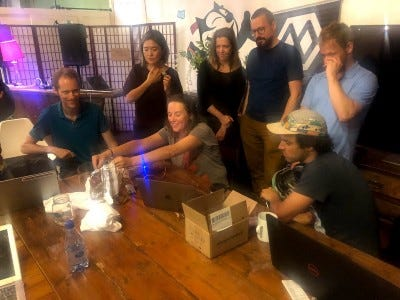
\includegraphics[width=\linewidth,height=47mm,keepaspectratio]{assets/chapters/sf-red-victorian-hacknight-2019.jpg}
      \par\smallskip{\scriptsize Hacknight at the Red Victorian, San Francisco\par}
  \end{columns}
  {\tiny\color{NTXMuted}Photo: Silicon Valley Global News / SVGN.io, published May 2019\par}
  
  \note{[07:00--08:30] Describe the recurring format: a newcomer brings curiosity or a question, meets people, and can return to work on something. Peer help and continuity matter more than a single impressive event. Morgan still cohosts Paris Hacknights. The new photo shows a NeuroTechX Hacknight at the Red Victorian in San Francisco, identified in the SVGN.io article published May 15, 2019. The exact photographed event date is not specified; do not label it as the forthcoming May 16 event or as Paris/CRI. This is not evidence of a guaranteed chapter-launch process.}
\end{frame}

% Selected from slides.tex
\begin{frame}{Buzz-in-Review: a shared annual chapter event}
  \begin{columns}[c,onlytextwidth]
    \column{.45\textwidth}
      \small
      \NTXPoint{The year in neurotechnology}{News and research for the general public.}
      \NTXPoint{Shared content, local conversations}{A common review for chapters to present and discuss.}
      \NTXPoint{A global format}{2021: 19 chapters across 10 online events.}
    \column{.51\textwidth}
      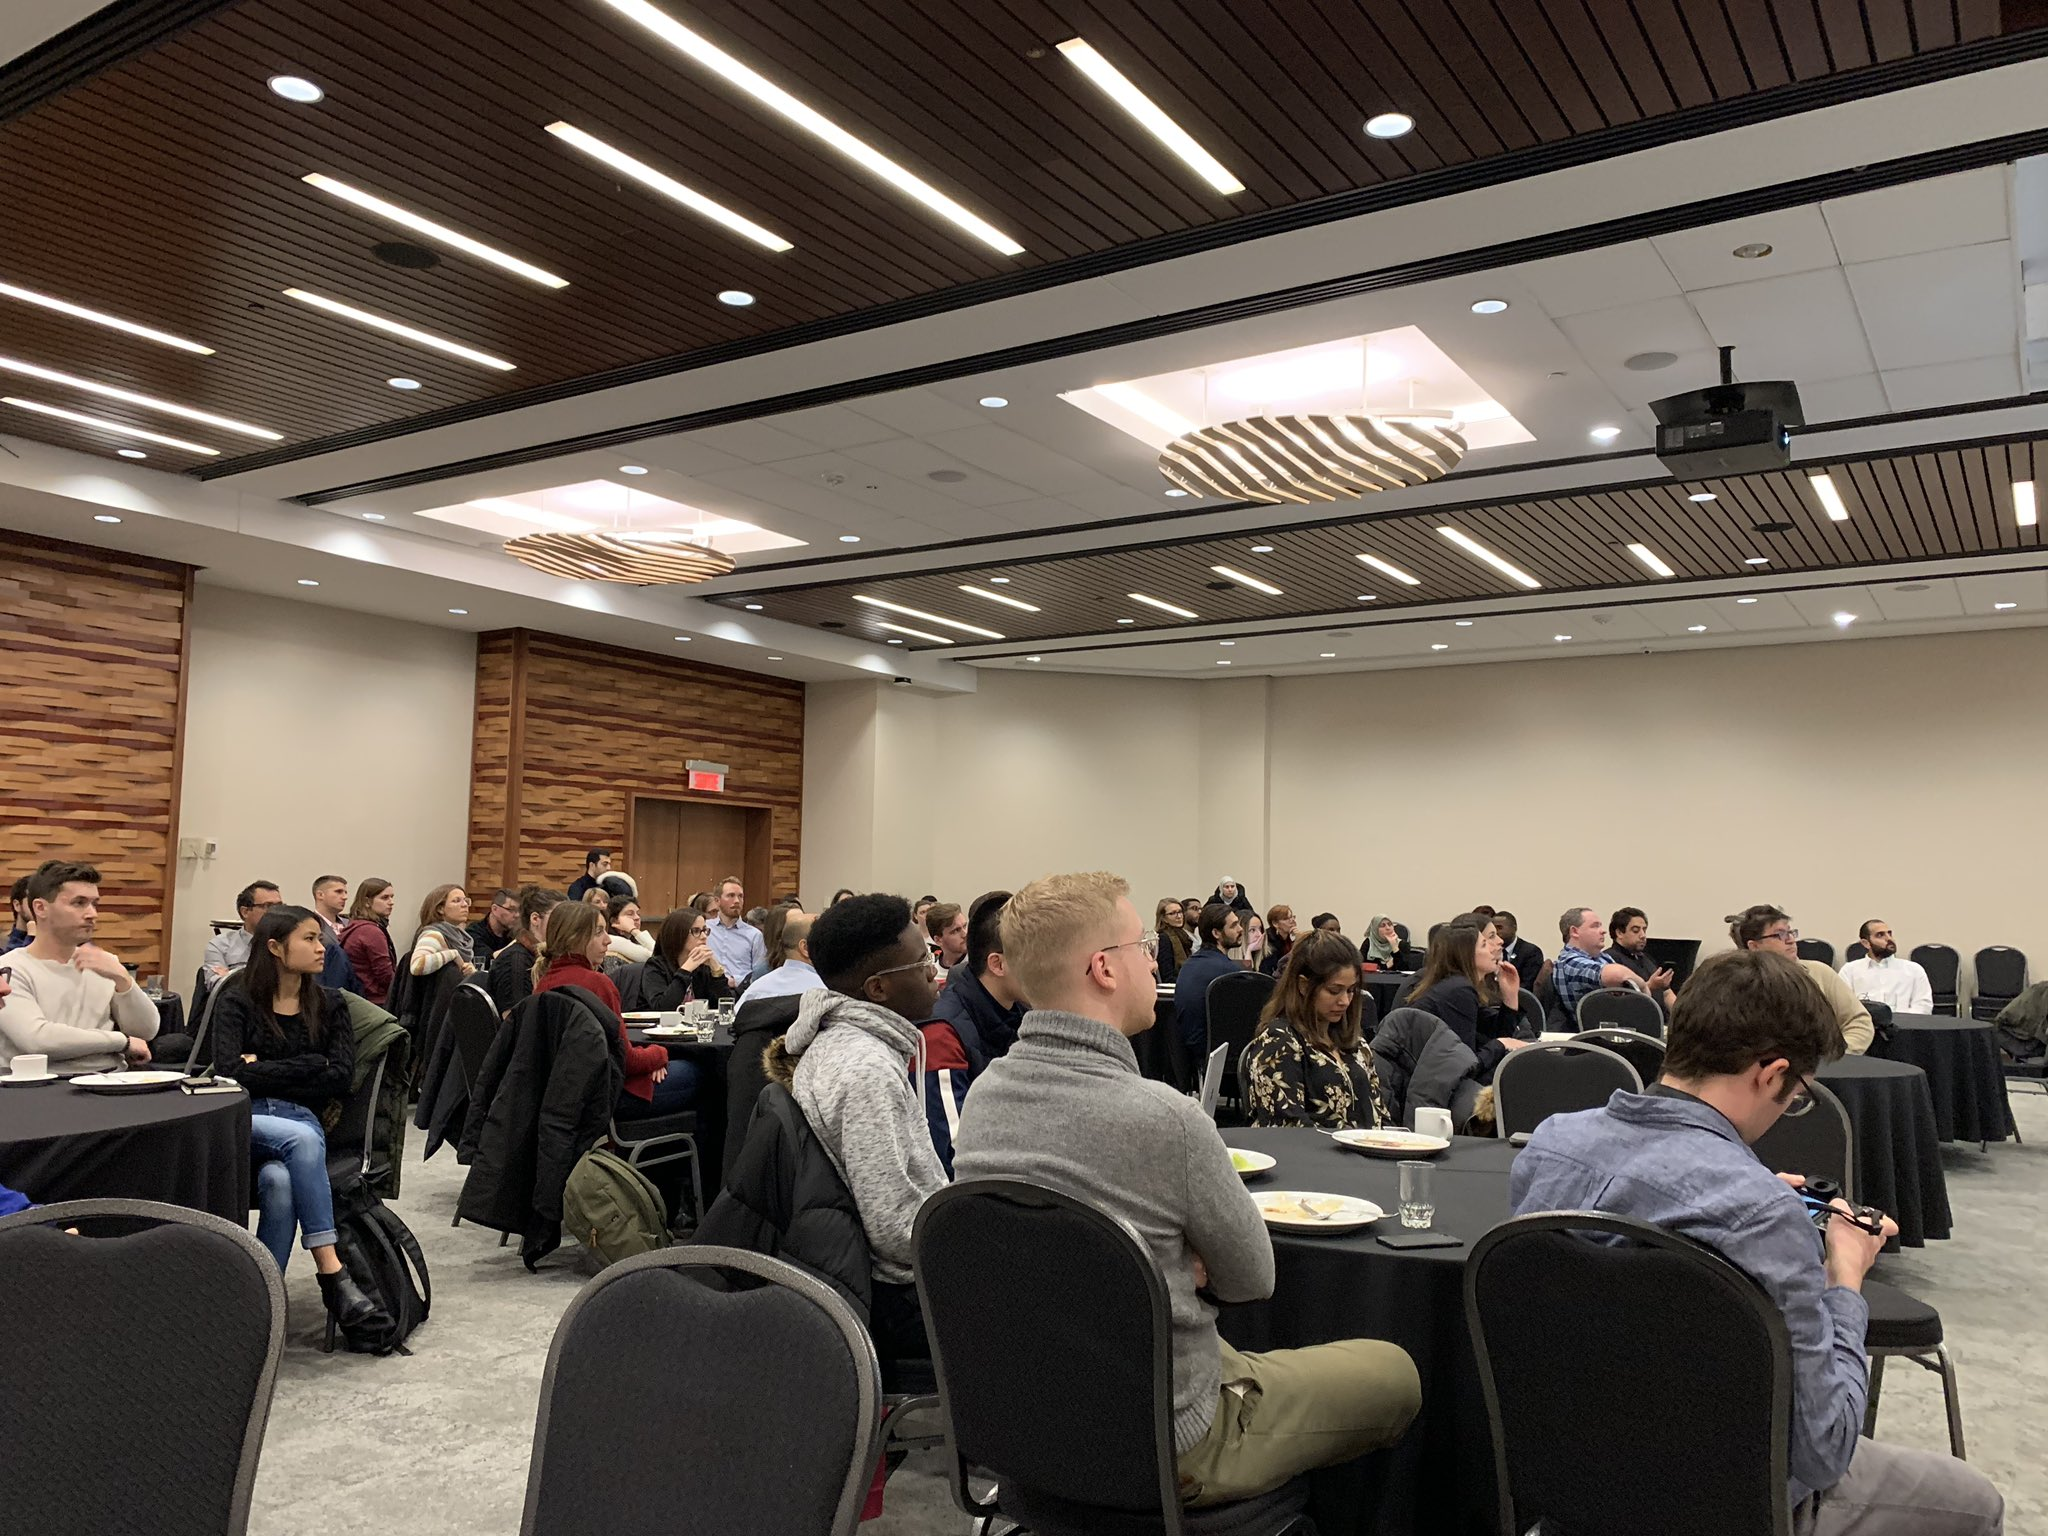
\includegraphics[width=\linewidth,height=45mm,keepaspectratio]{assets/chapters/montreal-buzz-in-review-2020.jpg}
      \par\smallskip{\scriptsize In person in Montr\'eal --- January 2020\par}
  \end{columns}
  {\tiny\color{NTXMuted}Sources: \href{https://neurotechx.com/ntxbir2021/}{Buzz in Review 2021}; photo: \href{https://twitter.com/NeuroTechMTL/status/1215643104847503363}{NeuroTechMTL}; \href{https://www.mcgill.ca/hbhl/channels/event/neurotech-buzz-review-2020-303563}{McGill / HBHL event listing}\par}

  \note{[08:30--09:45] Show how the network helps local organizers: shared research and news material becomes a local public conversation. The 2021 program listed 19 chapters across 10 online events. The photo instead shows Montreal's January 2020 in-person event. Distinguish program listings from attendance. The lesson is reusable content with room for local discussion.}
\end{frame}

% Selected from slides.tex
\begin{frame}{NeuroTechX Content Laboratory}
  \begin{columns}[c,onlytextwidth]
    \column{.46\textwidth}
      \small
      \NTXPoint{Writers, editors, and designers}{Original articles and varied perspectives on neurotechnology.}
      \NTXPoint{Another way to contribute}{Explain the field, share a project story, or edit someone else's work.}
      \NTXPoint{A recent example}{The Future of Brain Medicine with Owen Muir\\Interview by Chay Carter, May 2026}
    \column{.50\textwidth}
      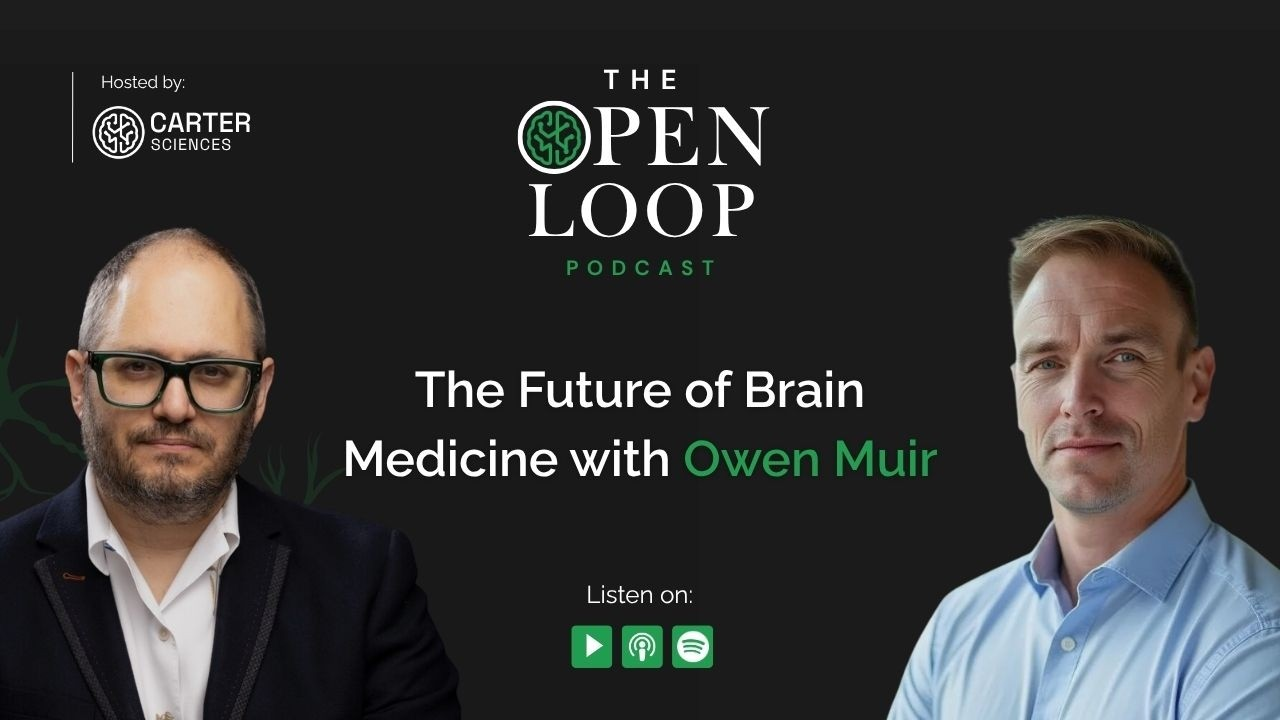
\includegraphics[width=\linewidth,height=40mm,keepaspectratio]{assets/history/content-lab-owen-interview.jpg}
      \par\smallskip{\scriptsize Original interview artwork: The Open Loop / Carter Sciences\par}
  \end{columns}
  {\tiny\color{NTXMuted}\href{https://medium.com/neurotechx/the-future-of-brain-medicine-with-owen-muir-a02360f770d5}{Read the Content Lab article}; \href{https://medium.com/neurotechx}{medium.com/neurotechx}; \href{https://www.youtube.com/watch?v=1ooyWf79Vyo}{original interview / image}\par}
  
  \note{[09:45--10:30] A route into community for writers, editors and designers. Explaining a project and sharing what was learned is a contribution. The image is original interview artwork for the Owen Muir example, not a Medium screenshot or an endorsement of clinical claims.}
\end{frame}

% Selected from slides.tex
\begin{frame}{The NeuroTechX newsletter: a long-running community resource}
  \begin{columns}[c,onlytextwidth]
    \column{.46\textwidth}
      \small
      \NTXPoint{An archive reaching back to 2015}{November 2015: NeuroTechX Digest \#1.}
      \NTXPoint{Keeping the community connected}{Research, industry developments, projects, events, and opportunities.}
      \NTXPoint{A record of the field as it develops}{\href{https://neurotechx.org/newsletter}{neurotechx.org/newsletter}}
    \column{.50\textwidth}
      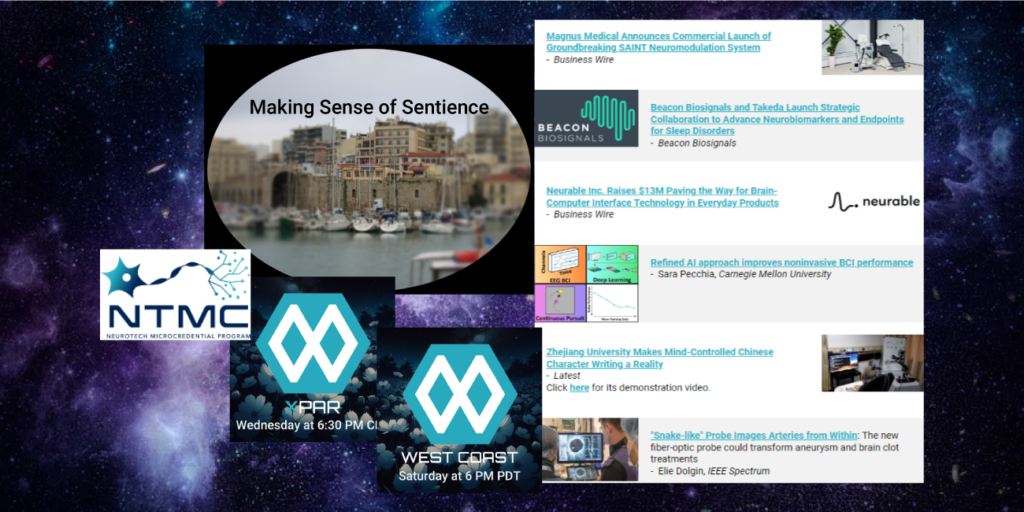
\includegraphics[width=\linewidth,height=40mm,keepaspectratio]{assets/history/ntx-newsletter-may2024.png}
      \par\smallskip{\scriptsize May 2024 newsletter --- official archive artwork\newline Image: NeuroTechX\par}
  \end{columns}
  \NTXSource{https://neurotechx.org/newsletter}{NeuroTechX newsletter archive; earliest listed edition: November 2015}

  \note{[10:30--11:00] The archive reaches back to November 2015. Emphasize continuity between events: people can keep following research, projects and opportunities. Do not claim uninterrupted publication or a field-wide longevity ranking. The artwork is from May 2024, not a current issue.}
\end{frame}

% Selected from slides.tex
\begin{frame}{Education: a way into the field}
  \begin{columns}[T,onlytextwidth]
    \column{.49\textwidth}
      \NTXPoint{The NeuroTech Primer}{An introduction to neurotechnology, including recording and stimulation.}
      \NTXPoint{Workshops and webinars}{Learn methods and hear from people working in the field.}
      \NTXPoint{Learning through contribution}{Developer meetings, open science, and shared projects.}
    \column{.46\textwidth}
      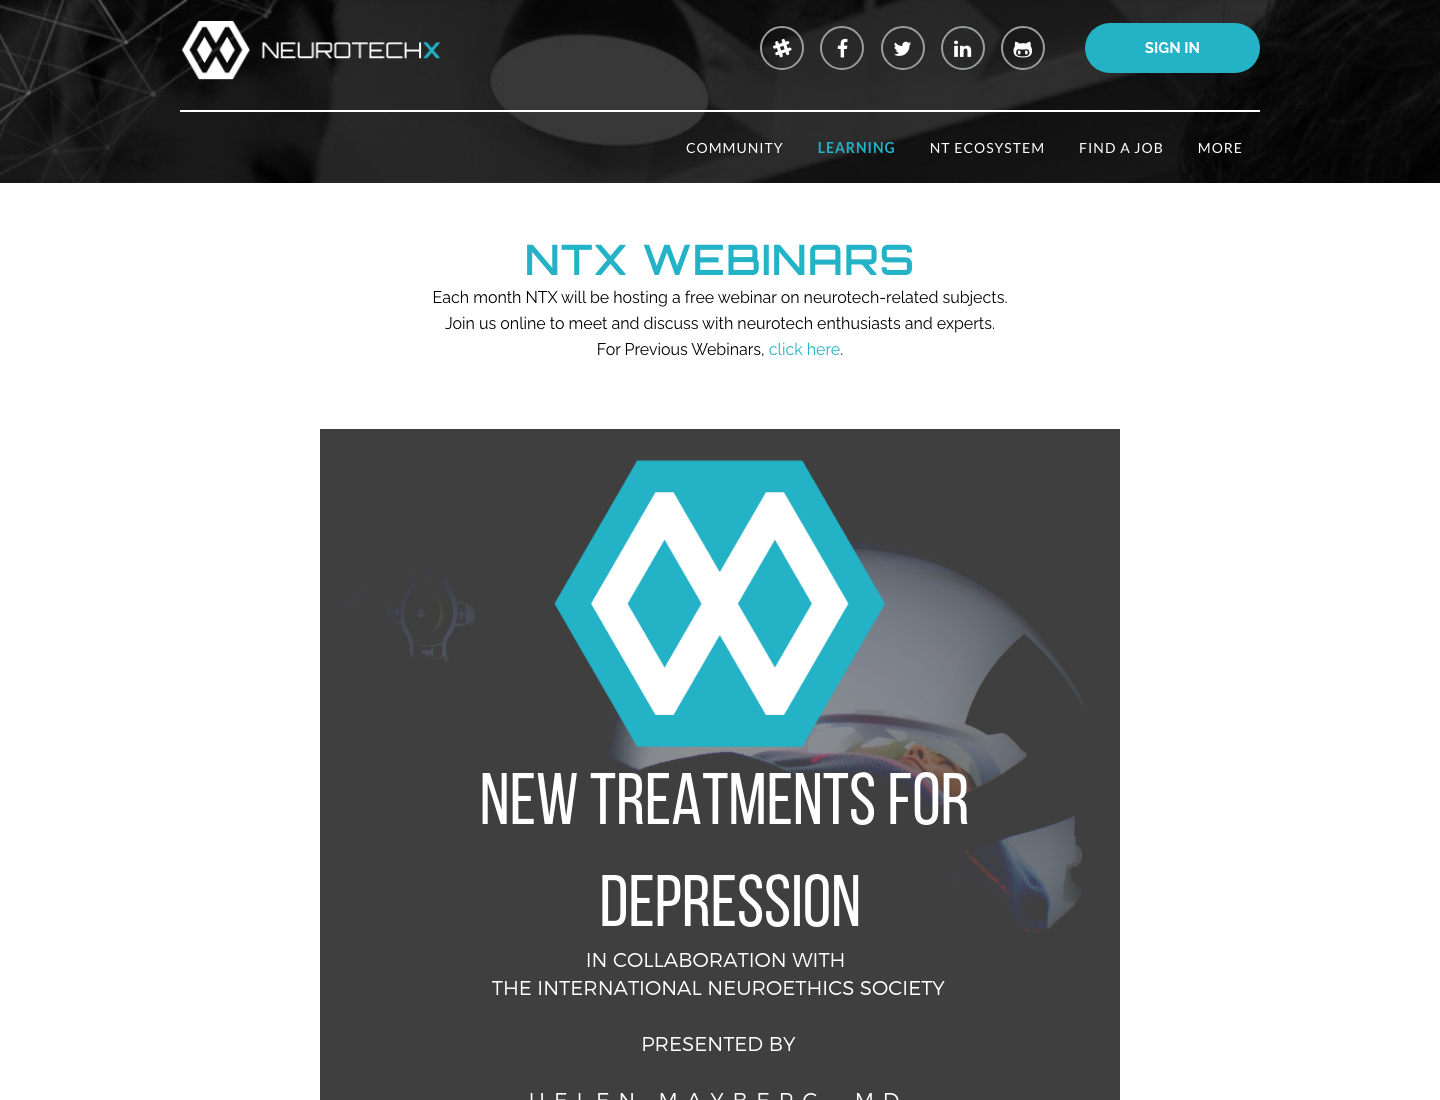
\includegraphics[width=\linewidth,height=46mm,keepaspectratio]{assets/history/neurotechx-webinar-page.png}
      \par\smallskip{\scriptsize \href{https://neurotechx.com/webinar/}{neurotechx.com/webinar}\par}
  \end{columns}
  \NTXSource{https://www.neurotechx.org/education}{NeuroTechX: The NeuroTech Primer, learning resources, and developer meetings}
  
  \note{[11:00--12:00] Connect the Primer, workshops and webinars to the next practical step: attend, ask a question, join a project, then help someone else. These are possible routes, not a mandatory funnel. The webinar screenshot illustrates the resource and is distinct from weekly pandemic Hacknights.}
\end{frame}

% Selected from slides.tex
\begin{frame}{EEG-ExPy: roots in muse-lsl and eeg-notebooks}
  \begin{columns}[T,onlytextwidth]
    \column{.66\textwidth}
      \NTXPoint{muse-lsl: access to the signal}{Alexandre Barachant's groundwork for streaming Muse EEG through Lab Streaming Layer.}
      \NTXPoint{eeg-notebooks: build the experiment}{Community-developed protocols combining recording, stimulus presentation, and analysis.}
      \NTXPoint{EEG-ExPy: carry the work forward}{John Griffiths and contributors; PsychoPy for experiments, MNE for analysis.}
    \column{.28\textwidth}
      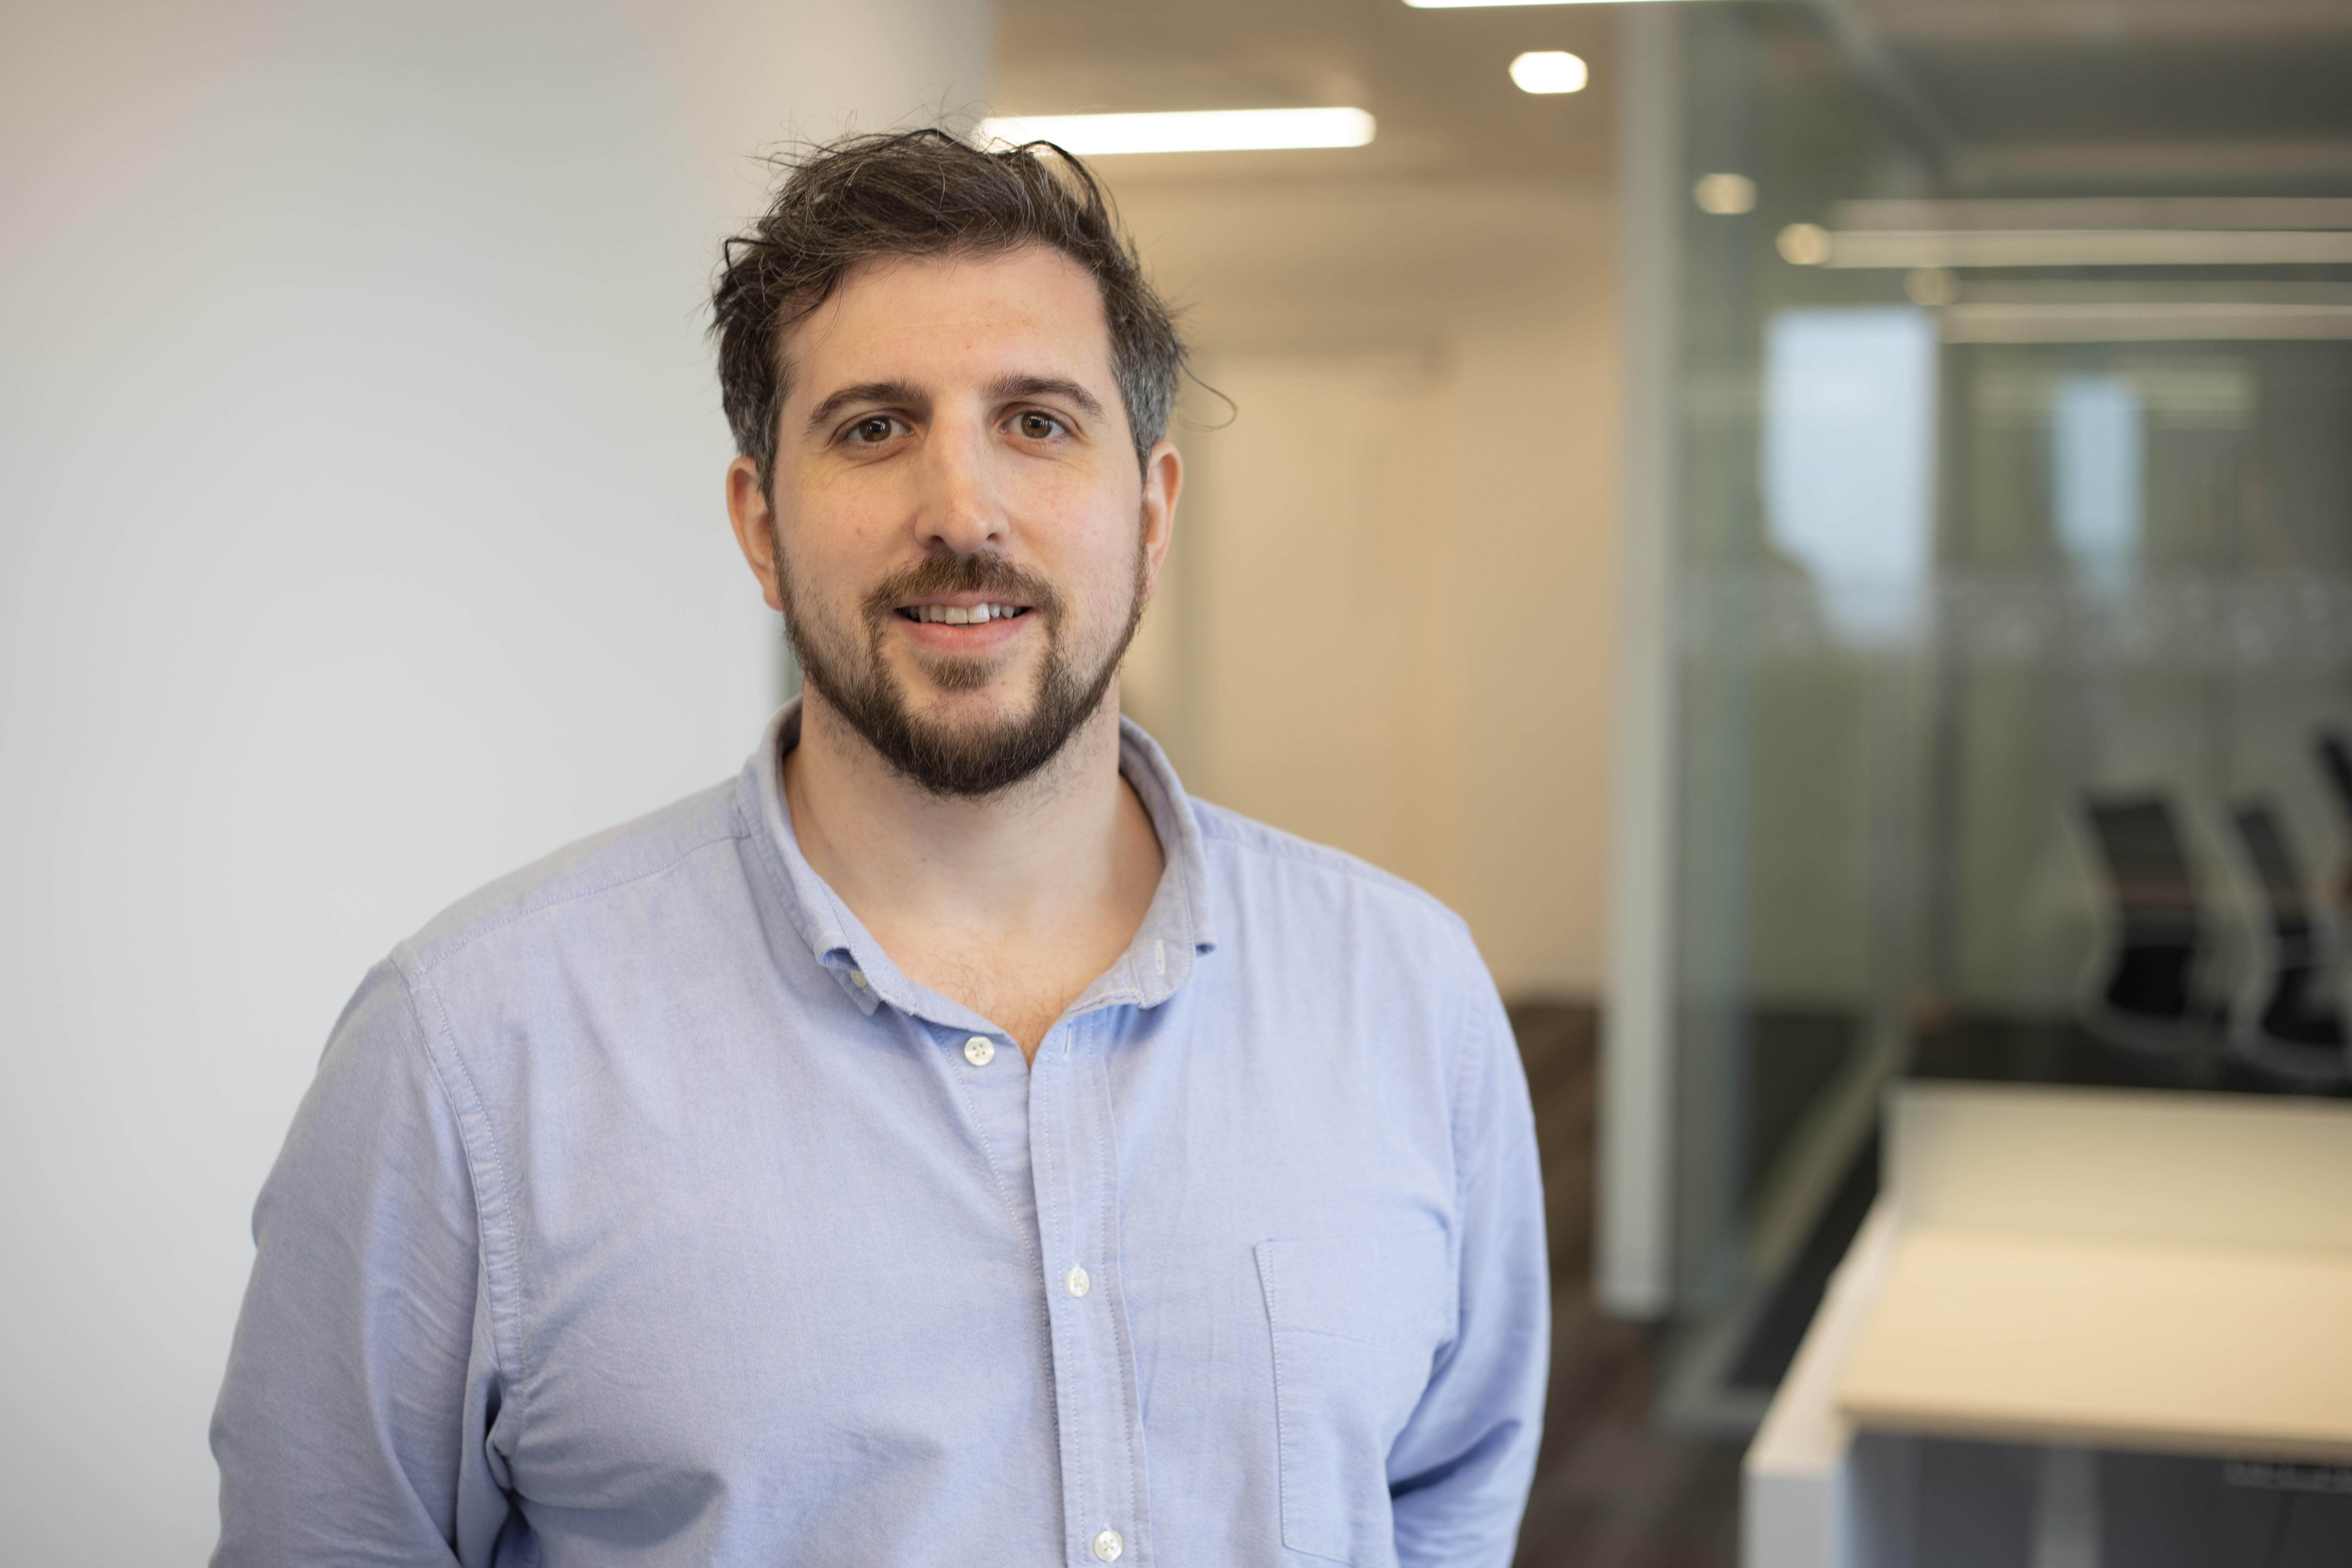
\includegraphics[width=\linewidth]{assets/people/john-griffiths.jpg}
      \par\smallskip{\small John Griffiths\par}
      \medskip{\scriptsize \href{https://www.crowdcast.io/e/brainhack-ontario/7}{Brainhack Ontario 2020\\introductory talk}\par}
  \end{columns}
  {\tiny\color{NTXMuted}Sources: \href{https://github.com/NeuroTechX/EEG-ExPy}{EEG-ExPy history and credits}; \href{https://www.grifflab.com/code_and_software/eeg-notebooks/}{Griffiths, 2019}; portrait: CAMH\par}
  \note{[12:00--13:00] A concrete path from accessible hardware to reproducible experiments. Credit Alexandre Barachant for muse-lsl and early groundwork, and John Griffiths and contributors for eeg-notebooks, later EEG-ExPy. muse-lsl is a foundational dependency, not an earlier name of the same project. Explain the connection between signal acquisition, experimental protocols and analysis. The community value is a starting point others can learn from and extend. The linked Brainhack Ontario talk was not independently viewed; do not describe its specific contents.}
\end{frame}

% Selected from dleeg.tex
\begin{frame}{MOABB: making BCI comparisons reproducible}
  \begin{columns}[c,onlytextwidth]
    \column{.43\textwidth}
      \small
      \NTXPoint{Mother of All BCI Benchmarks}{Open comparisons on public EEG datasets.}
      \NTXPoint{The 2024 benchmark study}{30 pipelines, 36 datasets:\newline motor imagery, P300, and SSVEP.}
      \NTXPoint{A shared research foundation}{Implementations and evaluations others can inspect and reproduce.}
    \column{.53\textwidth}
      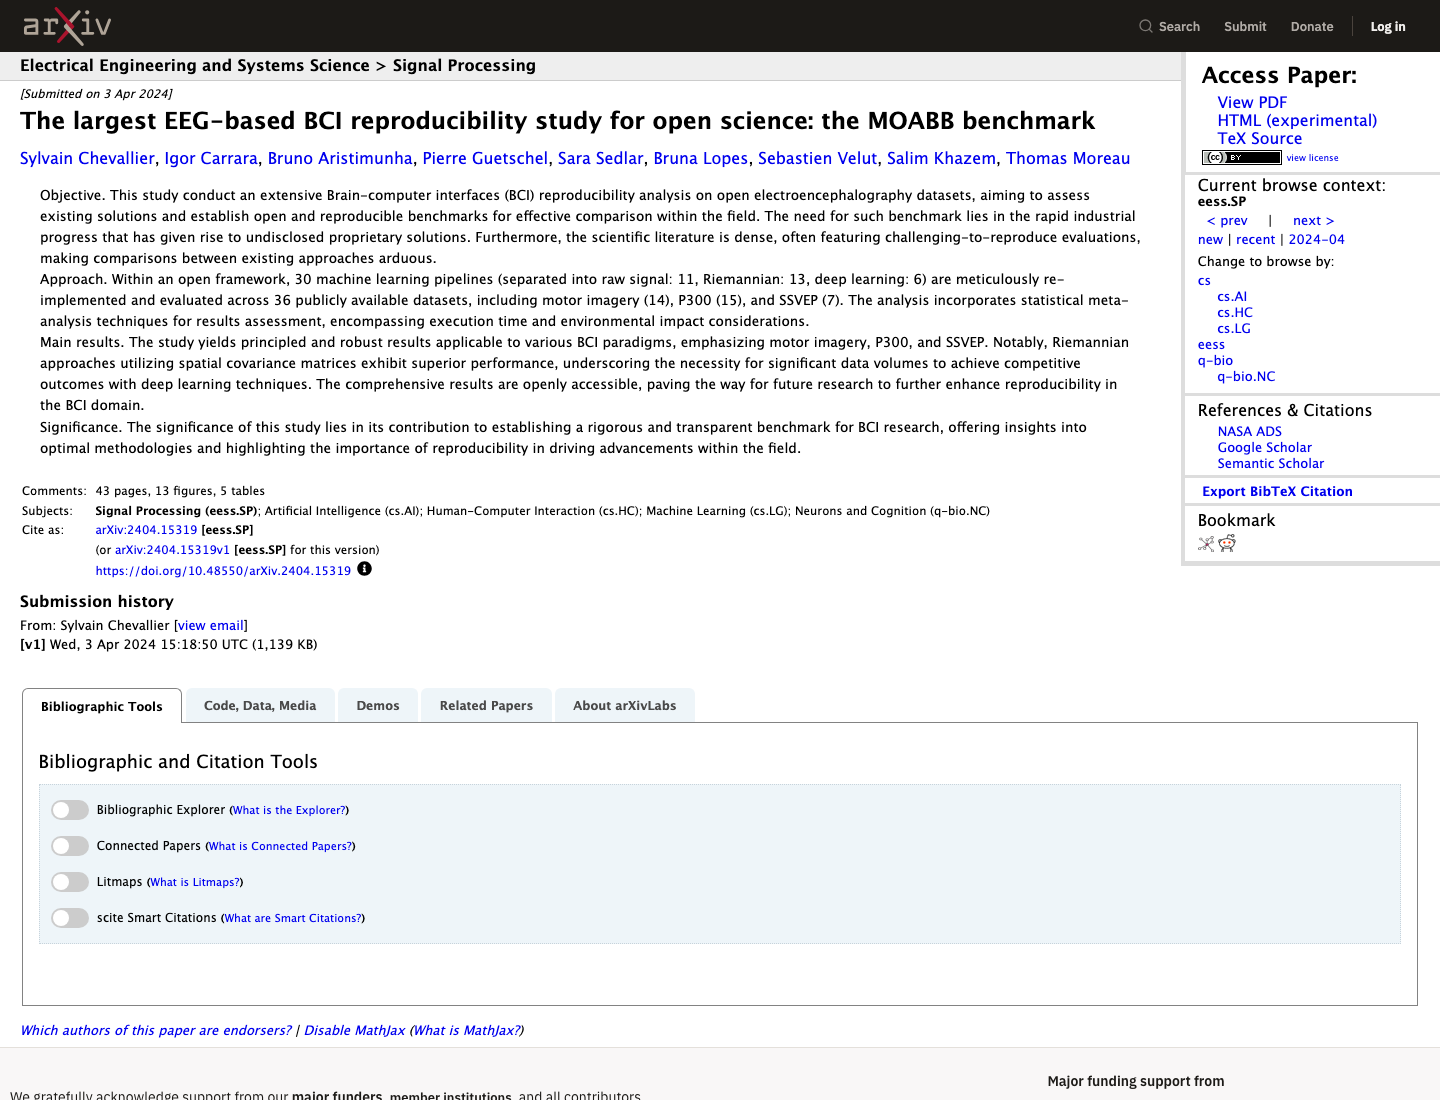
\includegraphics[width=\linewidth,height=45mm,keepaspectratio]{assets/history/moabb-arxiv-abstract.png}
      \par\smallskip{\scriptsize The MOABB benchmark --- arXiv abstract page\par}
  \end{columns}
  \NTXSource{https://arxiv.org/abs/2404.15319}{Chevallier et al., 2024, arXiv:2404.15319}
  
  \note{[13:00--14:00] MOABB makes datasets and comparisons reusable so different people can learn and test results on common ground. The figures refer to the 2024 study, not a current dataset total. Credit the contributors. Better benchmarks are a community asset; they do not by themselves establish clinical utility.}
\end{frame}

\begin{frame}{NeuroTechX\,$\heartsuit$\,DLEEG}
  \framesubtitle{Deep learning for EEG: a community effort}
  \begin{columns}[c,onlytextwidth]
    \column{.54\textwidth}
      \fontsize{9.5}{11}\selectfont
      \NTXPoint{Make the field understandable}{Yannick Roy and colleagues' review: a map of deep learning for EEG and a call for reproducibility.}
      \NTXPoint{Teach with shared tools}{Workshops connect MNE, scikit-learn, pyRiemann, and MOABB; new contributors carry the teaching forward.}
      \NTXPoint{Turn datasets into shared work}{Neureka/TUH, hackathon challenges, and neural foundation models: compare methods and share what works.}
    \column{.42\textwidth}
      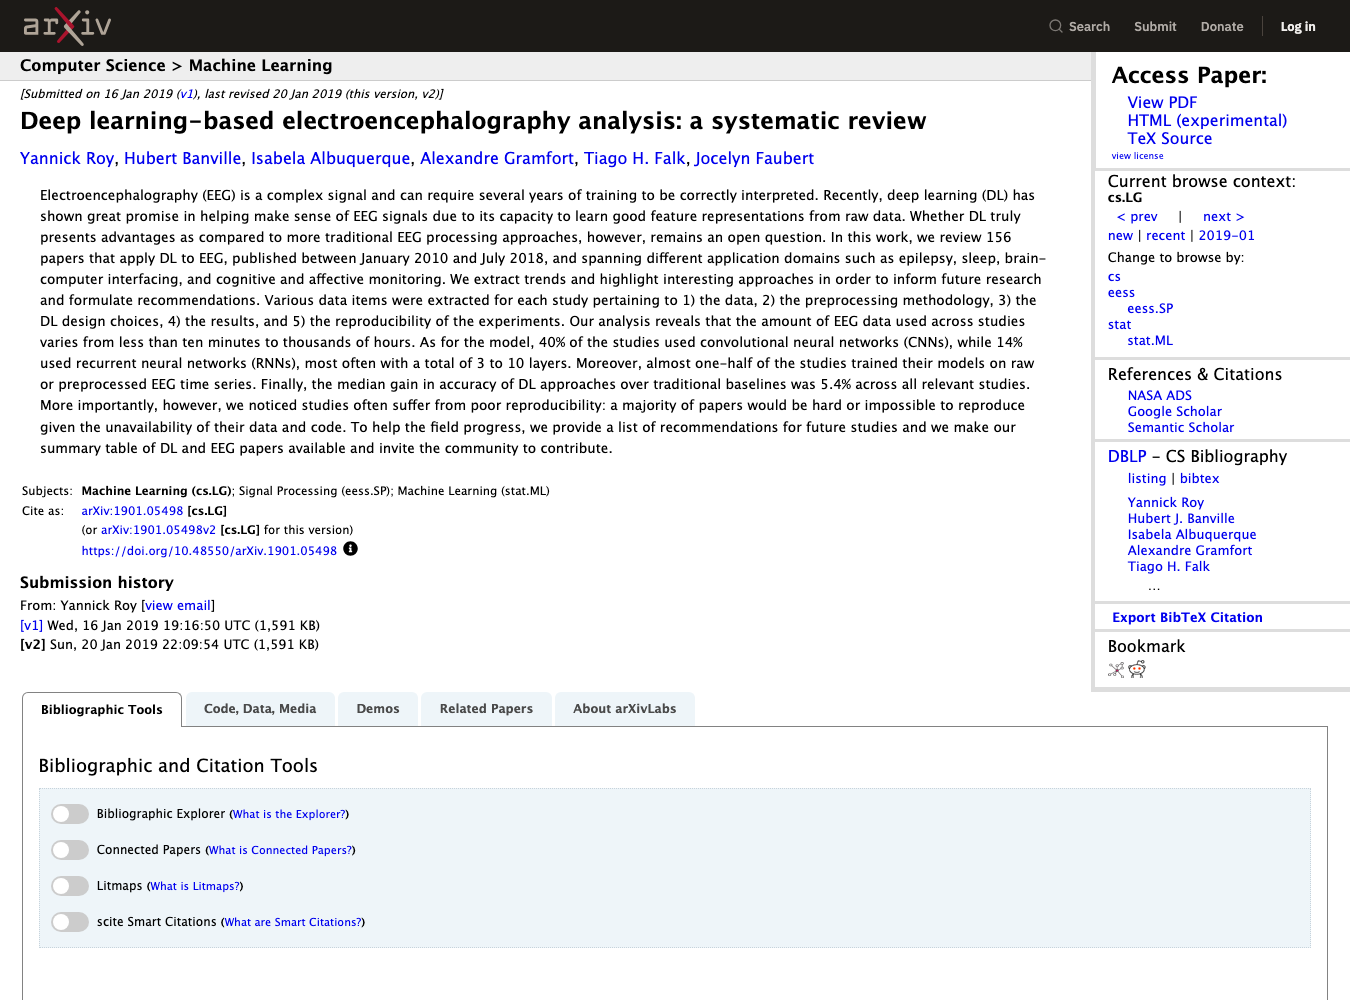
\includegraphics[width=\linewidth,height=43mm,keepaspectratio]{assets/history/dleeg-roy-article-page.png}\par\smallskip
      {\tiny Roy et al., 2019 --- arXiv abstract page\par}
  \end{columns}
  {\tiny\color{NTXMuted}Sources: \href{https://arxiv.org/abs/1901.05498}{Roy et al.}; \href{https://github.com/mccorsi/BCI-2023-Open-Source-Tool-workshop}{open-source BCI workshop}; \href{https://isip.piconepress.com/conferences/ieee_spmb/2020/papers/l02_05.pdf}{Neureka scoring study}\par}
  \note{[14:00--15:00] Summarize the full DLEEG section in one minute. Roy and colleagues synthesized the literature and emphasized sharing data and code. Pedro Rodrigues, Sylvain Chevallier and other contributors taught open-tool workflows, with newer contributors extending that teaching. Neureka joined NeuroTechX, Novela and the Temple TUH corpus team around seizure detection and shared scoring. Not every listed library, challenge or foundation model is an NTX creation, and the challenge was not restricted to deep learning. The connection is community participation through education, shared data, reproducibility and evaluation. Retain classical baselines as models become larger; this is not a claim that deep learning always wins. The detailed full-deck DLEEG slides retain the underlying sources and historical distinctions.}
\end{frame}

\section{Students Are the Future}
\NTXDivider{Students Are the Future}

% Selected from slides.tex
\begin{frame}{A competition that helped organize student clubs}
  \begin{columns}[T,onlytextwidth]
    \column{.49\textwidth}
      \NTXPoint{2016: a five-club pilot}{Montr\'eal and Toronto; a November Demo Day in Montr\'eal.}
      \NTXPoint{A reason to organize}{The annual competition helped students establish university clubs.}
      \NTXPoint{A shared goal}{Build a project and show the work.}
    \column{.46\textwidth}
      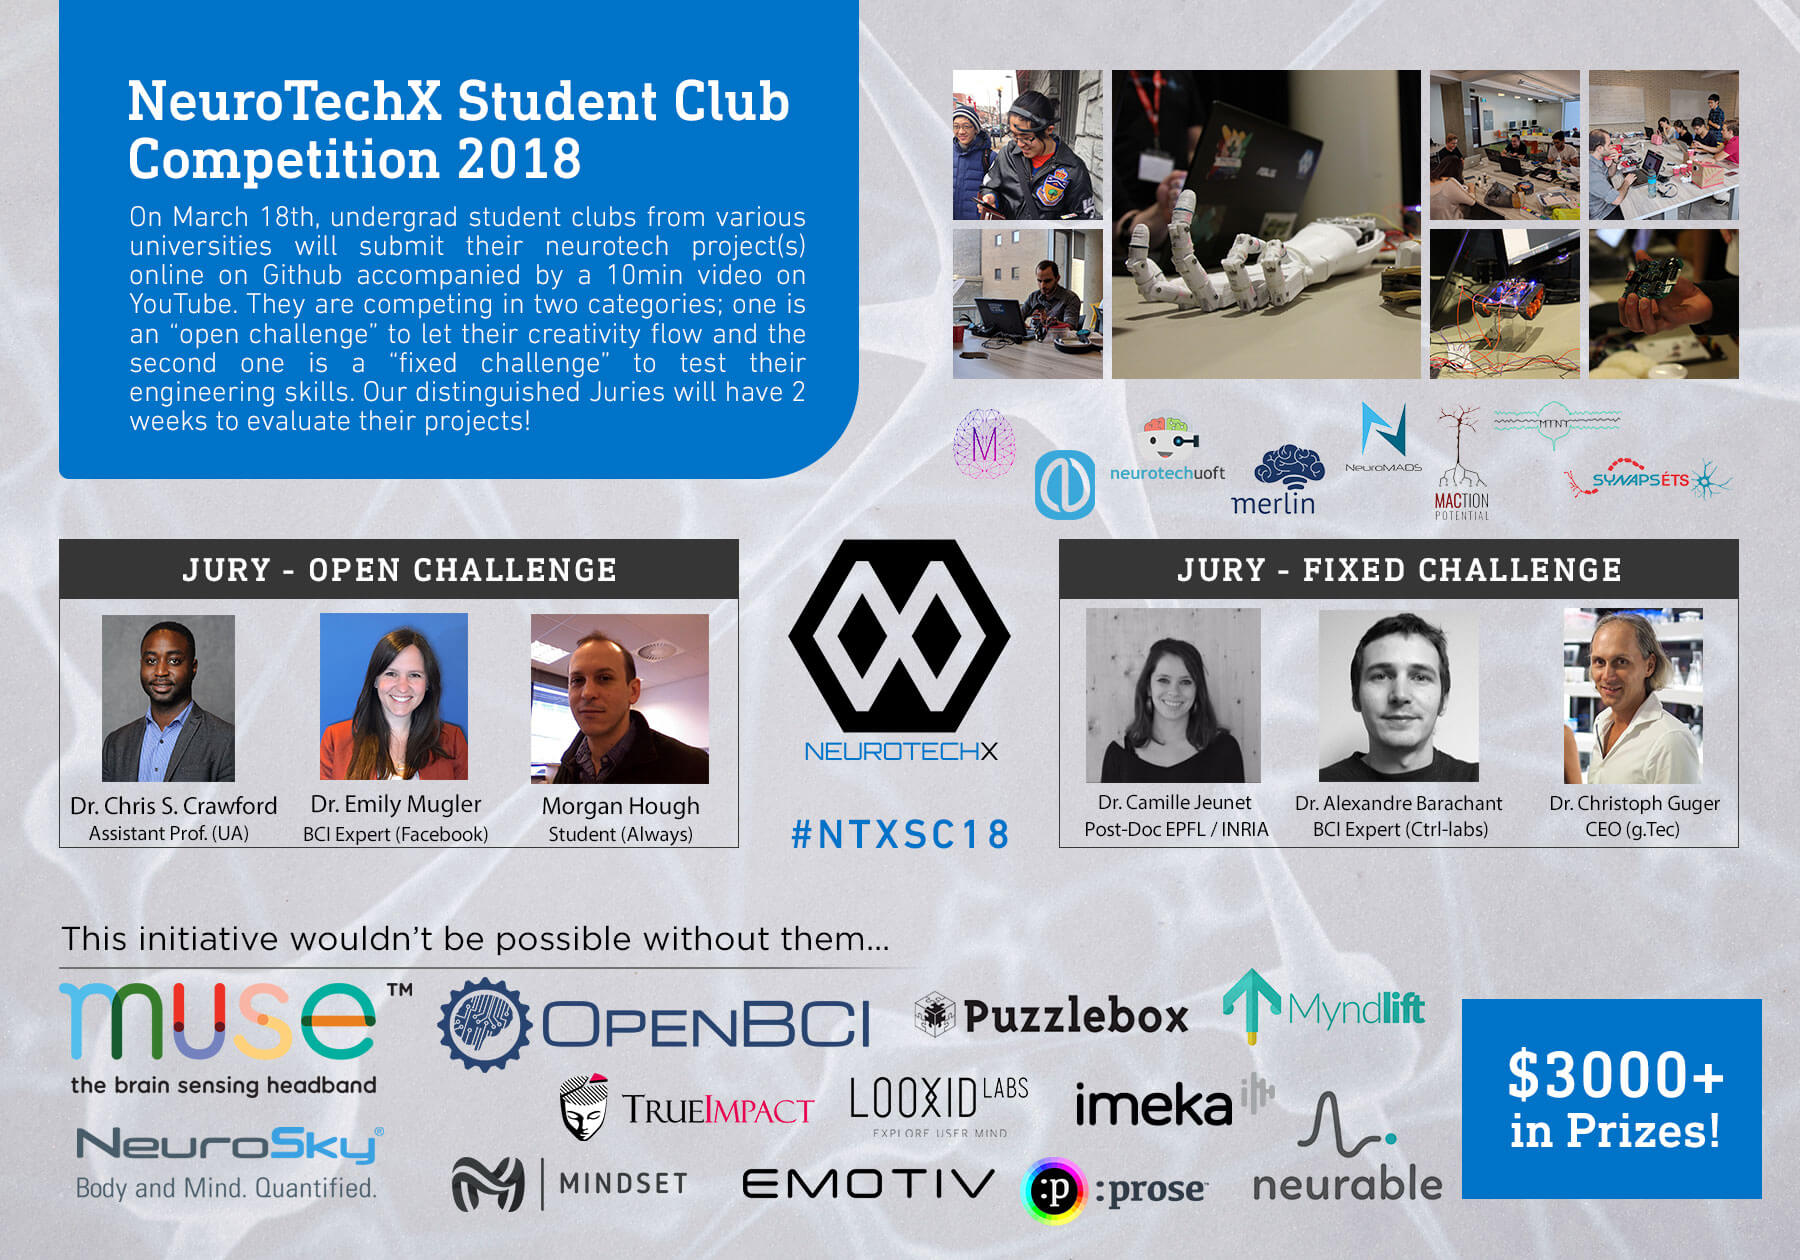
\includegraphics[width=\linewidth,height=44mm,keepaspectratio]{assets/history/student-competition-2018-flyer.jpg}
      \par\smallskip{\scriptsize Original 2018 competition announcement\par}
  \end{columns}
  {\tiny\color{NTXMuted}Sources: \href{https://medium.com/neurotechx/ntx-student-clubs-initiative-2fba98b0d082}{NeuroTechX's 2017 retrospective}; \href{https://neurotechx.com/ntx-student-clubs-competition/}{2018 announcement}\par}
  
  \note{[15:00--16:15] The annual competition became an organizing function for student chapters. The documented five-club 2016 pilot gave people a shared reason to form teams, work through a project and demonstrate it. The displayed flyer is from 2018. Focus on creating recurring reasons to organize, not on prizes alone. No current worldwide student-club count is asserted.}
\end{frame}

% Selected from slides.tex
\begin{frame}{Student participation: people and projects}
  \begin{columns}[c,onlytextwidth]
    \column{.58\textwidth}
      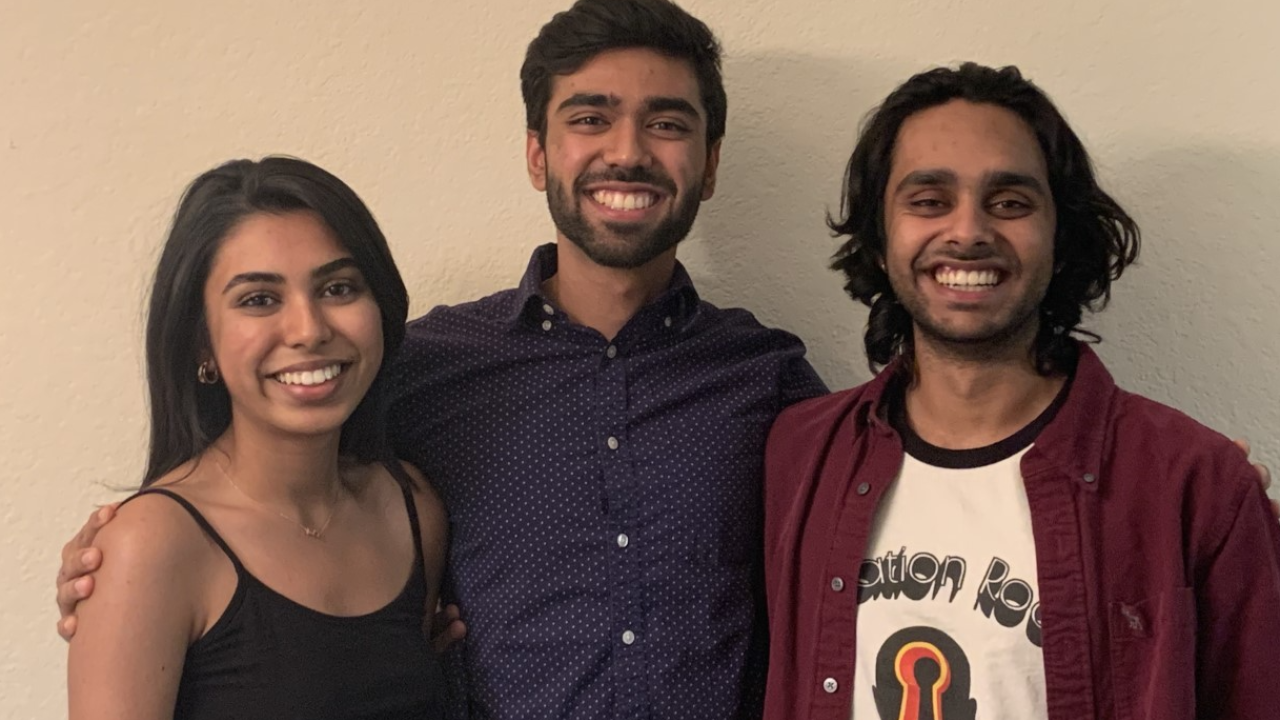
\includegraphics[width=\linewidth,height=37mm,keepaspectratio]{assets/chapters/uc-davis-neuroassist-team-2020.png}
      \par\smallskip{\small Neurotech@Davis: the NeuroAssist team\par}
    \column{.36\textwidth}
      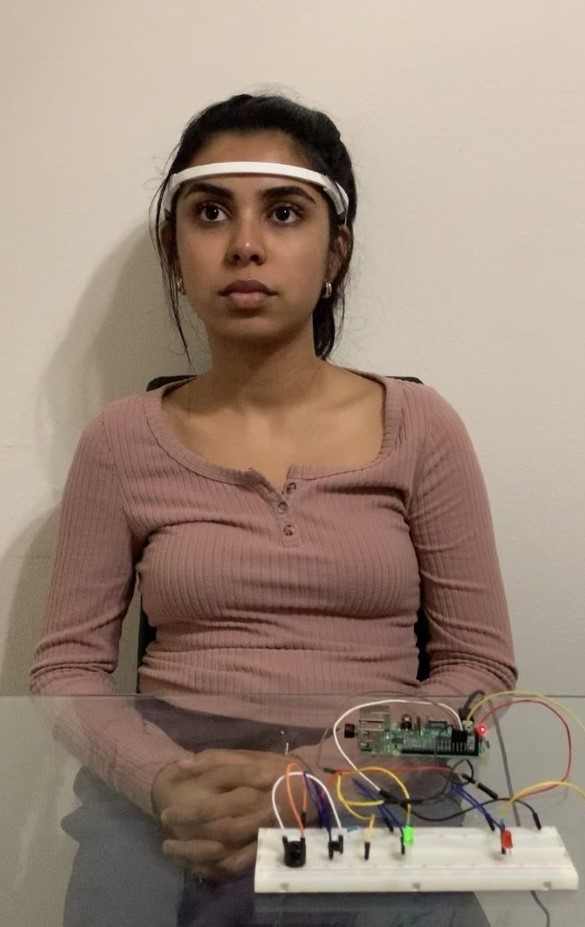
\includegraphics[width=\linewidth,height=37mm,keepaspectratio]{assets/chapters/uc-davis-neuroassist-headset-2020.jpg}
      \par\smallskip{\small Priyanshi wearing NeuroAssist\par}
  \end{columns}
  \medskip
  {\small Built for the 2020 NeuroTechX Student Competition.\par}
  \NTXSource{https://neuroengineering.ucdavis.edu/news/neurotechdavis-student-club-undergraduate-students-learn-about-neurotechnology}{Photos and identification: Neuroengineering at UC Davis, April 2022}
  
  \note{[16:15--17:15] Make the previous idea concrete with Neurotech@Davis and NeuroAssist. UC Davis identifies these photos with the 2020 competition project, in an article published in 2022. The learning is in building and explaining a working project together. Do not present a competition prototype as a clinically validated intervention.}
\end{frame}

% Selected from history/global-neurohack.tex
\begin{frame}{Global NeuroHack 2026}
  \begin{columns}[c,onlytextwidth]
    \column{.43\textwidth}
      \small
      \NTXPoint{April 10--12, 2026}{Frontier Tower, San Francisco.\newline NeuroTechX organizing support.}
      \NTXPoint{Three tracks}{Blue-Sky Prototyping; Non-Implantable Speech Decoding; Maximizing Bit Rate.}
      \NTXPoint{From ideas to presentations}{Workshops, mentor check-ins, and project demos.}
    \column{.53\textwidth}
      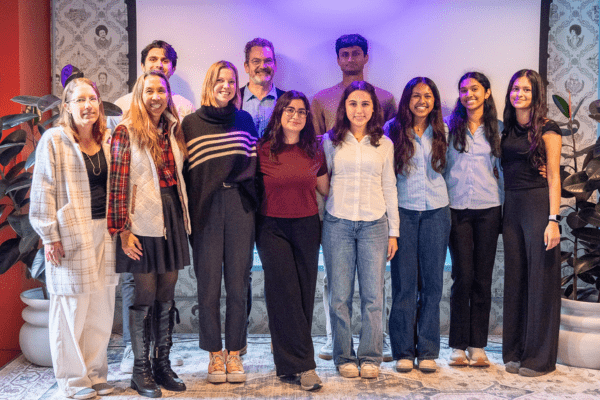
\includegraphics[width=\linewidth,height=43mm,keepaspectratio]{assets/chapters/ucsc-global-neurohack-winners-2026.png}
      \par\smallskip{\scriptsize UCSC's NeuroBite team with judges\newline Blue Sky Track winners\par}
  \end{columns}
  {\tiny\color{NTXMuted}Sources: \href{https://global-neurohack.github.io/}{Global NeuroHack 2026}; photo / team identification: \href{https://engineering.ucsc.edu/news/ucsc-students-win-global-neurohack-2026/}{UC Santa Cruz / Baskin Engineering, June 8, 2026}\par}

  \note{[17:15--18:45] Move from local student teams to cross-community collaboration. Morgan hosted and supported the April event at Frontier Tower. UCSC's report identifies five first-year NeuroTechSC students as Blue Sky Track winners with NeuroBite. Describe this as a track award, not sole winners of the event. Use Morgan's firsthand perspective on mentoring and participation; do not invent turnout or subsequent startup outcomes. The student-club logo graphic requested earlier is still unavailable and is not replaced by sponsor logos.}
\end{frame}

% Selected from slides.tex
\begin{frame}{The NeuroTech Microcredential Program}
  \begin{columns}[T,onlytextwidth]
    \column{.62\textwidth}
      \NTXPoint{2022: partnership announced}{Queen's Centre for Neuroscience Studies and NeuroTechX; Ontario-funded development.}
      \NTXPoint{2024--2025: hands-on capstones}{First cohort: May 2024. Second: August 2025.\newline 15 students in each cohort.}
      \NTXPoint{Online learning into lab practice}{Neuroscience, recording, imaging, and ethics;\newline a two-week, team-based capstone.}
    \column{.33\textwidth}
      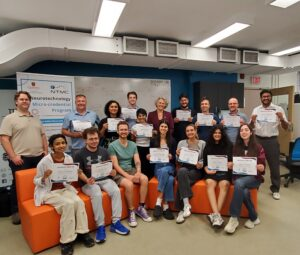
\includegraphics[width=\linewidth]{assets/history/queens-capstone-2025.jpg}
      \par\smallskip{\scriptsize 2025 capstone cohort\par}
  \end{columns}
  {\tiny\color{NTXMuted}Sources: \href{https://www.queensu.ca/gazette/media/news-release-queen-s-micro-credentials-address-knowledge-gaps-burgeoning-neurotech-industry}{Queen's launch announcement, October 2022}; \href{https://neurotechmicrocreds.com/capstone/}{program history and cohort photo}\par}
  
  \note{[18:45--20:00] Explain a more structured education route. Queen's announced its NTX partnership in October 2022; the program documents 15 students in each of its 2024 and 2025 capstones. Students combined instruction with project design, data collection, analysis and presentations. The pictured cohort is 2025. The lesson is a practical progression from learning to team work, not a claim of current NTX governance or guaranteed employment.}
\end{frame}

\section{The Next Neurotech Founders}
\NTXDivider{The Next Neurotech Founders}

% Selected from future.tex
\begin{frame}{McGill NeuroTech: student-built TMS research hardware}
  \begin{columns}[c,onlytextwidth]
    \column{.57\textwidth}
      \small
      \NTXPoint{A new hardware-team preprint}{Lapatrie and collaborators: a low-cost monophasic transcranial magnetic stimulator.}
      \NTXPoint{About US\$700 in parts}{Off-the-shelf components and a custom coil; bench equipment is additional.}
      \NTXPoint{Build, characterize, share}{Measured magnetic fields inform cortical-field models. A concrete example of ambitious student research.}
      {\scriptsize Research prototype --- not approved for human stimulation or clinical use.\par}
    \column{.39\textwidth}
      \centering
      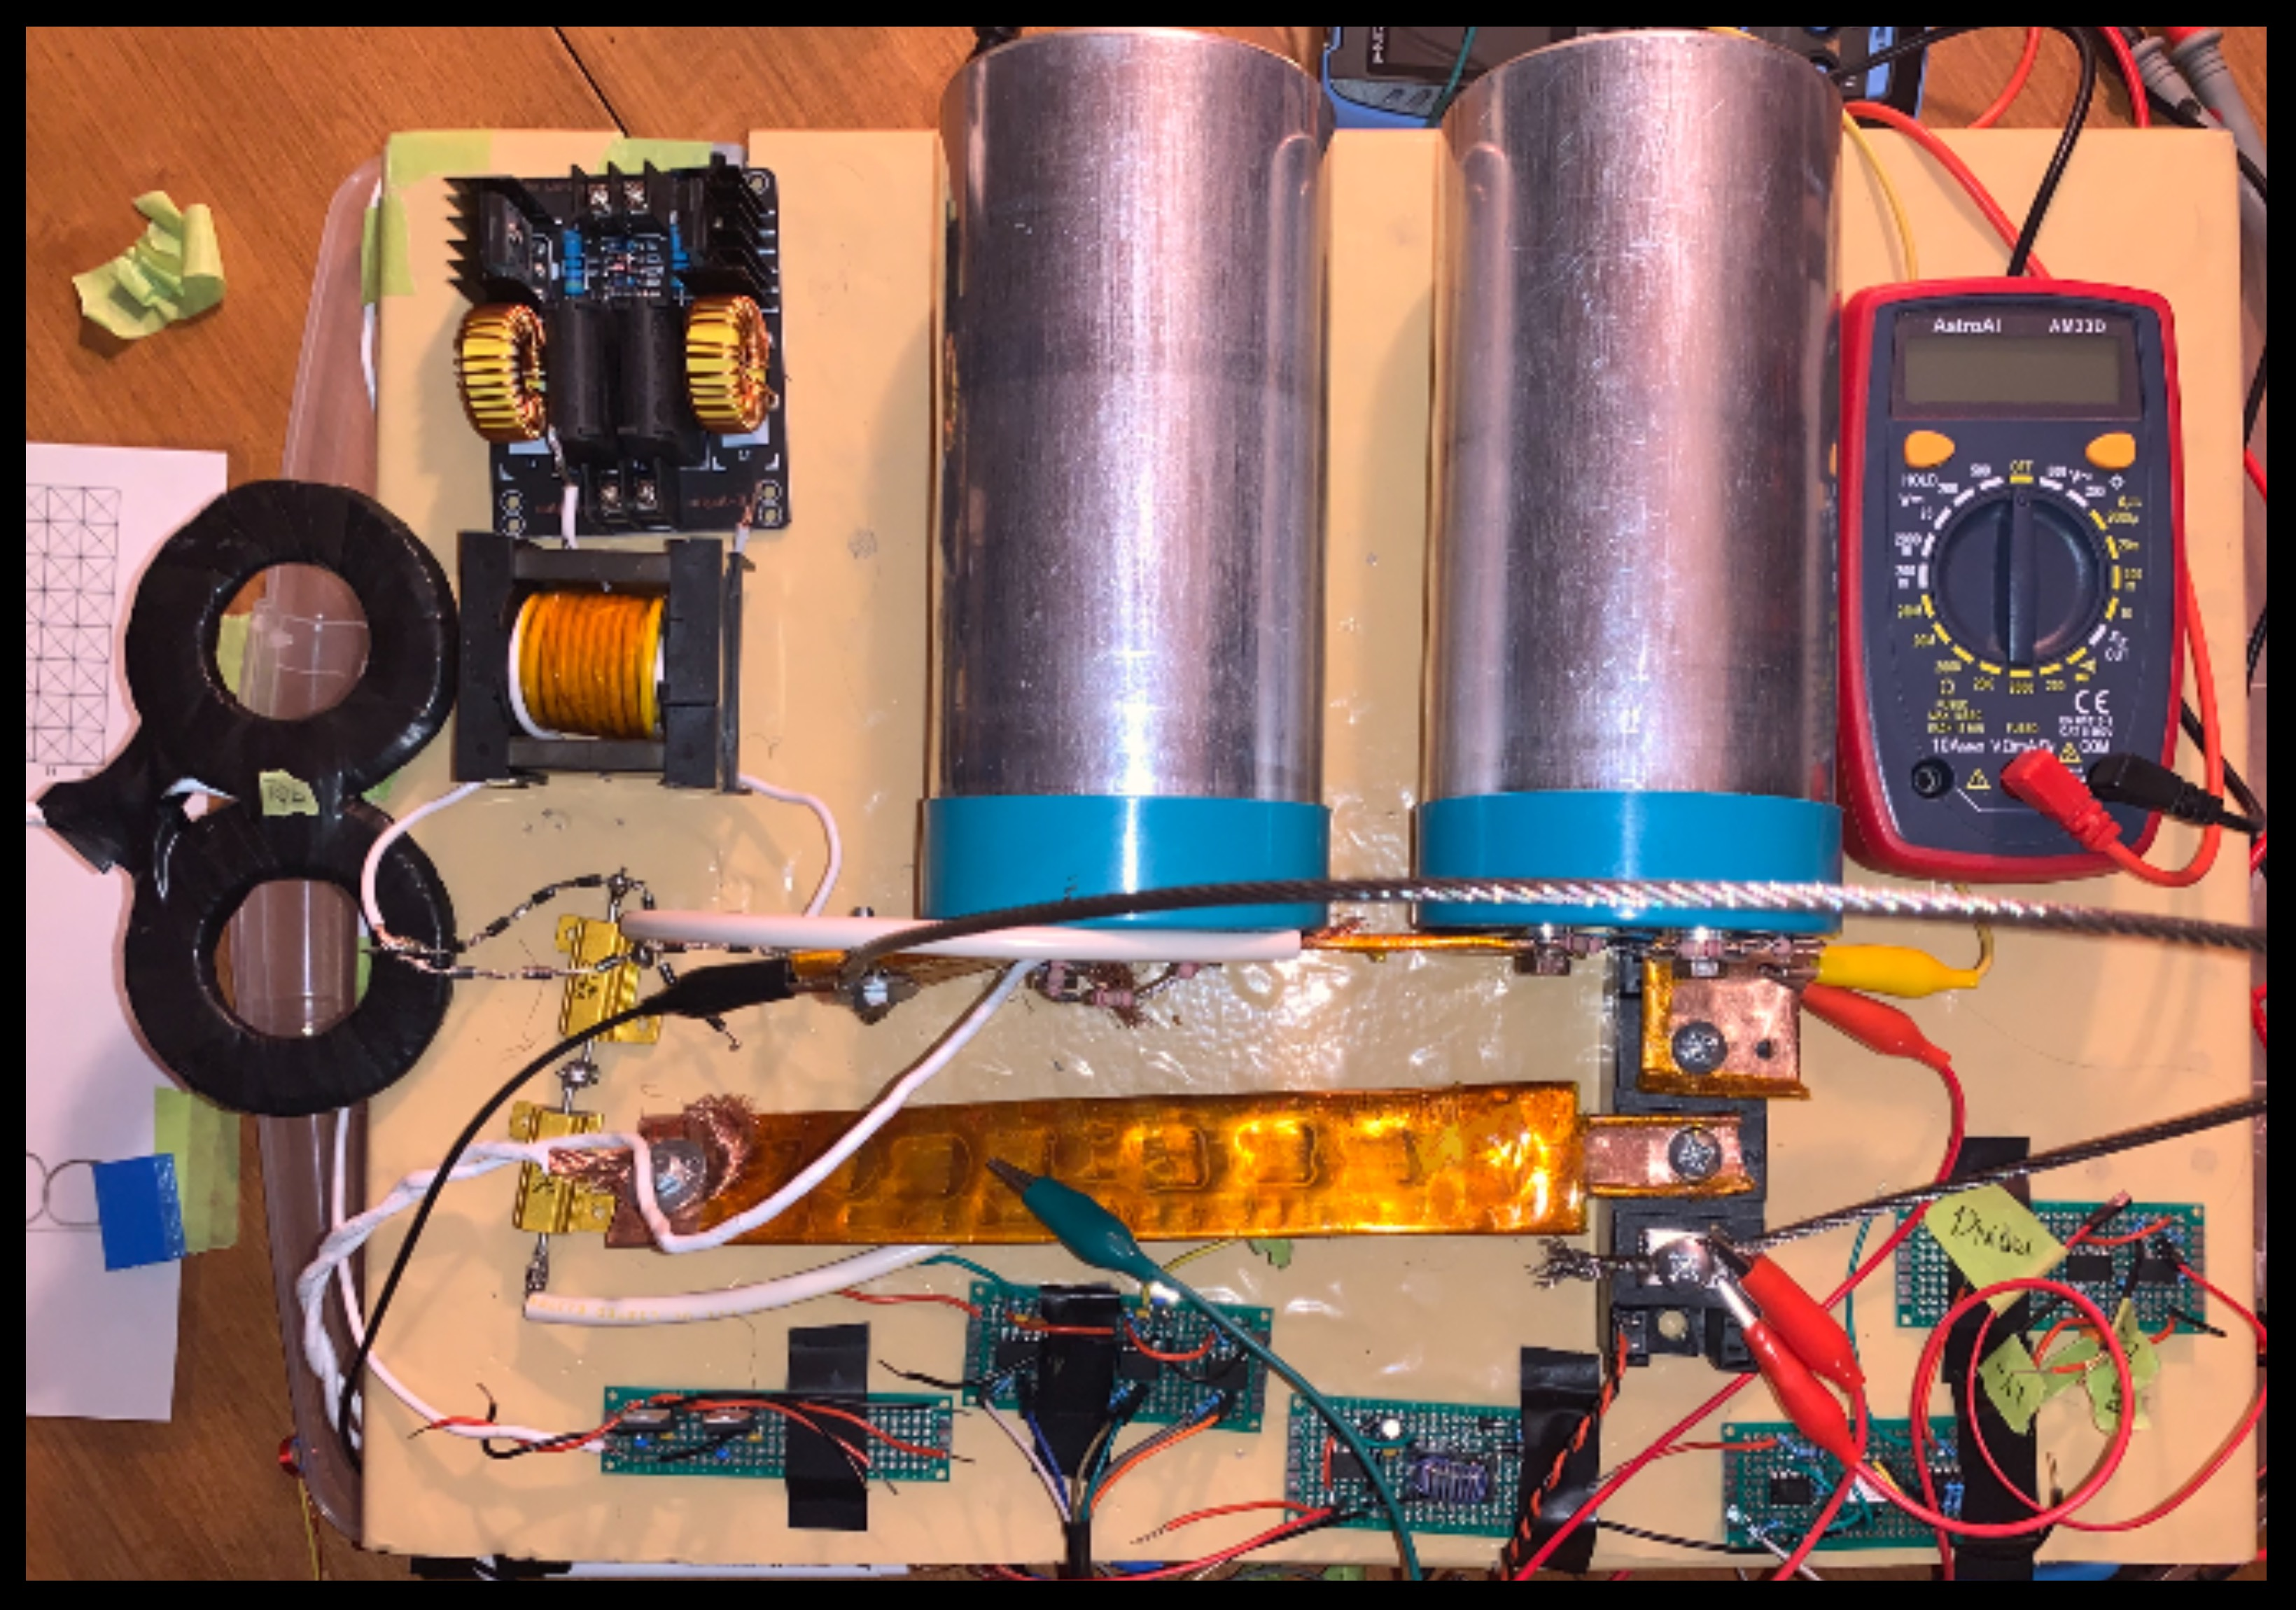
\includegraphics[width=\linewidth,height=23mm,keepaspectratio]{assets/history/mcgill-tms-prototype.jpg}
      \par{\tiny Prototype --- top view\par}\smallskip
      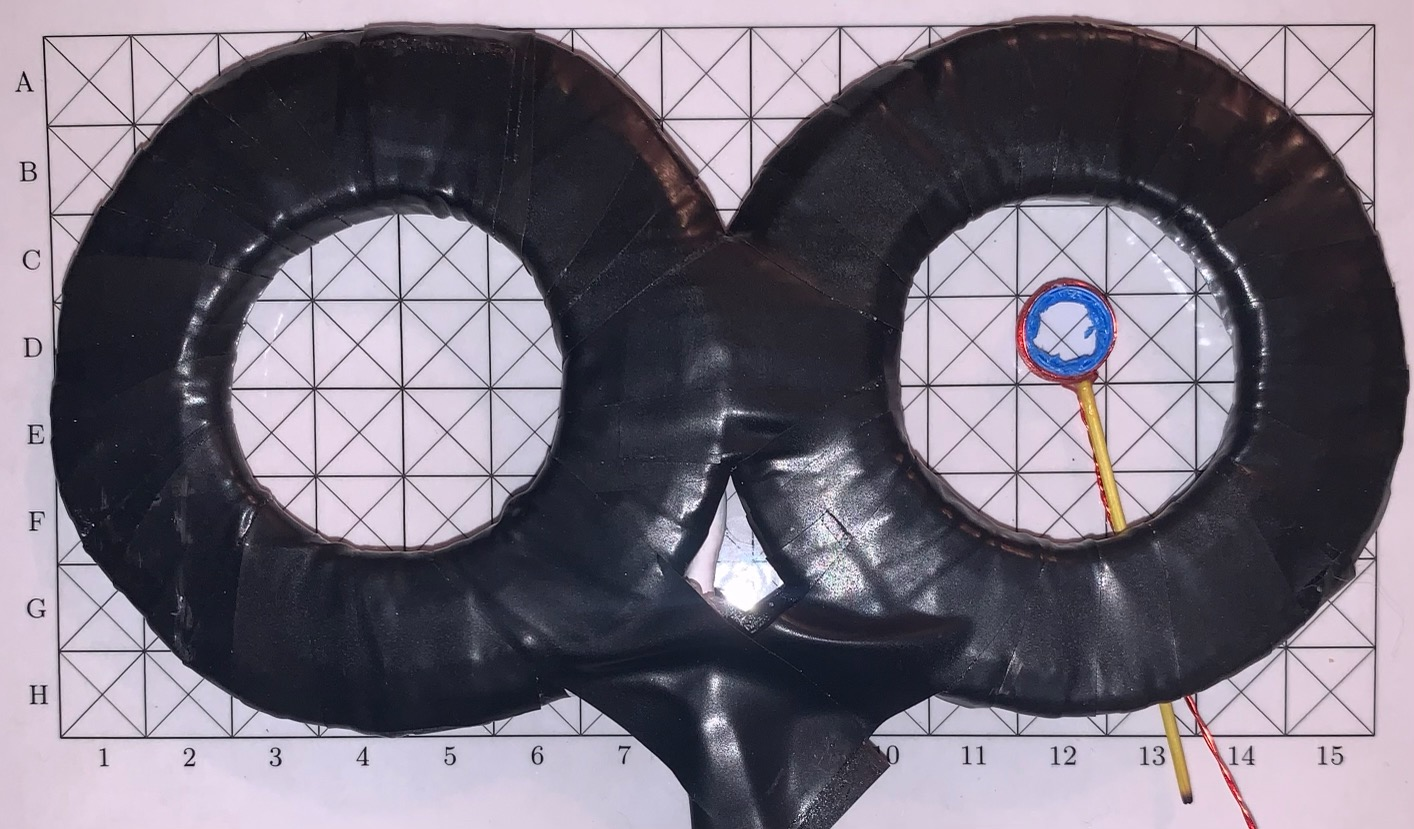
\includegraphics[width=\linewidth,height=21mm,keepaspectratio]{assets/history/mcgill-tms-coil.jpg}
      \par{\tiny Coil and field-measurement setup\par}
  \end{columns}
  {\tiny\color{NTXMuted}Sources: \href{https://www.linkedin.com/posts/maxence-lapatrie_brain-stimulation-research-can-be-expensive-activity-7498376586744709120-7w6N}{team announcement}; \href{https://doi.org/10.64898/2026.08.25.747050}{bioRxiv, August 2026}; photos: \href{https://www.mcgill.ca/ose/files/ose/2-35_-_maxence.pdf}{McGill project poster}\par}
  
  \note{[20:00--21:15] Use one ambitious student project: McGill's TMS hardware and characterization. The preprint reports about USD700 in parts, excluding assumed bench equipment. It is research hardware, explicitly not approved for human stimulation or clinical use. Student opportunity includes measurement, simulation and reproducibility, not self-treatment. The poster image predates the latest preprint; do not compare their cost tables as if they were the same revision.}
\end{frame}

% Selected from future.tex
\begin{frame}{Build an MRI: Johns Hopkins, September 16--18}
  \begin{columns}[c,onlytextwidth]
    \column{.50\textwidth}
      \small
  \NTXPoint{Coming up: DELTA DIY-MRI 2026}{Three days at Johns Hopkins University in Baltimore: learn, design, build, and scan.}
  \NTXPoint{A mentored, hands-on team project}{Build low-field MRI components and image a phantom: magnets, RF and gradient coils, acquisition, and reconstruction.}
  \NTXPoint{Free attendance; currently sold out}{Join the waitlist, or explore the public build resources and community.}
    \column{.46\textwidth}
      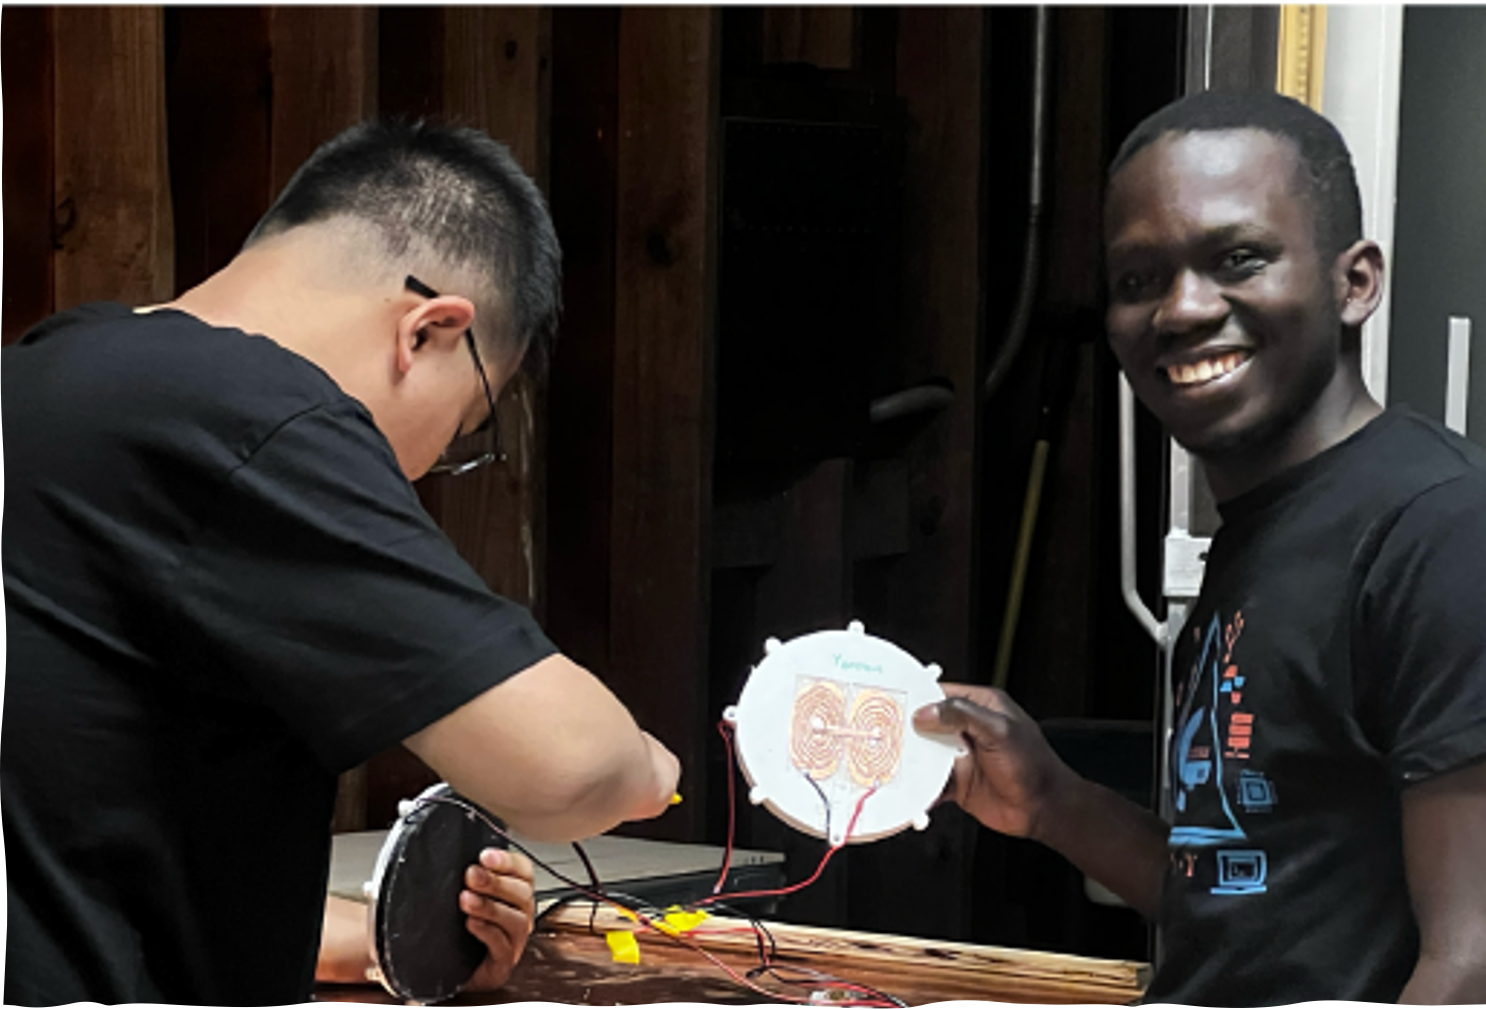
\includegraphics[width=\linewidth,height=42mm,keepaspectratio]{assets/history/jhu-diy-mri-build.png}\par\smallskip
      {\scriptsize Earlier workshop: hands-on building\newline Photo: DELTA DIY-MRI organizers\par}
  \end{columns}
  \NTXSource{https://delta-diy-mri.github.io/}{delta-diy-mri.github.io --- September 16--18, 2026; waitlist and resources}
  
  \note{[21:15--22:15] An immediate external opportunity: DELTA DIY-MRI at Johns Hopkins, September 16--18, 2026, nine days after this presentation. Free attendance but currently sold out, with a waitlist. Public build resources and the community are also available. The photo is from an earlier workshop. The program uses mentored construction and phantom imaging, not human scanning; it is not an NTX event.}
\end{frame}
\begin{frame}{The second wave: Neuralink and new founders}
  \begin{columns}[c,onlytextwidth]
    \column{.43\textwidth}
      \fontsize{9.5}{11}\selectfont
      \NTXPoint{Implants enter the public conversation}{Elon Musk and Neuralink brought new attention to BCI and how to participate.}
      \NTXPoint{The conversation expands}{From headsets to implants, clinical development, and neurotech careers.}
      \NTXPoint{Our role}{Turn curiosity into informed learning, useful projects, and grounded expectations.}
    \column{.53\textwidth}
      \fontsize{9.5}{11}\selectfont
      \textbf{Neuralink co-founders, subsequent ventures}\par\medskip
      Max Hodak $\longrightarrow$ \textbf{Science Corporation}\par\medskip
      Benjamin Rapoport $\longrightarrow$ \textbf{Precision Neuroscience}\par\medskip
      Philip Sabes $\longrightarrow$ \textbf{Starfish Neuroscience}\par\bigskip
      {\scriptsize A broader set of approaches, not one technical path. Starfish's research includes non-invasive neuromodulation and distributed implantable interfaces.\par}
  \end{columns}
  \smallskip{\scriptsize\color{NTXMuted}The bridge to a third wave: more routes into the brain, more functions to explore.\par}
  {\tiny\color{NTXMuted}Founder links: \href{https://science.xyz/company/team/max-hodak/}{Science}; \href{https://www.precisionneuro.io/our-vision}{Precision}; \href{https://profiles.ucsf.edu/philip.sabes}{UCSF / Sabes}. \href{https://starfishneuroscience.com/research/}{Starfish research}. Community shift: Morgan's experience.\par}
  \note{[23:15--24:45] Neuralink did not invent BCI: BrainGate and other implant research predated it. Morgan describes how the public visibility of Elon Musk and Neuralink changed the questions and ambitions people brought to the community; this is qualitative experience, not a measured membership or funding effect. Three verified founder paths illustrate a widening ecosystem: Max Hodak co-founded Neuralink and founded Science; Benjamin Rapoport co-founded Neuralink and Precision; Philip Sabes helped build Neuralink's founding team and co-founded Starfish in 2020. These are independent companies, not asserted corporate spin-offs or exclusive founder lists. Sabes's UCSF profile now also describes work on Integral Neurotechnologies; do not imply he still leads Starfish. Starfish explicitly researches non-invasive TMS and distributed implantable interfaces. These are distinct approaches, not proof of a fully non-invasive multi-region system. Founders' subsequent ventures illustrate diversification, not evidence that Neuralink caused every later innovation. Use this as the historical bridge to the emerging third-wave direction; these waves overlap.}
\end{frame}

\begin{frame}{A third wave of BCI: non-invasive, multi-target}
  \framesubtitle{An emerging direction}
  \begin{columns}[c,onlytextwidth]
    \column{.56\textwidth}
      \fontsize{9.5}{11}\selectfont
      \NTXPoint{Beyond one signal, one function}{Combine distributed signals and context; aim for multiple useful readouts, not only a single control task.}
      \NTXPoint{Neural foundation models (NeuroFMs)}{Shared representations across recordings, regions, and tasks are becoming a research tool.}
      \NTXPoint{Non-invasive routes remain central}{BrainOmni learns across EEG and MEG; POYO+ demonstrates multi-task transfer in mouse imaging.}
    \column{.40\textwidth}
      \centering
      {\small\textbf{The opportunity}\par}\smallskip
      \fbox{\parbox{.86\linewidth}{\centering\small Distributed neural signals\\+ behavioral context}}
      \par\smallskip $\downarrow$ \par\smallskip
      \fbox{\parbox{.86\linewidth}{\centering\small Shared representation}}
      \par\smallskip $\downarrow$ \par\smallskip
      {\small Multiple task-specific readouts\par}
      \medskip{\tiny Conceptual direction, not a validated product\par}
  \end{columns}
  \smallskip{\scriptsize\color{NTXMuted}Opportunity for the community: open data, strong baselines, and reproducible cross-person evaluation.\par}
  {\tiny\color{NTXMuted}Sources: \href{https://arxiv.org/abs/2505.18185}{BrainOmni, NeurIPS 2025}; \href{https://poyo-plus.github.io/}{POYO+, ICLR 2025}; \href{https://doi.org/10.1038/s41586-025-09235-0}{IBL brain-wide map, Nature 2025}\par}
  \note{[24:45--25:45] Historical framing: consumer headsets brought people together; the second wave renewed implant visibility, including Neuralink; the third points toward non-invasive, multi-target functionality. These waves overlap. Multi-target here means distributed neural sources and multiple functional readouts, not demonstrated multi-site stimulation. NeuroFMs means neural foundation models broadly. Keep the evidence separate: IBL found distributed sensory, choice, movement and reward correlates in mouse Neuropixels recordings; this was not a foundation-model study. POYO+ learned representations transferable across regions and cell types with multiple decoding tasks in mouse two-photon imaging, not non-invasive human BCI. BrainOmni provides the EEG/MEG example, with downstream and cross-device evaluation. Together they motivate the conceptual diagram; they do not establish one integrated, general-purpose real-time BCI. Complex behavior remains constrained by signal quality, context and training data. Community contributions include open data, reproducibility, classical baselines and held-out-person tests. Consent and neural-data privacy matter. Detailed research boundaries and links are in INTRO-JAPAN-2026.md.}
\end{frame}


% Selected from future.tex
\begin{frame}{Biopunk Lab: a home for synthetic neurobiology}
  \begin{columns}[c,onlytextwidth]
    \column{.49\textwidth}
      \small
      \NTXPoint{Back in San Francisco}{Founding Member of Biopunk Lab, working on synthetic neurobiology.}
      \NTXPoint{A place for hands-on work}{Cell culture facility for Neurotech@Berkeley's wetware group.}
      \NTXPoint{Community enables experiments}{Supporting replication work inspired by Mind in Vitro and DishBrain research.}
    \column{.47\textwidth}
      \centering
      
\includegraphics[height=17mm]{assets/history/biopunk-logo.png}
      \par\medskip
      \begin{minipage}[c]{.40\linewidth}
        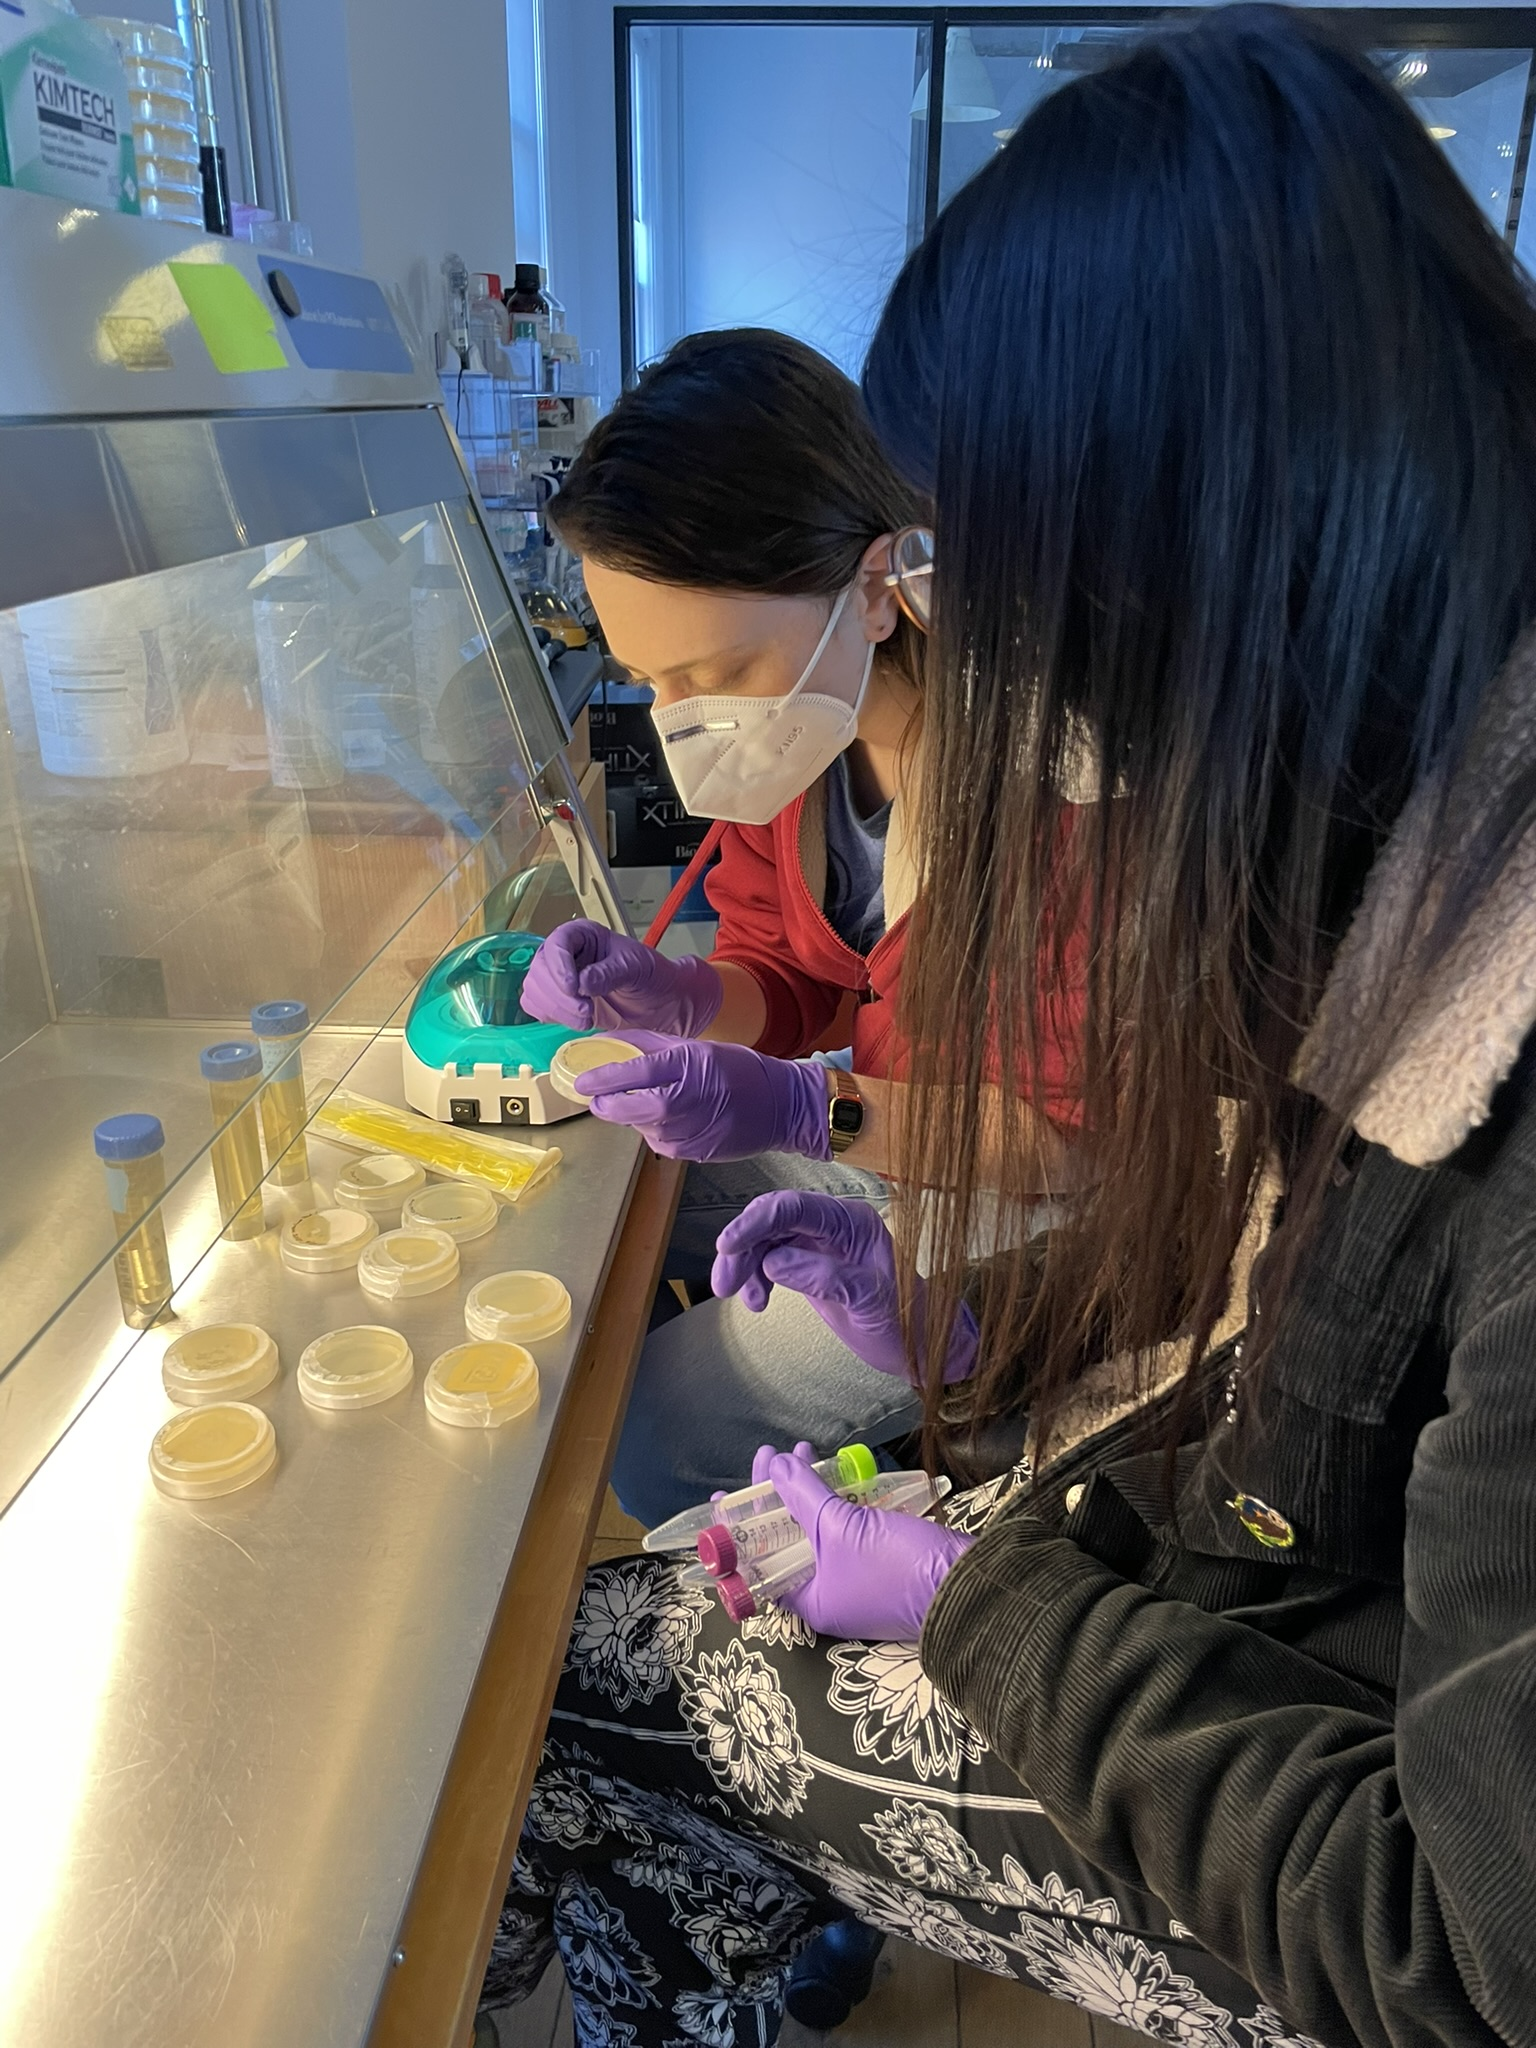
\includegraphics[width=\linewidth,height=31mm,keepaspectratio]{assets/history/biopunk-biosafety.jpeg}
      \end{minipage}\hfill
      \begin{minipage}[c]{.57\linewidth}
        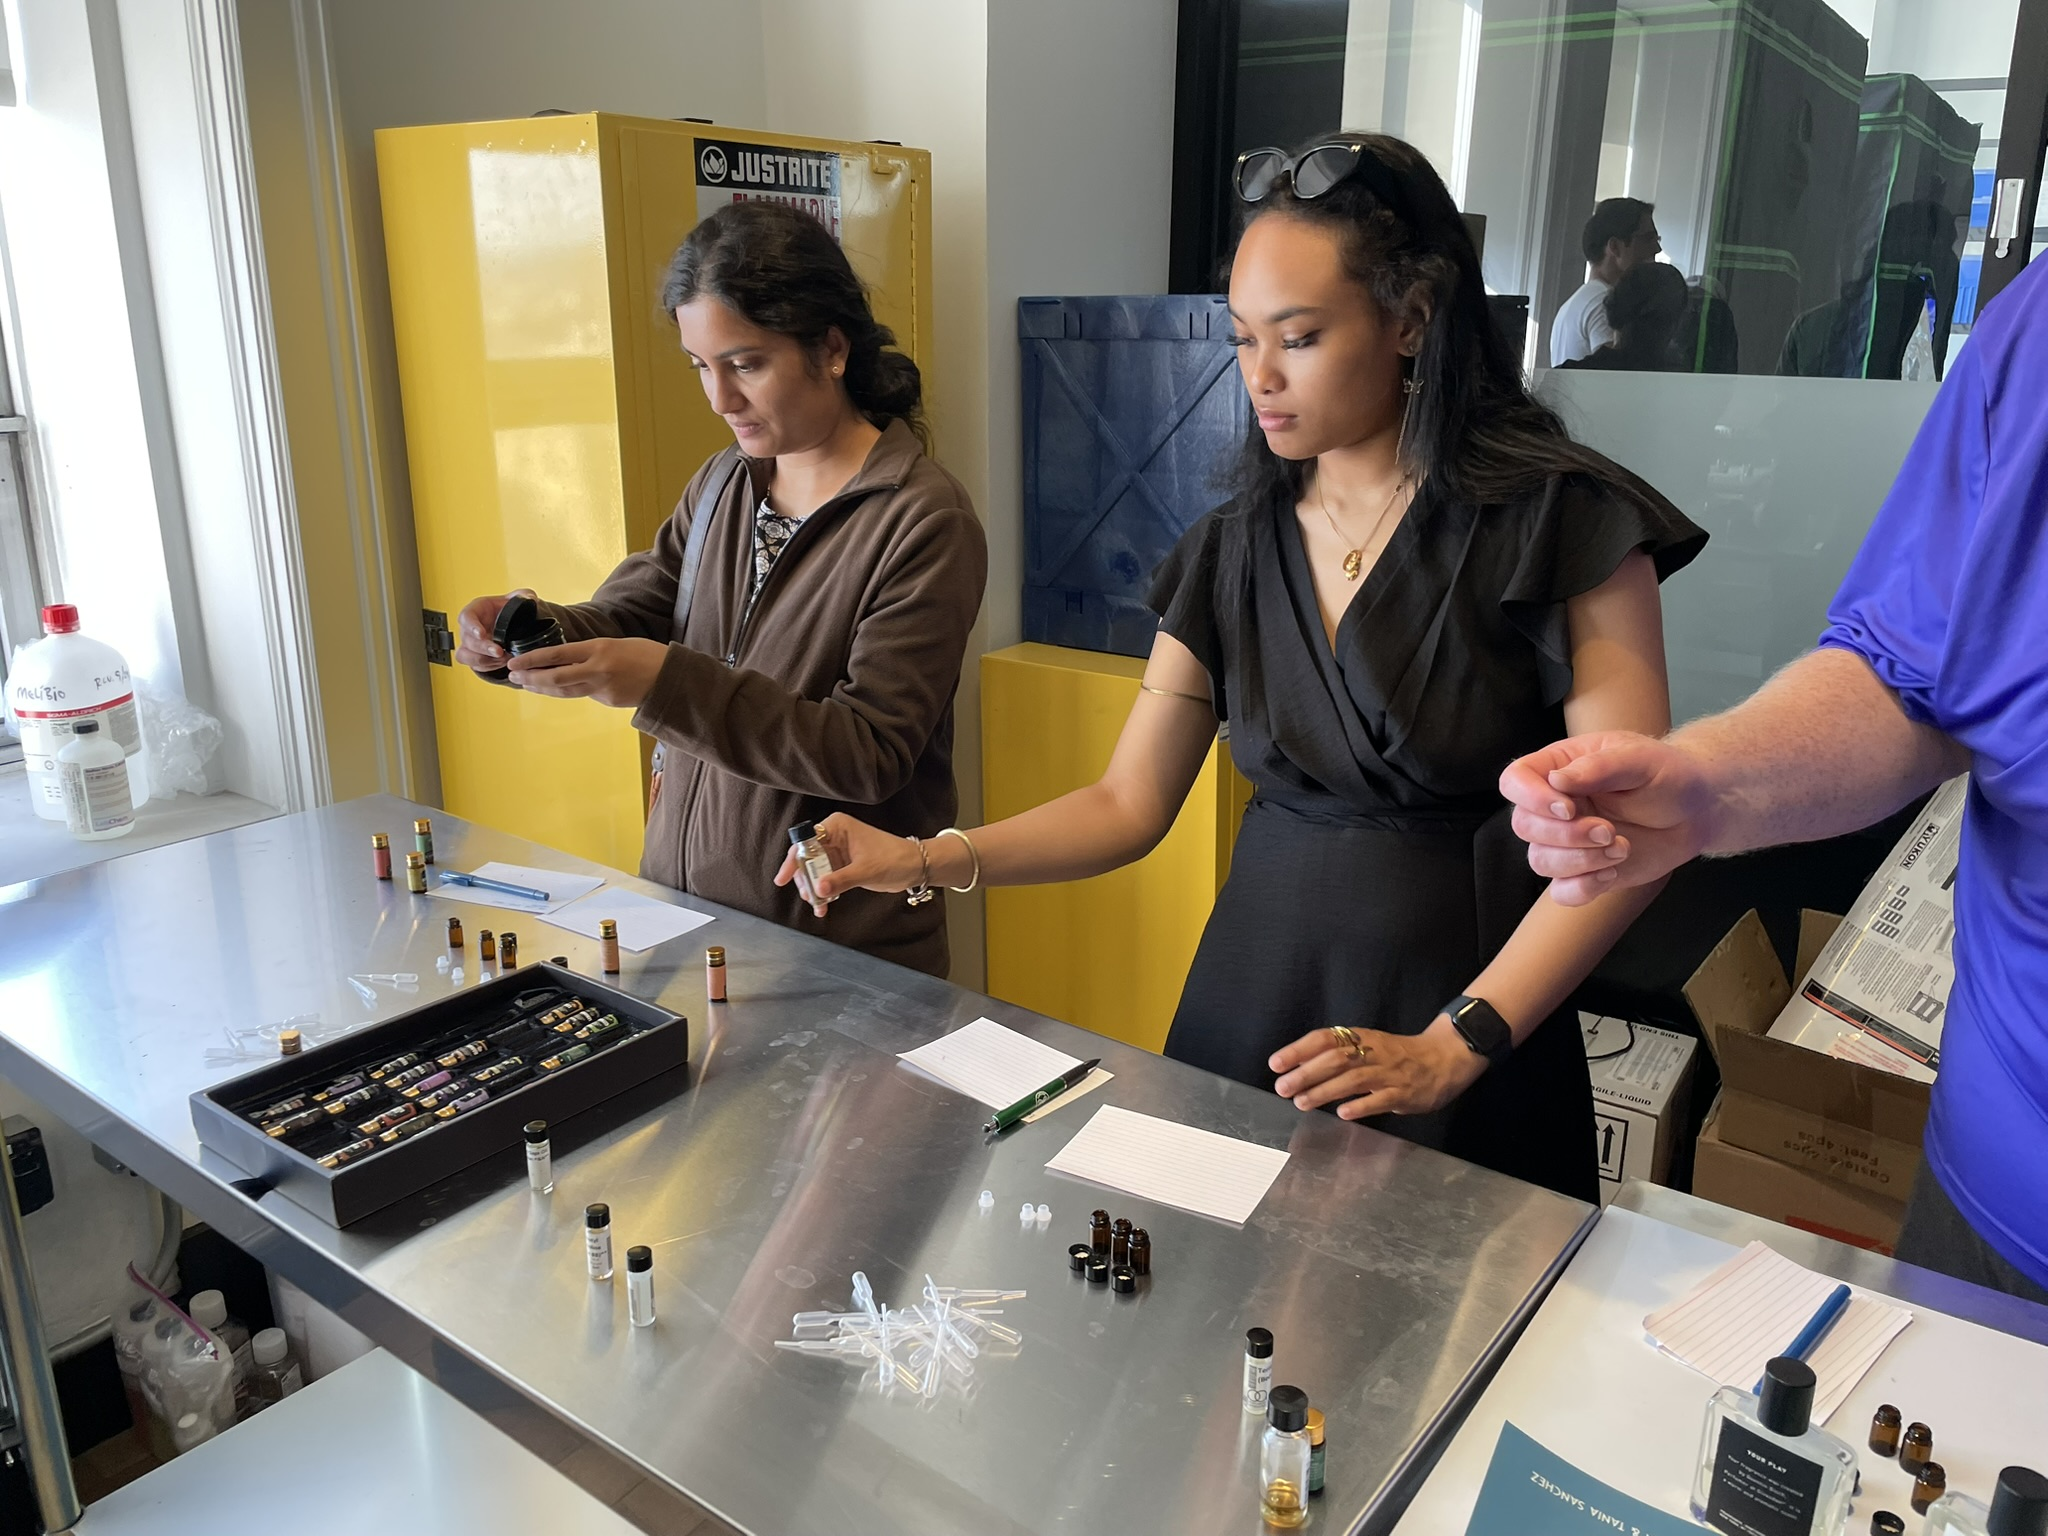
\includegraphics[width=\linewidth,height=31mm,keepaspectratio]{assets/history/biopunk-workshop.jpeg}
      \end{minipage}
      \par\smallskip{\scriptsize Lab work and community workshop\par}
  \end{columns}
  {\tiny\color{NTXMuted}Activities: Morgan Hough's firsthand account. Photos and logo: \href{https://biopunklab.com/}{Biopunk Lab}\par}
  \note{[24:45--25:45] Bring the future discussion back to a physical community lab. Morgan is a founding member working on synthetic neurobiology and reports that Neurotech@Berkeley's wetware group uses Biopunk Lab as its cell culture facility. Describe replication efforts inspired by Mind in Vitro and DishBrain, not completed replication or demonstrated learning results. Those are distinct research projects, not interchangeable names for one experiment. Facilities, mentors, biosafety and ethical oversight matter. The photographs show lab work and a workshop, with the official Biopunk Lab logo. This is another way students can gain access to more ambitious research with appropriate supervision.}
\end{frame}

% Selected from slides.tex
\begin{frame}{What would make these ambitions possible?}
  \begin{columns}[c,onlytextwidth]
    \column{.50\textwidth}
      \small
  \NTXPoint{Access to facilities and mentors}{Help students work beyond the equipment available in a typical club.}
  \NTXPoint{Projects that survive a competition}{Documentation, reproducible tests, and a handover to the next cohort.}
  \NTXPoint{A route to the next experiment}{Keep promising teams connected to collaborators and research opportunities.}
    \column{.46\textwidth}
      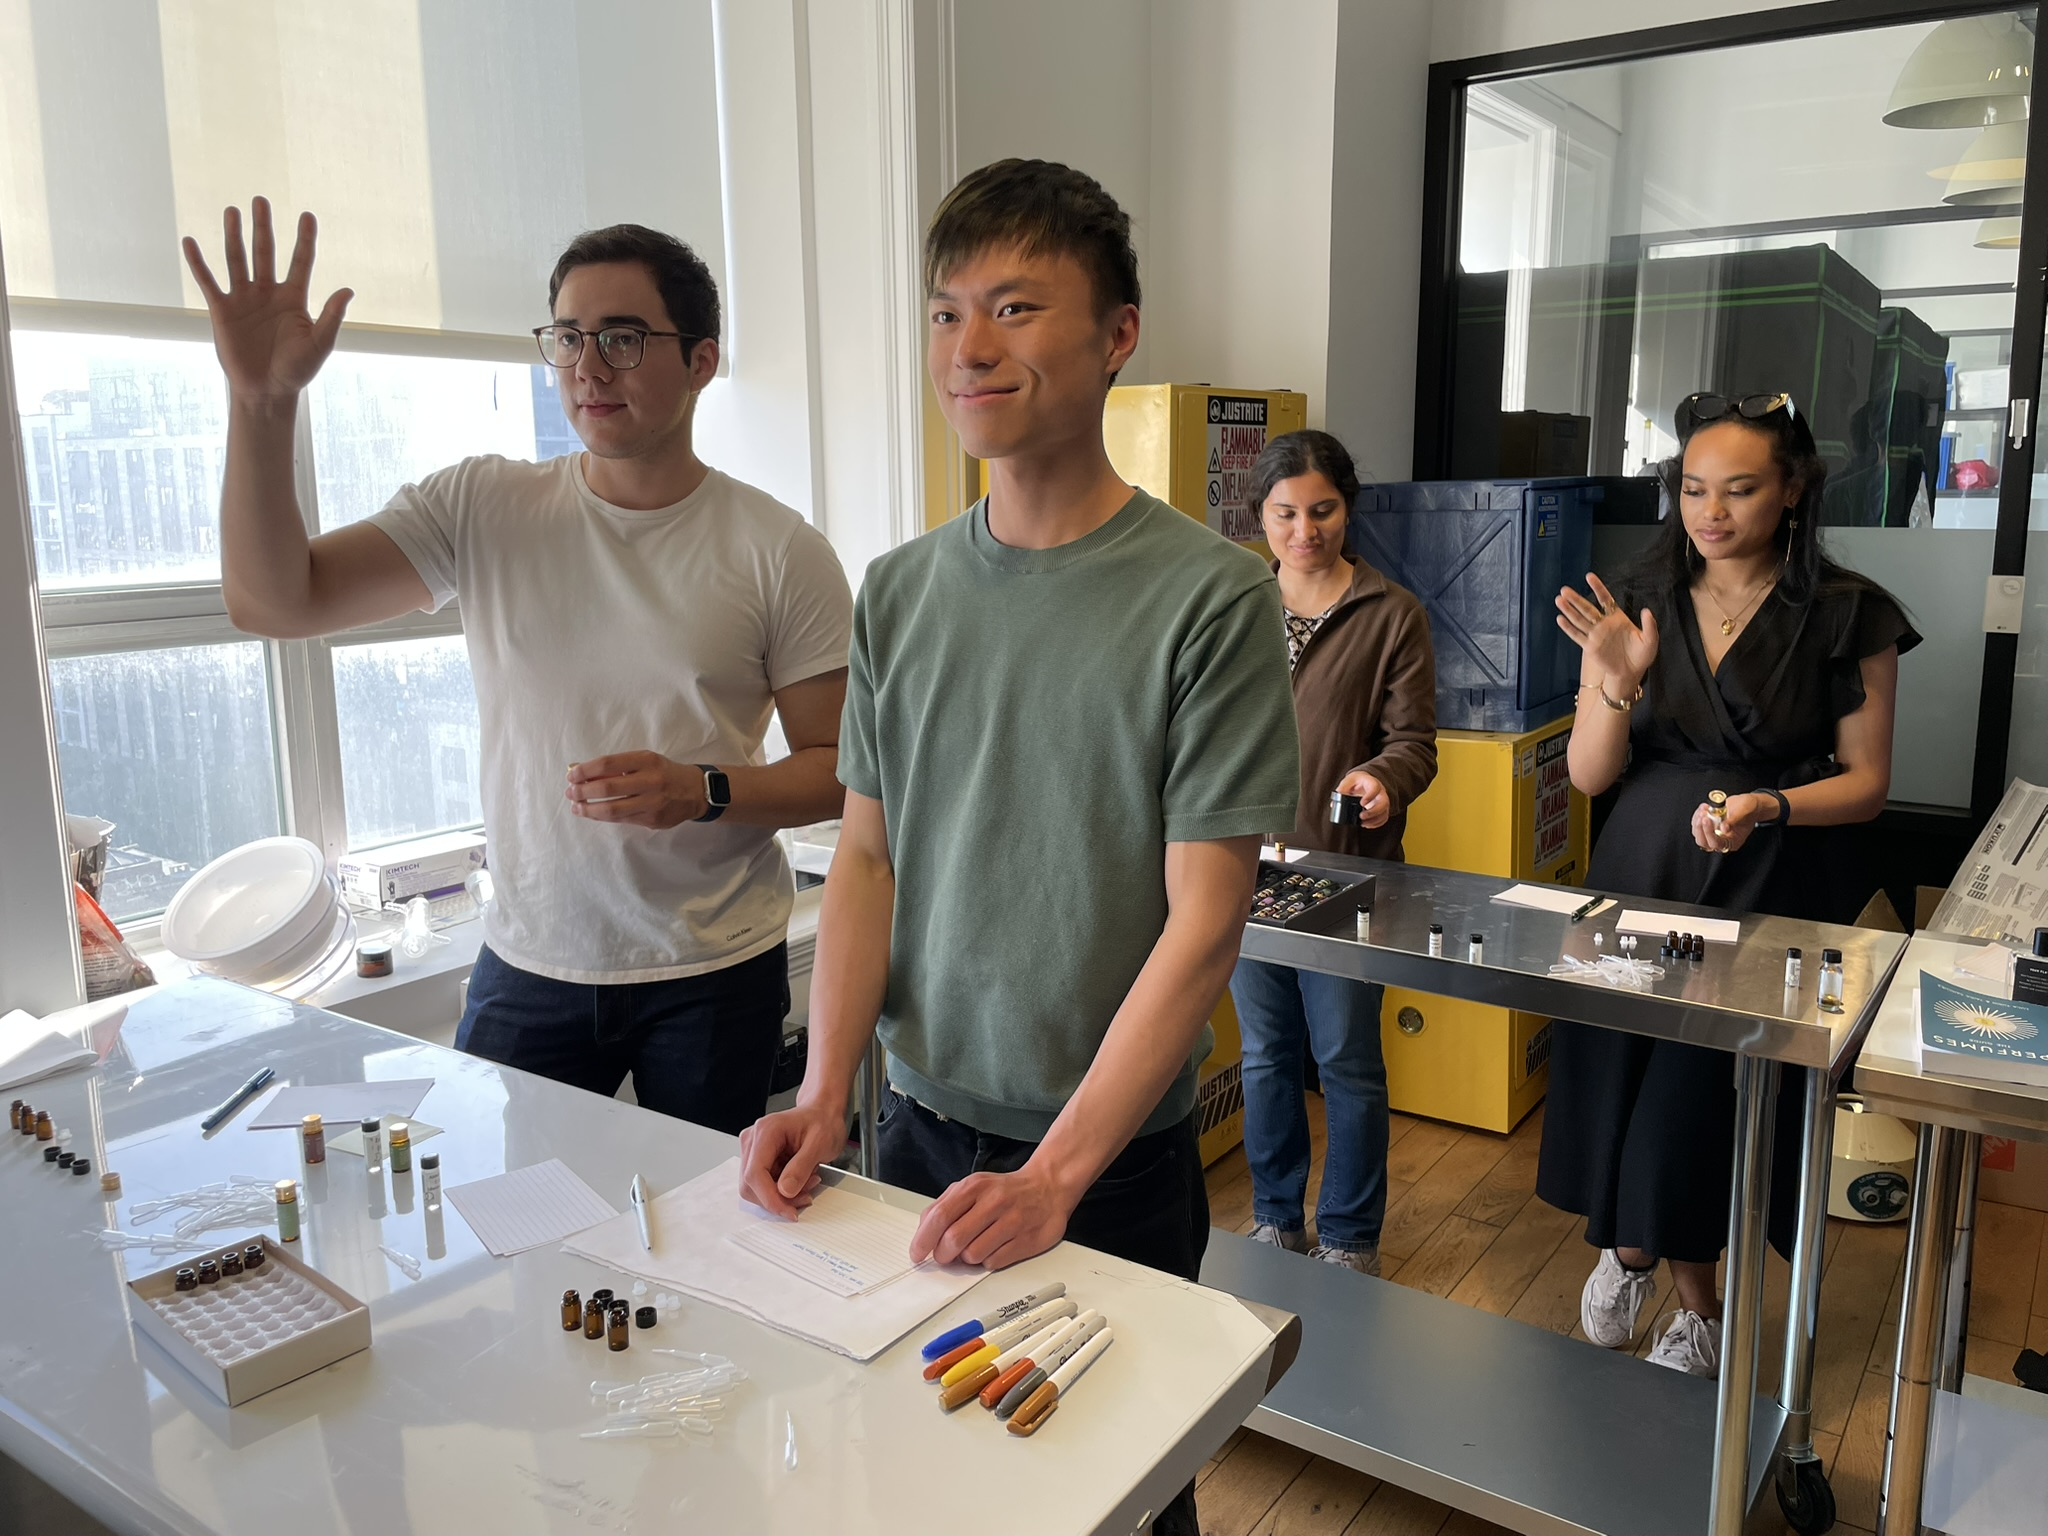
\includegraphics[width=\linewidth,height=44mm,keepaspectratio]{assets/history/biopunk-workshop-2.jpeg}\par\smallskip
      {\scriptsize Facilities and people to learn with\newline Photo: \href{https://biopunklab.com/}{Biopunk Lab}\par}
  \end{columns}
  
  \note{[25:45--27:15] Bring the future discussion back to the community. Morgan's proposed priorities are access to mentors and facilities, documented projects that survive student turnover, and a route to the next experiment. These are priorities to work toward, not promises that access or funding is already secured. For Japan, invite existing labs, makerspaces and university groups to contribute a bounded project, expertise or equipment access.}
\end{frame}

% Selected from slides.tex
\begin{frame}{A founder can also be a community contributor}
  \begin{columns}[c,onlytextwidth]
    \column{.50\textwidth}
      \small
  \NTXPoint{Bring a question people can work on}{A technical problem, an experiment, or a result to examine together.}
  \NTXPoint{Share something useful}{Documentation, a reproducible example, a workshop, or time helping another builder.}
  \NTXPoint{Build relationships through the work}{Meet people by learning, making, and contributing alongside them.}
    \column{.46\textwidth}
      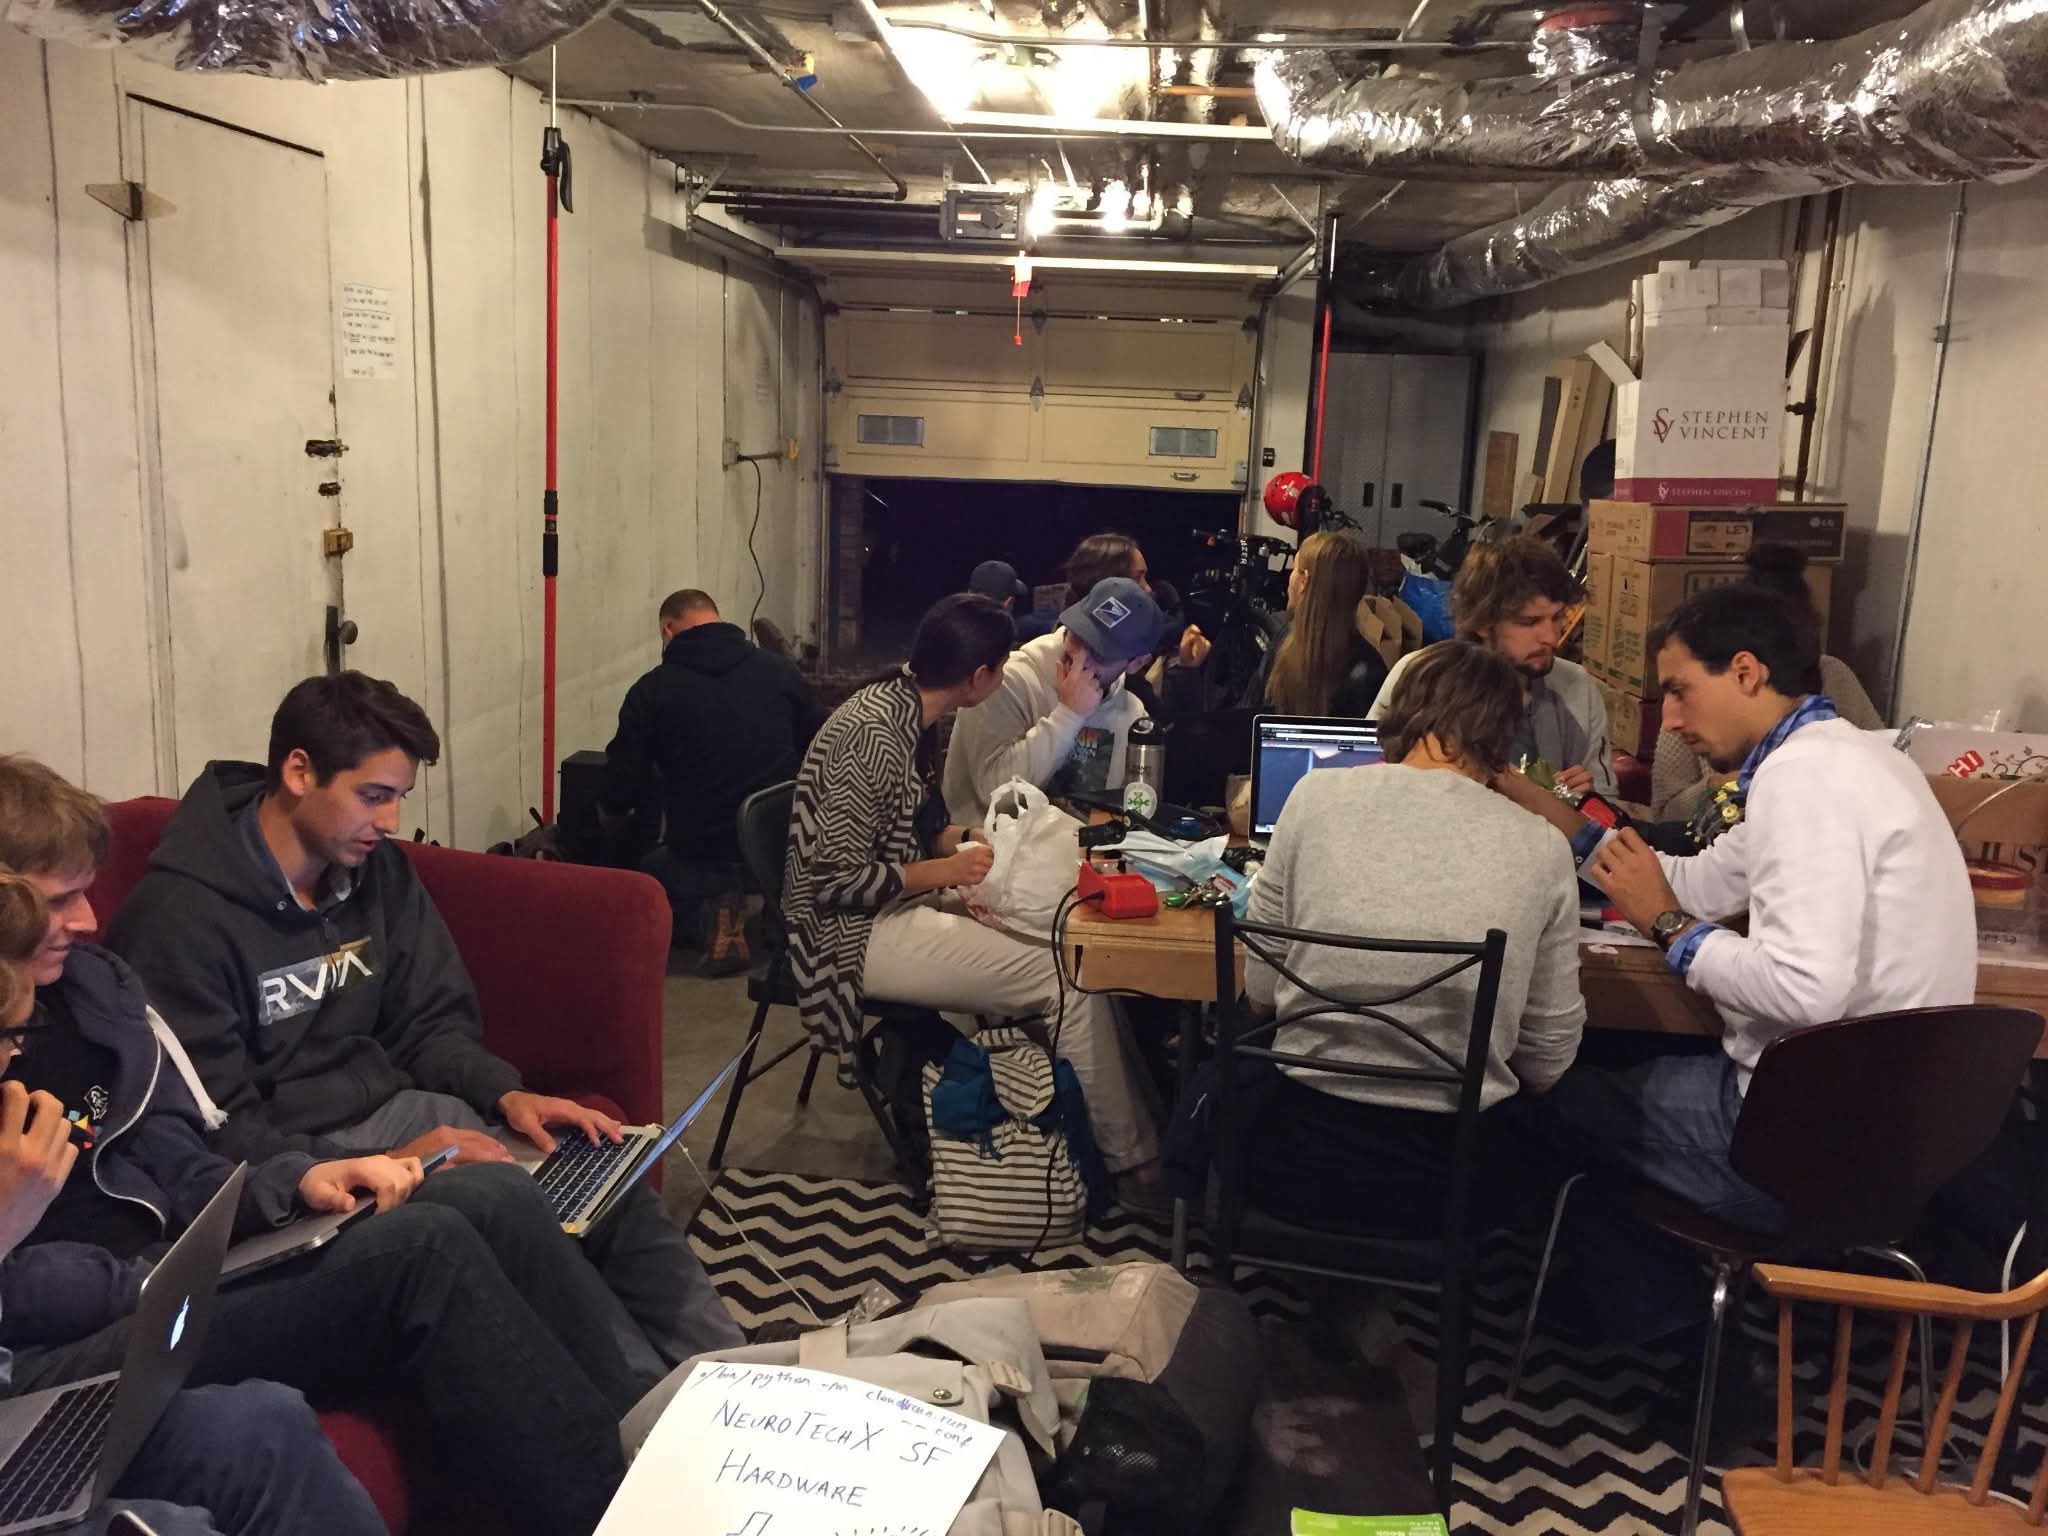
\includegraphics[width=\linewidth,height=44mm,keepaspectratio]{assets/chapters/san-francisco-original-hacknight.jpg}\par\smallskip
      {\scriptsize Start by working on something together\newline Original SF Hacknights --- Morgan's photo\par}
  \end{columns}
  
  \note{[27:15--28:15] Founders can bring useful questions, reproducible examples, teaching and mentoring. Relationships form through doing work together. Community support is reciprocal; this is not a promise of investment, clinical access, regulatory services or cofounder matching.}
\end{frame}

\section{Acknowledgements}

% Selected from slides.tex
\begin{frame}{Acknowledgements}
  \begin{columns}[T,onlytextwidth]
    \column{.47\textwidth}
      \textbf{Board Members}\par\smallskip
      \begin{minipage}[t]{.48\linewidth}
        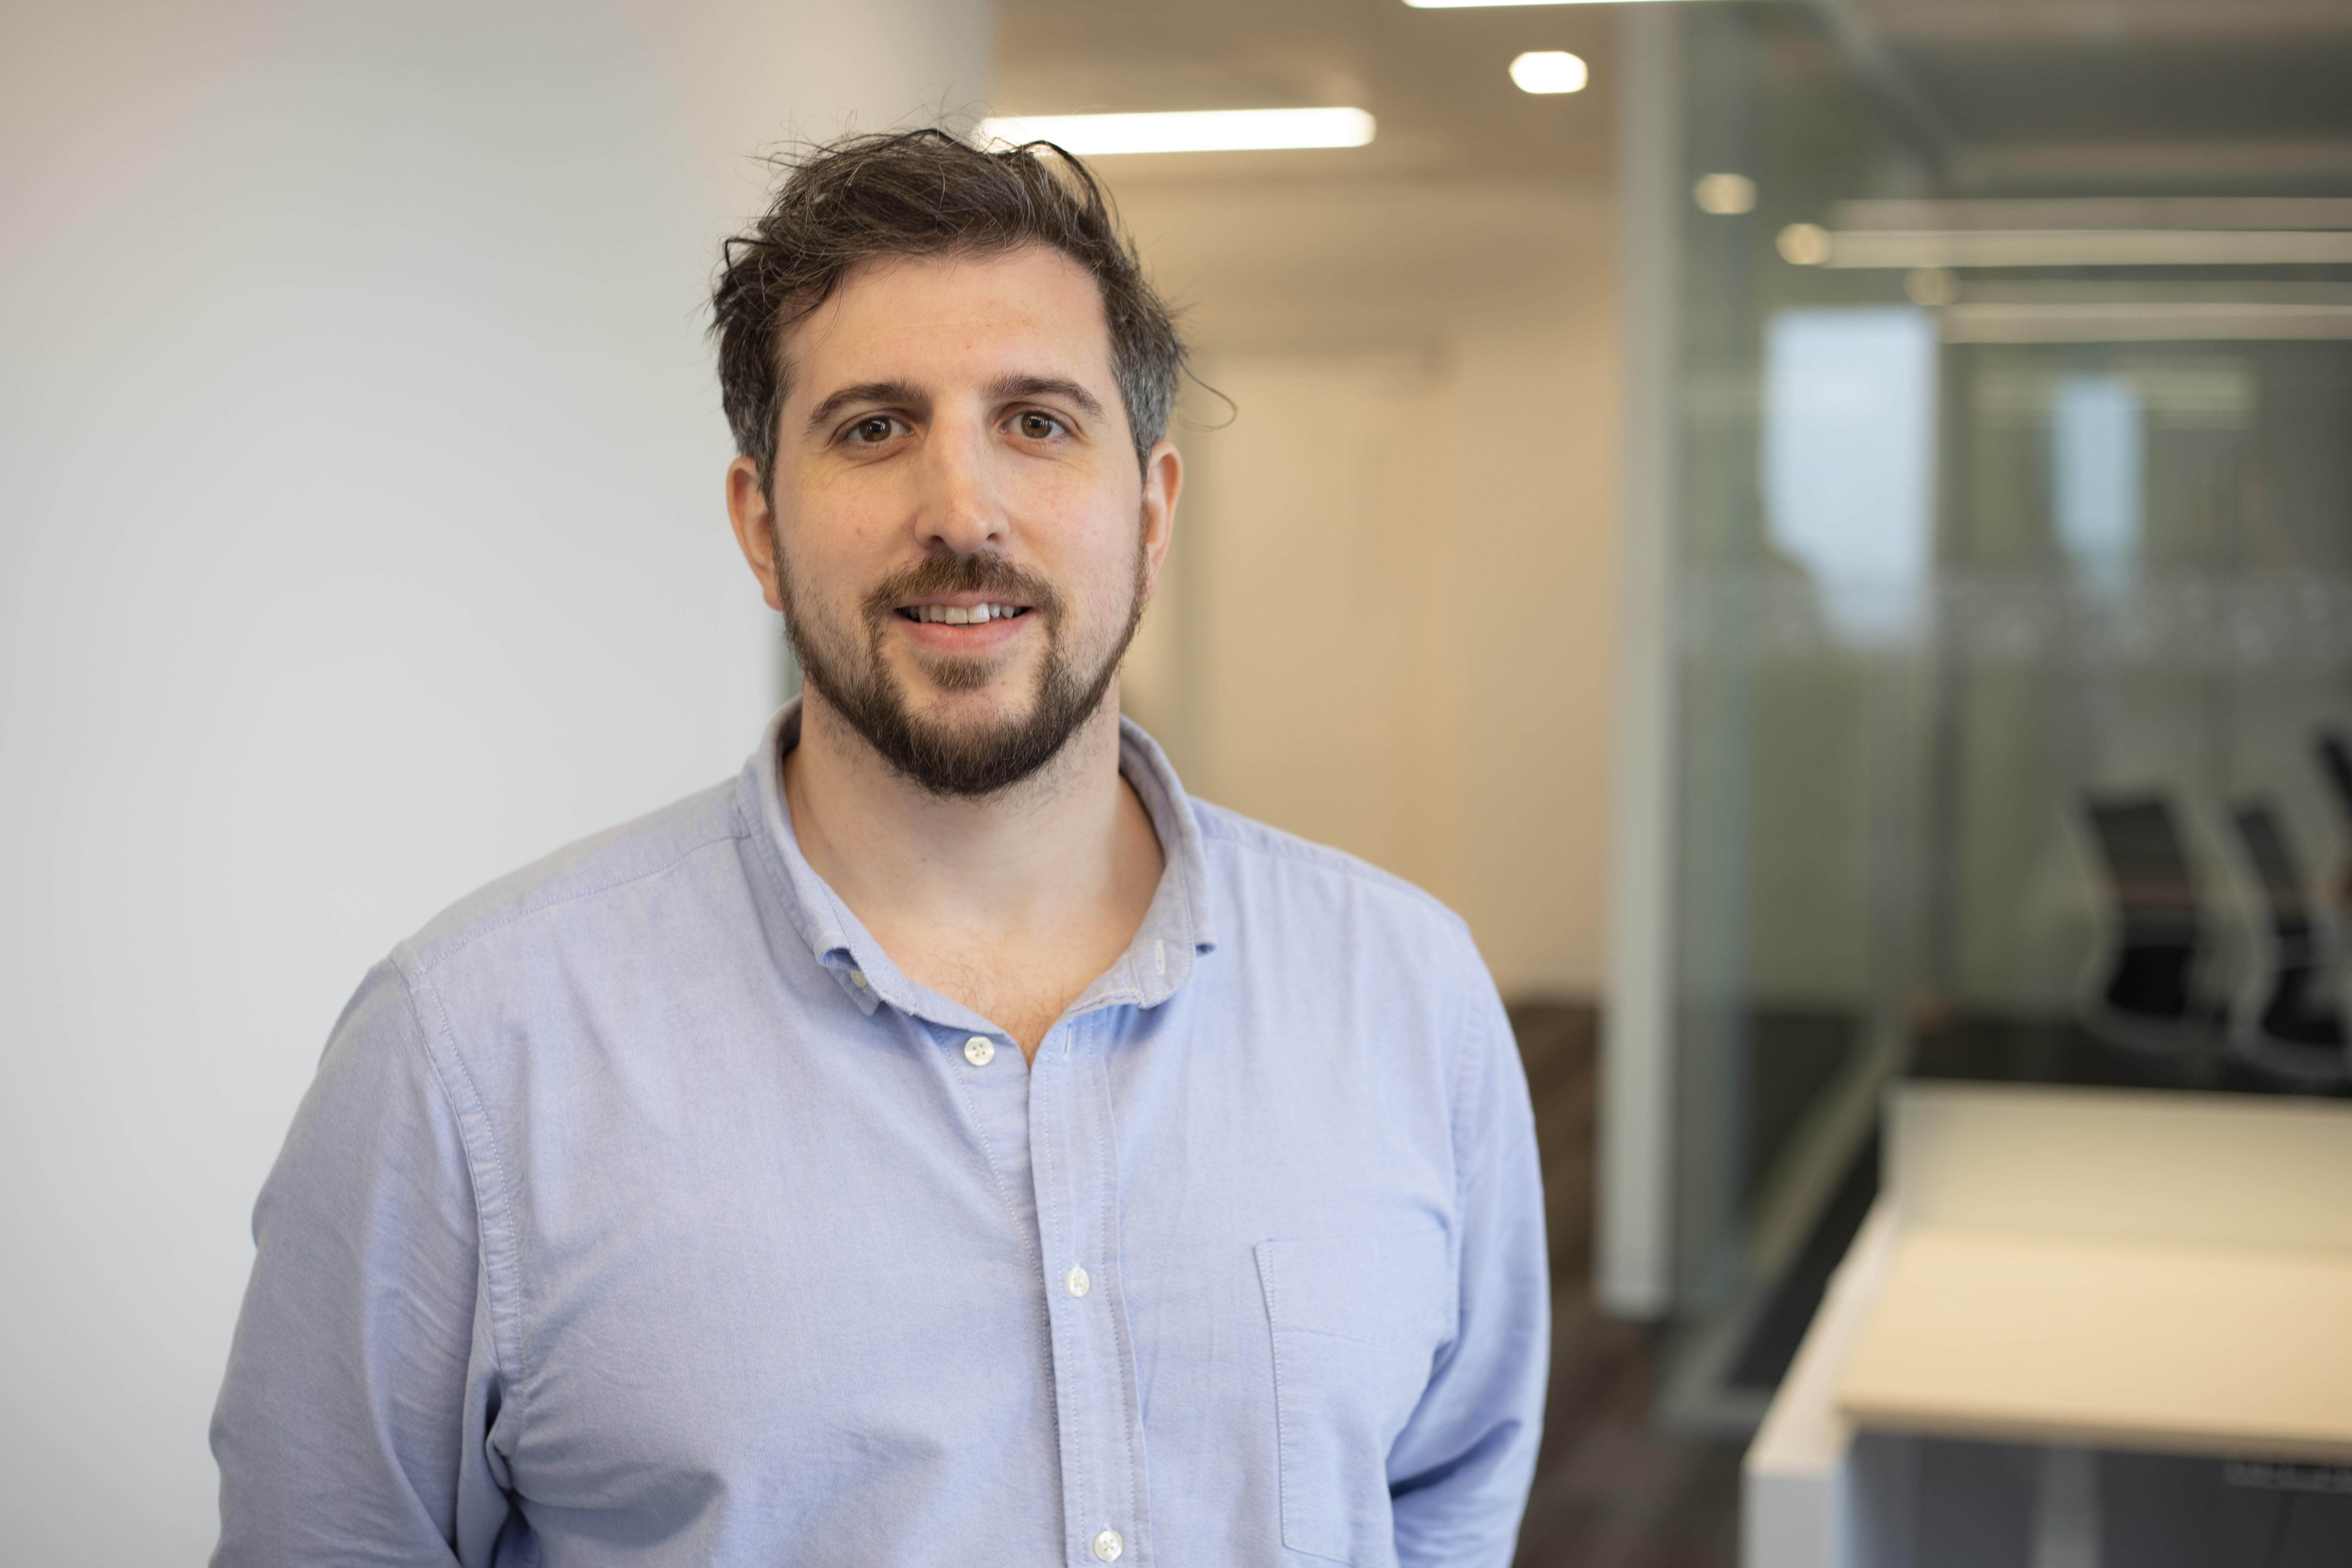
\includegraphics[width=\linewidth,height=21mm,keepaspectratio]{assets/people/john-griffiths.jpg}
        \par\smallskip{\small John Griffiths\par}
      \end{minipage}\hfill
      \begin{minipage}[t]{.48\linewidth}
        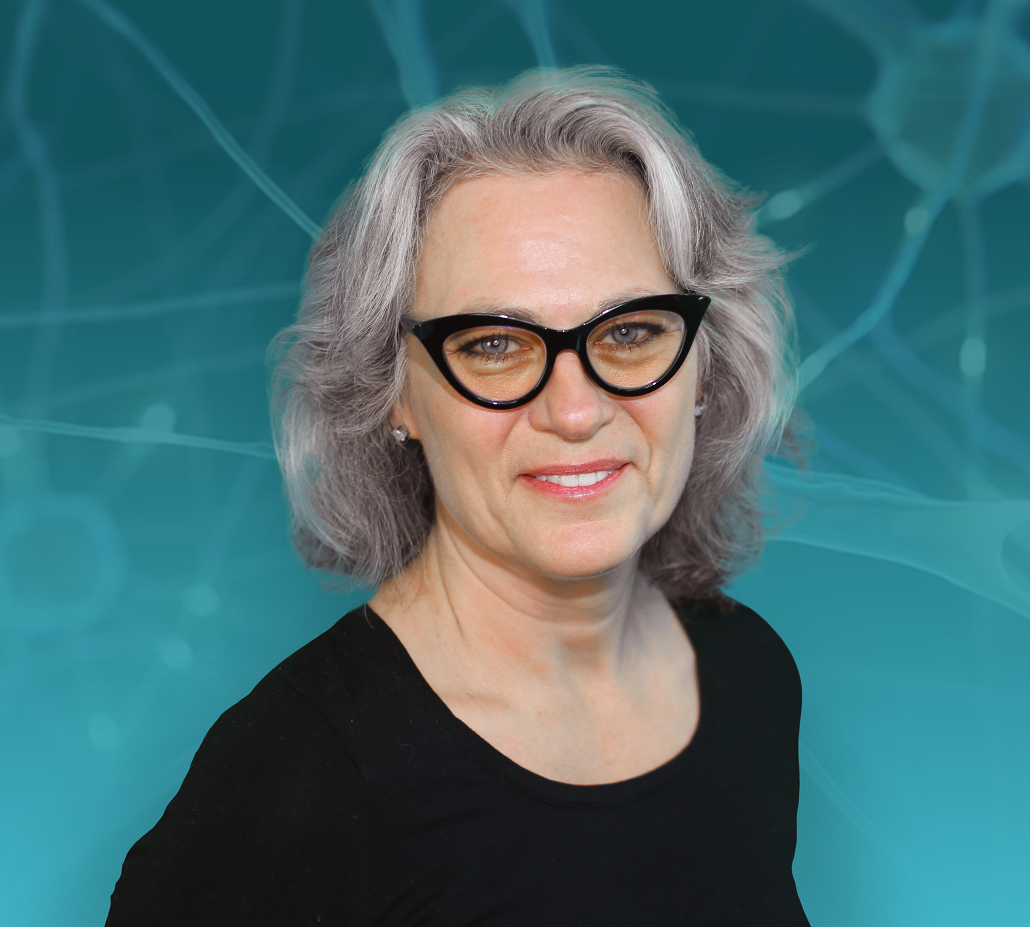
\includegraphics[width=\linewidth,height=21mm,keepaspectratio]{assets/people/susan-boehnke.png}
        \par\smallskip{\small Susan Boehnke\par}
      \end{minipage}
      \par\medskip
      {\small
        \textbf{BCIWiki} --- Landon Burress\par\medskip
        \textbf{MOABB} --- Bruno Aristimunha\par
        Lead developer\par\medskip
        \textbf{NeuroTechX SLC} --- Leonardo Ferrisi\par
      }
    \column{.48\textwidth}
      \small
      \setlength{\medskipamount}{3pt}
      \NTXPoint{Officers}{Han Nyguen and Dhruv Mehrotra}
      \NTXPoint{NTX Content Laboratory}{Sophie Valentine}
      \NTXPoint{CogLab / Learning Planet Institute}{Romain Rouyer and Hans Rajoharison}
      \NTXPoint{NeuroTechX Berlin}{Cris Michelli and Mitch Altman}
      \NTXPoint{Greater Bay Area}{Kimberley Cheung\newline Hong Kong / Shenzhen / Guangzhou}
  \end{columns}
  \medskip
  {\tiny\color{NTXMuted}Portraits: \href{https://www.camh.ca/en/science-and-research/science-and-research-staff-directory/john-griffths}{CAMH}; \href{https://neurotechmicrocreds.com/our-team/susan-boehnke-phd/}{Queen's NeuroTech Microcredential Program}\par}

  \note{[28:15--28:45] Thank the board, officers, content team, chapter organizers and open-source contributors shown here. The full deck contains detailed name and portrait provenance. Keep this brief and finish on the invitation.}
\end{frame}

\section{Join the community}

% Selected from slides.tex
\begin{frame}{What can we build and learn together?}
  \begin{columns}[T,onlytextwidth]
    \column{.48\textwidth}
      \centering
      \textbf{Join NTX}\par\smallskip
      {\setlength{\fboxsep}{3mm}\colorbox{white}{\color{black}\qrcode[height=31mm,level=M,hyperlink=false]{https://bit.ly/ntx-slack}}}\par\smallskip
      {\small\href{https://bit.ly/ntx-slack}{bit.ly/ntx-slack}\par}
      {\scriptsize NeuroTechX Slack community\par}
    \column{.48\textwidth}
      \centering
      \textbf{Slides \& LaTeX repo}\par\smallskip
      {\setlength{\fboxsep}{3mm}\colorbox{white}{\color{black}\qrcode[height=31mm,level=M,hyperlink=false]{https://github.com/m9h/neurotechx-presentations}}}\par\smallskip
      {\scriptsize\href{https://github.com/m9h/neurotechx-presentations}{github.com/m9h/neurotechx-presentations}\par}
      {\scriptsize\color{NTXMuted}Public repository --- slides and LaTeX source\par}
  \end{columns}
  \medskip
  {\small Morgan Hough \quad \href{mailto:mhough@neurotechx.com}{mhough@neurotechx.com}\par}

  \note{[28:45--29:45] Invite people to join NTX Slack and write to Morgan. Ask what existing groups in Japan could build together, who can host a recurring gathering, and which student project could continue after its first demo. The slides repository is public: the QR code opens the source and downloadable PDFs. Planned remarks end at 29:45; allow questions within the remaining event slot.}
\end{frame}
